\documentclass[xcolor={x11names},10pt]{beamer}

\usetheme{metropolis}
\metroset{numbering=fraction}
\metroset{block=fill}

\newcommand{\backupbegin}{
  \newcounter{finalframe}
  \setcounter{finalframe}{\value{framenumber}}
}
\newcommand{\backupend}{
  \setcounter{framenumber}{\value{finalframe}}
}

\usepackage{headings/kmath}
% Tikz
\usetikzlibrary{calc}
\usetikzlibrary{mindmap,trees,shapes,arrows,backgrounds,topaths}
\usetikzlibrary{decorations.pathmorphing, shapes.geometric}

% Text
\usepackage{enumitem}
\usepackage{ulem}
\usepackage{pifont}

% Maths
\usepackage{amsmath}
\usepackage{amsfonts}
\usepackage{amsthm}
\usepackage{amsopn}

% Plots
\usepackage{pgfplots}
\usepgfplotslibrary{groupplots}

% Tables
\usepackage{booktabs}
\usepackage{array}
\newcolumntype{L}{>$l<$}
\arraycolsep=1.4pt
\setlength{\tabcolsep}{3pt}

% Objective values and functions
\newcommand{\pobj}{p}
\newcommand{\robj}{r}
\newcommand{\dobj}{d}

% Variables
\newcommand{\pvletter}{x}
\newcommand{\dvletter}{u}
\newcommand{\bvletter}{z}
\newcommand{\pv}{\mathbf{\pvletter}}
\newcommand{\dv}{\mathbf{\dvletter}}
\newcommand{\bv}{\mathbf{\bvletter}}
\newcommand{\pvi}[1]{\pvletter_{#1}}
\newcommand{\dvi}[1]{\dvletter_{#1}}
\newcommand{\bvi}[1]{\bvletter_{#1}}

% Problem data
\newcommand{\pdim}{n}
\newcommand{\ddim}{m}
\newcommand{\dic}{\mathbf{A}}
\newcommand{\obs}{\mathbf{y}}
\newcommand{\reg}{\lambda}
\newcommand{\lfunc}{f}
\newcommand{\pfunc}{h}
\newcommand{\rfunc}{g}

% Indices
\newcommand{\idxentry}{i}

% BnB
\newcommand{\setidx}{\mathcal{S}}
\newcommand{\setzero}{\setidx_0}
\newcommand{\setone}{\setidx_1}
\newcommand{\setnone}{\setidx_\bullet}
\newcommand{\nodeSymb}{\nu}
\newcommand{\node}[1]{#1^{\nodeSymb}}

% Math operators
\DeclareMathOperator{\dom}{dom}
\DeclareMathOperator{\interior}{int}

% Math misc
\newcommand{\1}{\mathbf{1}}
\newcommand{\0}{\mathbf{0}}
\newcommand{\abs}[1]{|#1|}
\newcommand{\biconj}[1]{#1^{**}}
\newcommand{\conj}[1]{#1^{*}}
\newcommand{\icvx}{\mathbf{I}}
\newcommand{\intervint}[2]{[#1,#2]}
\newcommand{\iter}[2]{#1^{(#2)}}
\newcommand{\norm}[2]{\|#1\|_#2}
\newcommand{\opt}[1]{#1^{\star}}
\newcommand{\separable}[2]{#1_{#2}}
\newcommand{\subdiff}{\partial}
\newcommand{\transp}[1]{#1^{\mathrm{T}}}


\newenvironment<>{blockcolor}[2]{%
  \setbeamercolor{block title}{fg=#1,bg=#1!15}%
  \setbeamercolor{block body}{fg=#1,bg=#1!15}%
  \begin{block}#3{\centering#2}
}{%
  \end{block}
}

\definecolor{TolLightWhite}{HTML}{FAFAFA}
\definecolor{TolLightOrange}{HTML}{ECA244}

\begin{document}

\begin{frame}[plain,noframenumbering]
  \begin{center}
    {\large\textbf{Branch-and-Bound algorithms \\ for $\boldsymbol{\ell}_{\boldsymbol{0}}$-regularized problems}}
  \end{center}
  \begin{center}
    Théo Guyard \\
    {\small{Inria and Insa Rennes}} \\
    {\small{PhD defense - November 27th, 2024}}
  \end{center}
\end{frame}

% \begin{frame}{$\boldsymbol{\ell}_0$-regularized problems}
    \begin{tikzpicture}[remember picture,overlay]
        \begin{scope}[xshift=0.5\textwidth]
            \onslide<1-> {
                \node[align=center,text width=0.45\textwidth] (problem) at (0,2.5) {
                \begin{blockcolor}{mDarkTeal}{Problem}
                    \centering
                    $\min_{\pv \in \kR^{\pdim}} \lfunc(\dic\pv) + \reg\norm{\pv}{0} + \pfunc(\pv)$
                \end{blockcolor}
                };
            }
            %
            %
            %
            \onslide<2-> {
                \node (loss) at (-4,0) {\textbf{1) Loss} $\lfunc(\dic\pv)$};
                \node [text width=0.35\linewidth, align=center,font=\small,anchor=north] at ($(loss)+(0,-0.35)$) {Models the quantity to minimize in the \textcolor{TolLightOrange}{application} at hand};
            }
            %
            %
            %
            \onslide<3-> {
                \node (norm) at (0,0) {\textbf{2) $\ell_0$-norm} $\norm{\pv}{0}$};
                \node [text width=0.325\linewidth, align=center,font=\small,anchor=north] at ($(norm)+(0,-0.35)$) {Counts non-zeros in its input to promote \\ \textcolor{TolLightOrange}{sparse} solutions};
            }
            %
            %
            %
            \onslide<4-> {
                \node (penalty) at (4,0) {\textbf{3) Penalty} $\pfunc(\pv)$};
                \node [text width=0.35\linewidth, align=center,font=\small,anchor=north] at ($(penalty)+(0,-0.35)$) {Linked to the \textcolor{TolLightOrange}{application} or artificially introduced to enable \textcolor{TolLightOrange}{solution methods}};
            }
            %
            %
            %
            \onslide<5-> {
                \node (sol) at (0,-3.5) {Solutions};
                \draw[->,ultra thick] (sol.west) .. controls ($(loss)+(0,-3.5)$) .. ($(loss)+(0,-2)$) node[midway,fill=TolLightWhite,draw,ultra thick,font=\small] {small loss};
                \draw[->,ultra thick] (sol.east) .. controls ($(penalty)+(0,-3.5)$) .. ($(penalty)+(0,-2)$) node[midway,fill=TolLightWhite,draw,ultra thick,font=\small,inner sep=3pt] {small penalty};
                \draw[->,ultra thick] (sol.north) -- ($(norm)+(0,-2)$) node[midway,fill=TolLightWhite,draw,ultra thick,font=\small] {few non-zeros};
            }
            %
            %
            %
            \onslide<6-> {
                \node[font=\small] (tuning) at (3,1) {tradeoff parameter $\reg > 0$};
                \draw[ultra thick,->] (tuning.west) .. controls (0.4,1.25) .. (0.4,1.75);
            }
        \end{scope}
    \end{tikzpicture}
\end{frame}

\begin{frame}{One problem to rule them all}
    \begin{tikzpicture}[remember picture,overlay]
        \begin{scope}[xshift=0.5\textwidth]
            \onslide<1-> {
                \begin{scope}[yshift=50,scale=0.725]
                    \path[
                        mindmap,
                        concept color=mDarkTeal, 
                        level 1 concept/.append style={
                            minimum size    = 1.5cm,
                            text width      = 1.5cm,
                            level distance  = 4.25cm,
                            sibling angle   = 60,
                            font            = \small,
                        },
                        level 2 concept/.append style={
                            minimum size    = 1.1cm,
                            text width      = 1.1cm,
                            level distance  = 2.75cm,
                            sibling angle   = 45,
                            font            = \scriptsize,
                        }
                    ]
                    node[concept,text=white,minimum size=1.6cm,text width=2.25cm] {\normalsize\textbf{Applications}}
                    [clockwise from=0]
                    child[concept color=TolLightRed!40] {
                        node[concept] {\textbf{signal processing}}
                        [clockwise from=45]
                        child { node[concept] {signal denoising} }
                        child { node[concept] {sparse decoding} }
                        child { node[concept] {phase retrieval} }
                        child { node[concept] {DOA design} }
                    }  
                    child[concept color=TolLightBrown!40] {
                        node[concept] {\small\textbf{operation research}}
                        [clockwise from=337.5]
                        child { node[concept] {portfolio optim.} }
                        child { node[concept] {network design} }
                        child { node[concept] {facility location} }
                    }
                    child[concept color=TolLightGreen!40] {
                        node[concept] {\small\textbf{algebra}}
                        [clockwise from=-67.5]
                        child { node[concept] {sparse factor.} }
                        child { node[concept] {low-rank factor.} }
                        child { node[concept] {feasible system} }
                    }
                    child[concept color=TolDarkBlue!40] {
                        node[concept] {\small\textbf{statistics \& ML}} 
                        [clockwise from=-90]
                        child { node[concept] {sparse PCA} }
                        child { node[concept] {sparse SVM} }
                        child { node[concept] {dictionary learning} }
                        child { node[concept] {feature selection} }
                    };
                \end{scope}
                %
                \node at (0,-4) {A. Tillmann \textit{et. al} (2024)};
            }
            %
            %
            %
            \onslide<2> {
                \node[draw,ultra thick,fill=TolLightWhite,font=\small,text width=0.3\linewidth,align=center] at (-4,1.25) {Sparsity linked to \\ model explainability};
            }
            %
            %
            %
            \onslide<3> {
                \node[draw,ultra thick,fill=TolLightWhite,font=\small,text width=0.3\linewidth,align=center] at (-2,-2.25) {Sparsity linked to \\ matrix rank};
            }
            %
            %
            %
            \onslide<4> {
                \node[draw,ultra thick,fill=TolLightWhite,font=\small,text width=0.3\linewidth,align=center] at (2,-2.25) {Sparsity linked to \\ unit cost count};
            }
            %
            %
            %
            \onslide<5> {
                \node[draw,ultra thick,fill=TolLightWhite,font=\small,text width=0.3\linewidth,align=center] at (4,1.25) {Sparsity linked to \\ signal spikes};
            }
        \end{scope}
    \end{tikzpicture}
\end{frame}
  
\begin{frame}{Solution methods}
    \begin{tikzpicture}[remember picture,overlay]
        \begin{scope}[xshift=0.5\textwidth]
            \onslide<1-> {
                \node[text width=0.45\linewidth, align=center] (problem) at (0,3) {
                    \begin{blockcolor}{mDarkTeal}{Problem}
                        \centering
                        $\min_{\pv \in \kR^{\pdim}} \lfunc(\dic\pv) + \reg\norm{\pv}{0} + \pfunc(\pv)$
                    \end{blockcolor}
                };
                %
                \node[draw,ultra thick] (question) at (0,1.25) {How to design \textcolor{TolLightOrange}{generic} and \textcolor{TolLightOrange}{efficient} solution methods ?};
                \node at ($(question)+(0,0.5)$) {\textbf{Question}};
            }
            %
            %
            %
            \onslide<2-> {
                \node (origin) at (-2,-2.75) {};
                \node at ($(origin)+(0,2.2)$) {\textbf{$\boldsymbol{\ell}_{\0}$-norm in 1d}};
                \node at ($(origin)+(-0.2,-0.2)$) {$0$};
                \node at ($(origin)+(-0.2,1.2)$) {$1$};
                \draw[ultra thick,->] ($(origin)+(-2,0)$) -- ($(origin)+(2,0)$) node[right] {$\pvi{}$};
                \draw[ultra thick,->] ($(origin)+(0,-0.2)$) -- ($(origin)+(0,2)$);
                \draw[-,ultra thick,TolLightOrange] ($(origin)+(-0.1,1)$) -- ($(origin)+(-1.8,1)$);
                \draw[-,ultra thick,TolLightOrange] ($(origin)+(0.1,1)$) -- ($(origin)+(1.8,1)$) node[above] {$\norm{\pvi{}}{0}$};
                \draw[TolLightOrange,ultra thick] ($(origin)+(0,1)$) circle (0.1);
                \fill[TolLightOrange] (origin) circle (0.1);
            }
            %
            %
            %
            \onslide<3-> {
                \node[text width=0.3\linewidth,align=left] (prop) at (3,-0.75) {\textbf{Properties} \\ $\ \ \bullet$ non-convex \\ $\ \ \bullet$ non-smooth \\ $\ \ \bullet$ non-continuous \\ $\ \ \bullet$ ...};
            }
            %
            %
            %
            \onslide<4-> {
                \node[text width=0.4\linewidth,align=center] (hard) at (3,-3.25) {\textbf{Can be tackled using \\ generic MIP solvers} \\ D. Bertsimas \textit{et. al} (2016)};
                \draw[ultra thick,->] ($(prop.south)+(0,-0.1)$) -- ($(hard.north)+(0,0.1)$);
            }
        \end{scope}
    \end{tikzpicture}
\end{frame}

\begin{frame}{Numerics}
    \begin{tikzpicture}[remember picture,overlay]
        \begin{scope}[xshift=0.5\textwidth]
            \onslide<1-> {
                \node[text width=0.45\linewidth, align=center] (problem) at (0,3) {
                    \begin{blockcolor}{mDarkTeal}{Problem}
                        \centering
                        $\min_{\pv \in \kR^{\pdim}} \lfunc(\dic\pv) + \reg\norm{\pv}{0} + \pfunc(\pv)$
                    \end{blockcolor}
                };
                %
                \node[font=\small] at ($(problem)+(0,-1)$) {$\dic \in \kR^{100\times300}$ / $\lfunc:$ Quadratic / $\pfunc:$ Bound constraint};
            }
            %
            %
            %
            \onslide<3-> {
            \node[text width=0.6\linewidth,align=left,font=\small] at (2.75,-1) {\textbf{MIP solvers} \\ \ref{plot:mip-Scip} Scip \\ \ref{plot:mip-Cplex} Cplex \\ \ref{plot:mip-Mosek} Mosek};
            }
            %
            %
            %
            \onslide<4-> {
                \node[text width=0.3\linewidth,align=center] (obs) at ($(problem)+(3.75,-2.75)$) {\textbf{Can we do better ?}};
            }
            %
            %
            %
            \onslide<5-> {
            \node[text width=0.45\linewidth,align=center] (sol) at ($(obs.south)+(0,-1.5)$) {\textbf{BnB solvers} \\ Specialized for the problem at hand};
            \draw[ultra thick,->] ($(obs.south)+(0,-0.1)$) -- ($(sol.north)+(0,0.1)$);
            }
        \end{scope}
        \begin{scope}[xshift=0.075\linewidth,yshift=-65]
            %
            \pgfplotscreateplotcyclelist{cycle_perfprofiles_mip}{
                TolDarkBlue, very thick, smooth\\    
                TolLightBlue, very thick, smooth\\
                TolLightGreen, very thick, smooth\\
            }
            %
            \onslide<2-> {
                \draw[very thick,dotted] (3.6,0) -- (3.6,2.5) node[above,font=\scriptsize] {1 hour};
            }
            %
            %
            %
            \onslide<2> {
                \begin{axis}[
                    width   = 0.5\textwidth,
                    height  = 0.4\textwidth,,
                    legend style={
                        at={(1,0.5)},
                        anchor=west,
                        legend columns=1, 
                        /tikz/every even column/.style = {column sep=5pt},
                        draw=none
                    },
                    cycle list name=cycle_perfprofiles_mip,
                    mbaseplot,
                    axis line style = ultra thick,
                    major tick style = {ultra thick,color=mDarkTeal},
                    xmajorgrids=true,
                    ymajorgrids=true,
                    major grid style={dotted},
                    axis x line=bottom,
                    axis y line=left,
                    xmode=log,
                    minor tick style={draw=none},
                    xlabel=\textbf{\small{Time (seconds)}},
                    ymax=110,
                    ymin=0,
                    xmin=0.01,
                    xmax=7000,
                    ylabel=\textbf{\small{Instances solved}},
                    ytick={0,25,50,75,100},
                ]
                \end{axis}
            }
            %
            %
            %
            \onslide<3-> {
                \begin{axis}[
                    width   = 0.5\textwidth,
                    height  = 0.4\textwidth,,
                    legend style={
                        at={(1,0.5)},
                        anchor=west,
                        legend columns=1, 
                        /tikz/every even column/.style = {column sep=5pt},
                        draw=none
                    },
                    cycle list name=cycle_perfprofiles_mip,
                    mbaseplot,
                    axis line style = ultra thick,
                    major tick style = {ultra thick,color=mDarkTeal},
                    xmajorgrids=true,
                    ymajorgrids=true,
                    major grid style={dotted},
                    axis x line=bottom,
                    axis y line=left,
                    xmode=log,
                    minor tick style={draw=none},
                    xlabel=\textbf{\small{Time (seconds)}},
                    ymax=110,
                    ymin=0,
                    xmin=0.01,
                    xmax=7000,
                    ylabel=\textbf{\small{Instances solved}},
                    ytick={0,25,50,75,100},
                ]
                    \foreach \solver in {Scip,Cplex,Mosek} {
                        \addplot table[
                            x=times,
                            y expr=100*\thisrow{\solver},
                            col sep=comma
                        ] {data/perfprofiles_medium_Leastsquares_Bigm_3600.csv};
                        \label{plot:mip-\solver}
                    }
                \end{axis}
            }
        \end{scope}
    \end{tikzpicture}
\end{frame}
% \section{Branch-and-Bound Algorithms}

\begin{frame}{BnB -- Algorithmic principle}
  \begin{tikzpicture}[remember picture,overlay]
    \begin{scope}[xshift=0.5\textwidth]
      \onslide<1-> {
        \node[text width=\textwidth,align=center] at (0,3.25) {Explore \textcolor{TolLightOrange}{regions} in the feasible space and \textcolor{TolLightOrange}{prune} those \\ that cannot contain any optimal solution.};
      }
      %
      %
      %
      \onslide<2-> {
        \draw[ultra thick, fill=gray!20,rotate=15] (0,0) ellipse (3.5cm and 1.75cm);
        \node[rotate=15] at (-0.5,1.25) {\small{Feasible space}};
      }
      %
      %
      %
      \onslide<3-> {
        \draw[ultra thick, fill=gray!40,rotate=30] (1,-1) ellipse (1cm and 0.75cm);
        \node[rotate=15] at (1.4,0) {\small{Region $\nodeSymb$}};
      }
      %
      %
      %
      \onslide<4-> {
        \draw[ultra thick,<-] (2.3,-0.25) .. controls(3.5,-0.5) .. (4,-1) node[below] {\textbf{Pruning test}};
      }
      %
      %
      %
      \onslide<5-> {
        \node[font=\small] at (4,-1.75) {No solution in region $\nodeSymb$};
        \draw[ultra thick,fill=TolLightRed!50,rotate=30] (1,-1) ellipse (1cm and 0.75cm);
        \node[rotate=15] at (1.4,0) {\small{Region $\nodeSymb$}};
      }
      %
      %
      %
      \onslide<6-> {
        \node at (0,-3.25) {$\begin{array}{lcl}\textbf{Branching} &\textbf{--}& \text{Region management} \\  \textbf{Bounding}  &\textbf{--}& \text{Pruning test evaluation} \end{array}$};
      }
    \end{scope}
  \end{tikzpicture}
\end{frame}

\begin{frame}{BnB -- How to construct regions in the feasible space ?}
  \begin{tikzpicture}[remember picture,overlay]
    \begin{scope}[xshift=0.5\textwidth]
      \onslide<1-> {
        \node[text width=0.45\linewidth, align=center] (problem) at (0,3.25) {
          \begin{blockcolor}{mDarkTeal}{Problem}
              \centering
              $\min_{\pv \in \kR^{\pdim}} \lfunc(\dic\pv) + \reg\norm{\pv}{0} + \pfunc(\pv)$
          \end{blockcolor}
        };
      }
      %
      %
      %
      \onslide<2-> {
        \node[text width=0.4\linewidth,align=center] (obs) at ($(problem)+(-4,-1.5)$) {\textbf{Observation} \\ Solutions expected \\ to be sparse};
      }
      %
      %
      %
      \onslide<3-> {
        \node[text width=0.4\linewidth,align=center] (method) at ($(problem)+(4,-1.5)$) {\textbf{Method} \\ Drive the sparsity of the optimization variable};
      }
      %
      %
      %
      \onslide<4-> {
        \node at (0,0.75) (node0) {};
        \node at ($(node0)+(0,1)$) {\small{$\kR^{\pdim}$}};
        \draw[ultra thick,->] ($(node0)+(0,0.8)$) -- ($(node0)+(0,0.5)$);
        \draw[
            ultra thick,
            top color = white,
            bottom color = gray!60,
        ] (node0) circle (10pt) node {$\nodeSymb_0$};
      }
      %
      %
      %
      \onslide<5-> {
        \node at ($(node0)+(-3,-0.75)$) (node1) {};
        \draw[
            ultra thick,
            top color = white,
            bottom color = gray!60,
        ] (node1) circle (10pt) node {$\nodeSymb_1$};
        \draw[ultra thick,->] ($(node0.south west)+(-0.2,0)$) -- ($(node1.east)+(0.2,0.2)$) node[midway,fill=TolLightWhite,draw,font=\scriptsize,inner sep=2] {$\pvi{1} = 0$};
        %
        \node at ($(node0)+(3,-0.75)$) (node2) {};
        \draw[
            ultra thick,
            top color = white,
            bottom color = gray!60,
        ] (node2) circle (10pt) node {$\nodeSymb_2$};
        \draw[ultra thick,->] ($(node0.south east)+(0.2,0)$) -- ($(node2.west)+(-0.2,0.2)$) node[midway,fill=TolLightWhite,draw,font=\scriptsize,inner sep=1.75] {$\pvi{1} \neq 0$};
        %
        \draw[
          ultra thick,
          top color = white,
          bottom color = gray!60,
        ] (node2) circle (10pt) node {$\nodeSymb_2$};
      }
      %
      %
      %
      \onslide<6> {
        \node[font=\scriptsize,text width=0.2\linewidth,align=center,anchor=north] at ($(node1)+(0,-0.5)$) {\textbf{Pruning test} \\ Solutions in $\nodeSymb_1$ ?};
        \node[font=\scriptsize,text width=0.2\linewidth,align=center,anchor=north] at ($(node2)+(0,-0.5)$) {\textbf{Pruning test} \\ Solutions in $\nodeSymb_2$ ?};
      }
      %
      %
      %
      \onslide<7> {
        \node[font=\scriptsize,text width=0.2\linewidth,align=center,anchor=north] at ($(node1)+(0,-0.5)$) {\textbf{Pruning test} \\ Solutions in $\nodeSymb_1$ ?};
        \node[font=\scriptsize,text width=0.2\linewidth,align=center,anchor=north] at ($(node2)+(0,-0.5)$) {\textbf{Pruning test} \\ Solutions in $\nodeSymb_2$ ? \\ \textcolor{TolLightRed}{No}};
      }
      %
      %
      %
      \onslide<7-> {
        \draw[
            ultra thick,
            top color = white,
            bottom color = TolLightRed,
        ] (node2) circle (10pt) node {$\nodeSymb_{2}$};
      }
      %
      %
      %
      \onslide<8> {
        \node[font=\scriptsize,text width=0.2\linewidth,align=center,anchor=north] at ($(node1)+(0,-0.5)$) {\textbf{Pruning test} \\ Solutions in $\nodeSymb_1$ ? \\ \textcolor{gray}{Maybe}};
        \node[font=\scriptsize,text width=0.2\linewidth,align=center,anchor=north] at ($(node2)+(0,-0.5)$) {\textbf{Pruning test} \\ Solutions in $\nodeSymb_2$ ? \\ \textcolor{TolLightRed}{No}};
      }
      %
      %
      %
      \onslide<9-> {
        \node at ($(node1)+(-1.5,-1.25)$) (node3) {};
        \draw[
            ultra thick,
            top color = white,
            bottom color = gray!60,
        ] (node3) circle (10pt) node {$\nodeSymb_3$};
        \draw[ultra thick,->] ($(node1.south west)+(-0.2,0)$) -- ($(node3.north)+(0.2,0.2)$) node[midway,fill=TolLightWhite,draw,font=\scriptsize,inner sep=2] {$\pvi{2} = 0$};
        %
        \node at ($(node1)+(1.5,-1.25)$) (node4) {};
        \draw[
            ultra thick,
            top color = white,
            bottom color = gray!60,
        ] (node4) circle (10pt) node {$\nodeSymb_4$};
        \draw[ultra thick,->] ($(node1.south east)+(0.2,0)$) -- ($(node4.north)+(-0.2,0.2)$) node[midway,fill=TolLightWhite,draw,font=\scriptsize,inner sep=1.75] {$\pvi{2} \neq 0$};
      }
      %
      %
      %
      \onslide<10> {
        \node[font=\scriptsize,text width=0.2\linewidth,align=center,anchor=north] at ($(node4)+(0,-0.5)$) {\textbf{Pruning test} \\ Solutions in $\nodeSymb_4$ ?};
        \node[font=\scriptsize,text width=0.2\linewidth,align=center,anchor=north] at ($(node3)+(0,-0.5)$) {\textbf{Pruning test} \\ Solutions in $\nodeSymb_3$ ?};
      }
      %
      %
      %
      \onslide<11> {
        \node[font=\scriptsize,text width=0.2\linewidth,align=center,anchor=north] at ($(node4)+(0,-0.5)$) {\textbf{Pruning test} \\ Solutions in $\nodeSymb_4$ ? \\ \textcolor{gray}{Maybe}};
        \node[font=\scriptsize,text width=0.2\linewidth,align=center,anchor=north] at ($(node3)+(0,-0.5)$) {\textbf{Pruning test} \\ Solutions in $\nodeSymb_3$ ? \\ \textcolor{TolLightRed}{No}};
      }
      %
      %
      %
      \onslide<11-> {
        \draw[
            ultra thick,
            top color = white,
            bottom color = TolLightRed,
        ] (node3) circle (10pt) node {$\nodeSymb_{3}$};
      }
      %
      %
      %
      \onslide<12-> {
        \node at ($(node4)+(-1.25,-1.35)$) (node5) {};
        \draw[
            ultra thick,
            top color = white,
            bottom color = gray!60,
        ] (node5) circle (10pt) node {$\nodeSymb_{5}$};
        \draw[ultra thick,->] ($(node4.south west)+(-0.125,-0.125)$) -- ($(node5.north)+(0.2,0.2)$) node[midway,fill=TolLightWhite,draw,font=\scriptsize,inner sep=2] {$\pvi{3} = 0$};
        %
        \node at ($(node4)+(1.25,-1.35)$) (node6) {};
        \draw[
            ultra thick,
            top color = white,
            bottom color = gray!60,
        ] (node6) circle (10pt) node {$\nodeSymb_{6}$};
        \draw[ultra thick,->] ($(node4.south east)+(0.125,-0.125)$) -- ($(node6.north)+(-0.2,0.2)$) node[midway,fill=TolLightWhite,draw,font=\scriptsize,inner sep=1.75] {$\pvi{3} \neq 0$};
      }
      %
      %
      %
      \onslide<13> {
        \node[font=\scriptsize,text width=0.2\linewidth,align=center,anchor=north] at ($(node6)+(0,-0.5)$) {\textbf{Pruning test} \\ Solutions in $\nodeSymb_6$ ?};
        \node[font=\scriptsize,text width=0.2\linewidth,align=center,anchor=north] at ($(node5)+(0,-0.5)$) {\textbf{Pruning test} \\ Solutions in $\nodeSymb_5$ ?};
      }
      %
      %
      %
      \onslide<14> {
        \node[font=\scriptsize,text width=0.2\linewidth,align=center,anchor=north] at ($(node6)+(0,-0.5)$) {\textbf{Pruning test} \\ Solutions in $\nodeSymb_6$ ? \\ \textcolor{TolLightRed}{No}};
        \node[font=\scriptsize,text width=0.2\linewidth,align=center,anchor=north] at ($(node5)+(0,-0.5)$) {\textbf{Pruning test} \\ Solutions in $\nodeSymb_5$ ? \\ \textcolor{gray}{Maybe}};
      }
      %
      %
      %
      \onslide<14-> {
        \draw[
            ultra thick,
            top color = white,
            bottom color = TolLightRed,
        ] (node6) circle (10pt) node {$\nodeSymb_{6}$};
      }
      %
      %
      %
      \onslide<16-> {
        \node[font=\scriptsize,text width=0.1\linewidth,align=center,anchor=north] at ($(node5)+(0,-0.5)$) {\textbf{Recover \\ solution}};
      }
      %
      %
      %
      \onslide<17-> {
        \node[text width=0.5\linewidth,align=center] at (3,-2.25) {\textbf{Solve time} \\ nodes processed \\ $\times$ \\ pruning test time};
      }
    \end{scope}
  \end{tikzpicture}
\end{frame}

\begin{frame}{BnB -- How to evaluate a pruning test ?}
  \begin{tikzpicture}[remember picture,overlay]
    \begin{scope}[xshift=0.5\textwidth]
      \onslide<1-> {
        \node at (0,3.25) (nodek) {};
        \draw[
            ultra thick,
            top color = white,
            bottom color = gray!60,
        ] (nodek) circle (10pt) node {$\nodeSymb$};
        \draw[ultra thick,->] ($(nodek.north east)+(0.6,0.4)$) -- ($(nodek.east)+(0.2,0.2)$);
        \node[font=\small,text width=\linewidth,align=center] at ($(nodek)+(0,-1)$) {\textbf{Pruning test} \\ Does region $\nodeSymb$ contain solutions ?};
      }
      %
      %
      %
      \onslide<2-> {
        \node[text width=0.55\linewidth, align=center] (problem) at ($(nodek)+(-2.5,-2.25)$) {
            \begin{blockcolor}{mDarkTeal}{Problem}
                \centering
                $\opt{\pobj} = \min_{\pv \in \kR^{\pdim}} \lfunc(\dic\pv) + \reg\norm{\pv}{0} + \pfunc(\pv)$
            \end{blockcolor}
        };
      }
      %
      %
      %
      \onslide<3-> {
        \node[text width=0.55\linewidth, align=center] (region-problem) at ($(problem)+(0,-2.25)$) {
            \begin{blockcolor}{mDarkTeal}{Restriction to region $\nodeSymb$}
                \centering
                $\node{\pobj} = \min_{\textcolor{TolLightOrange}{\pv \in \nodeSymb} \ } \lfunc(\dic\pv) + \reg\norm{\pv}{0} + \pfunc(\pv)$
            \end{blockcolor}
        };
        \draw[ultra thick,->] ($(problem)+(0,-0.75)$) -- ($(region-problem)+(0,0.5)$) node[midway,fill=TolLightWhite,draw,ultra thick,font=\small] {restrict to $\nodeSymb$};
      }
      %
      %
      %
      \onslide<4> {
        \node[text width=0.25\linewidth,align=center] (pruning) at ($(region-problem)+(0,-2.25)$) {
          \begin{blockcolor}{mDarkTeal}{Pruning test}
            \centering
            $\node{\pobj} > \opt{\pobj}$
          \end{blockcolor}
        };
        \draw[ultra thick,->] ($(region-problem)+(0,-0.75)$) -- ($(pruning)+(0,0.5)$) node[midway,fill=TolLightWhite,draw,ultra thick,font=\small] {compare};
      }
      %
      %
      %
      \onslide<5-> {
        \node[text width=0.25\linewidth,align=center] (pruning) at ($(region-problem)+(0,-2.25)$) {
          \begin{blockcolor}{mDarkTeal}{Pruning test}
            \centering
            $\node{\pobj}_{\textcolor{TolLightOrange}{\text{lb}}} > \opt{\pobj}_{\textcolor{TolLightOrange}{\text{ub}}}$
          \end{blockcolor}
        };
        \draw[ultra thick,->] ($(region-problem)+(0,-0.75)$) -- ($(pruning)+(0,0.5)$) node[midway,fill=TolLightWhite,draw,ultra thick,font=\small] {compare};
      }
      %
      %
      %
      \onslide<6-> {
        \node (easy) at ($(problem)+(6,0)$) {\textbf{Easy task}};
        \node[draw,ultra thick,text width=0.44\linewidth,align=center] (easy-text) at ($(easy.south)+(0,-0.25)$) {Compute an upper bound on $\opt{\pobj}$};
      }
      %
      %
      %
      \onslide<7-> {
        \node[font=\small,text width=0.375\linewidth,align=center,anchor=north] (easy-text2) at ($(easy-text.south)+(0,-0.05)$) {Construct and evaluate a feasible vector in each region explored to refine $\opt{\pobj}_{\text{ub}}$};
      }
      %
      %
      %
      \onslide<8-> {
        \node (easy) at ($(problem)+(6,-3.25)$) {\textbf{Main challenge}};
        \node[draw,ultra thick,text width=0.44\linewidth,align=center] (easy-text) at ($(easy.south)+(0,-0.25)$) {Compute a lower bound on $\node{\pobj}$};
      }
    \end{scope}
  \end{tikzpicture}
\end{frame}

\begin{frame}{BnB -- Standard lower bounding strategy}
  \begin{tikzpicture}[remember picture,overlay]
    \begin{scope}[xshift=0.5\linewidth]
      \onslide<1-> {
        \node[text width=0.525\linewidth, align=center] (restrict) at (0,3) {
          \begin{blockcolor}{mDarkTeal}{Restriction to region $\nodeSymb$}
              \centering
              $\node{\pobj} = \min_{\pv \in \nodeSymb} \lfunc(\dic\pv) + \reg\norm{\pv}{0} + \pfunc(\pv)$
          \end{blockcolor}
        };
      }
      %
      %
      %
      \onslide<2-> {
        \node[text width=0.675\linewidth,align=left] at (0,1.25) {\textbf{Requirement 1 --} Tight lower bound on $\node{\pobj}$};
      }
      %
      \onslide<2-> {
        \node[text width=0.675\linewidth,align=left] at (0,0.75) {\textbf{Requirement 2 --} Tractable lower bound on $\node{\pobj}$};
      }
      %
      %
      %
      \onslide<3-> {
        \node (std) at (0,-0.5) {\textbf{Standard strategy}};
        \node (std-text) at ($(std.south)+(0,-0.1)$) {Construct and solve a \textcolor{TolLightOrange}{relaxation}};
        \draw[ultra thick,->] ($(std)+(0,0.75)$) -- ($(std)+(0,0.4)$);
      }
      %
      %
      %
      \onslide<4-> {
        \draw[very thick] ($(restrict)+(0.6,-0.7)$) -- ($(restrict)+(0.6,-0.75)$) -- ($(restrict)+(2.7,-0.75)$) -- ($(restrict)+(2.7,-0.7)$);
        \node at ($(restrict)+(1.65,-1)$) {$\rfunc(\pv)$};
      }
      %
      %
      %
      \onslide<5-> {
        \node[text width=0.5\linewidth, align=center] (relax) at (0,-1.75) {
          \begin{blockcolor}{mDarkTeal}{Relaxation for region $\nodeSymb$}
              \centering
              $\node{\pobj}_{\text{lb}} = \min_{\pv \in \nodeSymb} \lfunc(\dic\pv) + \textcolor{TolLightOrange}{\rfunc_{\text{lb}}}(\pv)$
          \end{blockcolor}
        };
      }
      %
      %
      %
      \onslide<6-> {
        \node[font=\small,text width=0.2\linewidth,align=left,anchor=west] at ($(relax)+(2.75,-0.1)$) {$\rfunc_{\text{lb}} \leq \rfunc$ \\ $\rfunc_{\text{lb}}$ convex};
      }
      %
      %
      %
      \onslide<7-> {
        \node[TolLightOrange] (lb) at (0,-3) {\textbf{Lower bound}};
        \node[draw,ultra thick,TolLightOrange] (lb-text) at ($(lb.south)+(0,-0.25)$) {$\node{\pobj}_{\text{lb}} \leq \node{\pobj}$};
      }
    \end{scope}
  \end{tikzpicture}
\end{frame}

\begin{frame}{BnB -- Enhanced performance}
  \begin{tikzpicture}[remember picture,overlay]
    \begin{scope}[xshift=0.5\textwidth]
      \onslide<1-> {
        \node[text width=0.45\linewidth, align=center] (problem) at (0,2.75) {
          \begin{blockcolor}{mDarkTeal}{Problem}
              \centering
              $\min_{\pv \in \kR^{\pdim}} \lfunc(\dic\pv) + \reg\norm{\pv}{0} + \pfunc(\pv)$
          \end{blockcolor}
        };
      }
      %
      %
      %
      \onslide<1-2> {
        \node[font=\small] at ($(problem)+(0,-1)$) {$\dic \in \kR^{100\times300}$ / $\lfunc:$ Quadratic / $\pfunc:$ Bound constraint};
        %
        \node[text width=0.6\linewidth,align=left,font=\small] at (2.75,-0.5) {\textbf{MIP solvers} \\ \ref{plot:bnb-Scip} Scip \\ \ref{plot:bnb-Cplex} Cplex \\ \ref{plot:bnb-Mosek} Mosek};
      }
      %
      %
      %
      \onslide<2> {
        \node[text width=0.6\linewidth,align=left,font=\small] at (2.75,-2.1) {\textbf{BnB solvers} \\ \ref{plot:bnb-L0Bnb} L0Bnb -- H. Hazimeh \textit{et al.} (2021) \\ \ref{plot:bnb-SBnb} SBnb -- S. Bourguignon \textit{et al.} (2020)};
      }
      %
      %
      %
      \onslide<2-> {
        \node[text width=0.35\linewidth,align=center] (obs) at ($(problem)+(3.75,-2.5)$) {\textbf{Observation} \\ Better performance \\ with BnB solvers};
      }
      %
      %
      %
      \onslide<3-> {
        \node[font=\small] at ($(problem)+(0,-1)$) {$\dic \in \kR^{100\times300}$ / $\lfunc:$ Logistic / $\pfunc:$ $\ell_1$-norm};
        \node[text width=0.6\linewidth,align=left,font=\small] at (2.75,-0.5) {\textbf{MIP solvers} \\ \ref{plot:bnb-Scip} \textcolor{mDarkTeal!25}{Scip} \\ \ref{plot:bnb-Cplex} \textcolor{mDarkTeal!25}{Cplex} \\ \ref{plot:bnb-Mosek} Mosek};
        %
        \node[text width=0.6\linewidth,align=left,font=\small] at (2.75,-2.1) {\textbf{BnB solvers} \\ \ref{plot:bnb-L0Bnb} \textcolor{mDarkTeal!25}{L0Bnb -- H. Hazimeh \textit{et al.} (2021)} \\ \ref{plot:bnb-SBnb} \textcolor{mDarkTeal!25}{SBnb -- S. Bourguignon \textit{et al.} (2021)}};
      }
      %
      %
      %
      \onslide<3-> {
        \node[text width=0.35\linewidth,align=center,anchor=north] at ($(obs)+(0,-0.675)$) {... but they are \textcolor{TolLightOrange}{instance-specific}};
      }
    \end{scope}
    \begin{scope}[xshift=0.075\linewidth,yshift=-65]
        %
        \pgfplotscreateplotcyclelist{cycle_perfprofiles_bnb}{
            TolDarkBlue, very thick, smooth\\    
            TolLightBlue, very thick, smooth\\
            TolLightGreen, very thick, smooth\\
            TolLightBrown, very thick, smooth\\    
            TolLightRed, very thick, smooth\\
            TolDarkRed, very thick, smooth\\
        }
        %
        \onslide<1-> {
          \draw[very thick,dotted] (3.6,0) -- (3.6,2.5) node[above,font=\scriptsize] {1 hour};
        }
        %
        %
        %
        \onslide<1> {
          \begin{axis}[
              width   = 0.5\textwidth,
              height  = 0.4\textwidth,,
              legend style={
                  at={(1,0.5)},
                  anchor=west,
                  legend columns=1, 
                  /tikz/every even column/.style = {column sep=5pt},
                  draw=none
              },
              cycle list name=cycle_perfprofiles_bnb,
              mbaseplot,
              axis line style = ultra thick,
              major tick style = {ultra thick,color=mDarkTeal},
              xmajorgrids=true,
              ymajorgrids=true,
              major grid style={dotted},
              axis x line=bottom,
              axis y line=left,
              xmode=log,
              minor tick style={draw=none},
              xlabel=\textbf{\small{Time (seconds)}},
              ymax=110,
              ymin=0,
              xmin=0.01,
              xmax=7000,
              ylabel=\textbf{\small{Instances solved}},
              ytick={0,25,50,75,100},
          ]
            \foreach \solver in {Scip,Cplex,Mosek} {
              \addplot table[
                  x=times,
                  y expr=100*\thisrow{\solver},
                  col sep=comma
              ] {data/perfprofiles_medium_Leastsquares_Bigm_3600.csv};
            }
          \end{axis}
        }
        %
        %
        %
        \onslide<2> {
          \begin{axis}[
              width   = 0.5\textwidth,
              height  = 0.4\textwidth,,
              legend style={
                  at={(1,0.5)},
                  anchor=west,
                  legend columns=1, 
                  /tikz/every even column/.style = {column sep=5pt},
                  draw=none
              },
              cycle list name=cycle_perfprofiles_bnb,
              mbaseplot,
              axis line style = ultra thick,
              major tick style = {ultra thick,color=mDarkTeal},
              xmajorgrids=true,
              ymajorgrids=true,
              major grid style={dotted},
              axis x line=bottom,
              axis y line=left,
              xmode=log,
              minor tick style={draw=none},
              xlabel=\textbf{\small{Time (seconds)}},
              ymax=110,
              ymin=0,
              xmin=0.01,
              xmax=7000,
              ylabel=\textbf{\small{Instances solved}},
              ytick={0,25,50,75,100},
          ]
            \foreach \solver in {Scip,Cplex,Mosek,L0Bnb,SBnb} {
              \addplot table[
                  x=times,
                  y expr=100*\thisrow{\solver},
                  col sep=comma
              ] {data/perfprofiles_medium_Leastsquares_Bigm_3600.csv};
              \label{plot:bnb-\solver}
            }
          \end{axis}
        }
        %
        %
        %
        \onslide<3-> {
          \begin{axis}[
              width   = 0.5\textwidth,
              height  = 0.4\textwidth,,
              legend style={
                  at={(1,0.5)},
                  anchor=west,
                  legend columns=1, 
                  /tikz/every even column/.style = {column sep=5pt},
                  draw=none
              },
              mbaseplot,
              axis line style = ultra thick,
              major tick style = {ultra thick,color=mDarkTeal},
              xmajorgrids=true,
              ymajorgrids=true,
              major grid style={dotted},
              axis x line=bottom,
              axis y line=left,
              xmode=log,
              minor tick style={draw=none},
              xlabel=\textbf{\small{Time (seconds)}},
              ymax=110,
              ymin=0,
              xmin=0.01,
              xmax=7000,
              ylabel=\textbf{\small{Instances solved}},
              ytick={0,25,50,75,100},
          ]
            \addplot[TolLightGreen, very thick] table[
                x=times,
                y expr=100*\thisrow{Mosek},
                col sep=comma
            ] {data/perfprofiles_medium_Logistic_Bigm_3600.csv};
          \end{axis}
        }
    \end{scope}
  \end{tikzpicture}
\end{frame}

\begin{frame}
  \begin{tikzpicture}[remember picture,overlay]
    \begin{scope}[xshift=0.5\linewidth]
      \onslide<1-> {
        \node at (-4.75,4) {\Large{\textbf{Let's recap}}};
        %
        \node[text width=0.45\linewidth, align=center] (problem) at (0,3.75) {
          \begin{blockcolor}{mDarkTeal}{Problem}
            \centering
            $\opt{\pobj} = \min_{\pv \in \kR^{\pdim}} \lfunc(\dic\pv) + \rfunc(\pv)$
          \end{blockcolor}
        };
        %
        \node[font=\small,anchor=west] (problem-text2) at ($(problem)+(2.75,0.15)$) {$\rfunc(\pv) = \reg\norm{\pv}{0} + \pfunc(\pv)$};
        \draw[ultra thick,->] ($(problem-text2.west)+(-0.3,0)$) -- ($(problem-text2.west)+(0.05,0)$);
        %
        \node[font=\small,anchor=west] (problem-text1) at ($(problem)+(2.75,-0.4)$) {many applications};
        \draw[ultra thick,->] ($(problem-text1.west)+(-0.3,0)$) -- ($(problem-text1.west)+(0.05,0)$);
        %
        \node (bnb) at ($(problem.south)+(0,-0.3)$) {};
        \draw[ultra thick,->] ($(bnb)+(0,0.4)$) -- ($(bnb)+(0,-0.4)$);
        \node[draw,ultra thick,font=\small,text width=0.25\linewidth,align=center,fill=TolLightWhite,inner sep=2pt] at (bnb)  {BnB algorithm};
        %
        \node[text width=0.45\linewidth, align=center] (restrict) at ($(bnb)+(0,-0.9)$) {
          \begin{blockcolor}{mDarkTeal}{Restriction to region $\nodeSymb$}
            \centering
            $\node{\pobj} = \min_{\textcolor{TolLightOrange}{\pv \in \nodeSymb}} \lfunc(\dic\pv) + \rfunc(\pv)$
          \end{blockcolor}
        };
        %
        \node[font=\small,anchor=west] (easy-text1) at ($(restrict)+(2.75,0.15)$) {pruning test};
        \draw[ultra thick,->] ($(easy-text1.west)+(-0.3,0)$) -- ($(easy-text1.west)+(0.05,0)$);
        %
        \node[font=\small,anchor=west] (easy-text2) at ($(restrict)+(2.75,-0.4)$) {lower bound on $\node{\pobj}$};
        \draw[ultra thick,->] ($(easy-text2.west)+(-0.3,0)$) -- ($(easy-text2.west)+(0.05,0)$);
        %
        \node (challenge) at ($(restrict.south)+(0,-0.3)$) {};
        \draw[ultra thick,->] ($(challenge)+(0,0.4)$) -- ($(challenge)+(0,-0.4)$);
        \node[draw,ultra thick,font=\small,text width=0.25\linewidth,align=center,fill=TolLightWhite,inner sep=2pt] at (challenge) {standard strategy};
        %
        \node[text width=0.45\linewidth, align=center] (relax) at ($(challenge)+(0,-0.9)$) {
          \begin{blockcolor}{mDarkTeal}{Relaxation for region $\nodeSymb$}
            \centering
            $\node{\pobj}_{\text{lb}} = \min_{\pv \in \nodeSymb} \lfunc(\dic\pv) + \textcolor{TolLightOrange}{\rfunc_{\text{lb}}}(\pv)$
          \end{blockcolor}
        };
        %
        \node[font=\small,anchor=west,text width=0.3\linewidth,align=left] (relax-text) at ($(relax)+(2.75,-0.1)$) {instance-specific \\ construction of $\rfunc_{\text{lb}}$};
        \draw[ultra thick,->] ($(relax-text.west)+(-0.3,0)$) -- ($(relax-text.west)+(0.05,0)$);
      }
      %
      %
      %
      \onslide<2-> {
        \node[TolLightOrange] at (-3.75,-1.5) (axis1) {\textbf{Axis 1}};
        \node[text width=0.3\linewidth,align=center,TolLightOrange,font=\small] at ($(axis1.south)+(0,-0.5)$) (axis1-text) {How to construct relaxations generically ?};
        \draw[ultra thick,TolLightOrange] ($(axis1-text.center)+(-1.7,0.5)$) rectangle ($(axis1-text.center)+(1.7,-0.5)$);
        %
        \node[text width=0.35\linewidth,align=center,anchor=north,font=\small] at ($(axis1)+(0,-1.25)$) {Manuscript -- Chap. 3};
        \node[text width=0.35\linewidth,align=left,anchor=north,font=\small] at ($(axis1)+(0.20,-1.75)$) {$\rightarrow$ Journal paper (202x)};
      }
    \end{scope}
  \end{tikzpicture}
\end{frame}
% \section{Axis 1 -- How to construct relaxations generically ?}

\begin{frame}{Axis 1 -- Existing work}
  \begin{tikzpicture}[remember picture,overlay]
    \begin{scope}[xshift=0.5\linewidth]
      \onslide<1-> {
        \node[text width=0.45\linewidth, align=center] (restrict) at (0,3) {
          \begin{blockcolor}{mDarkTeal}{Restriction to region $\nodeSymb$}
              \centering
              $\node{\pobj} = \min_{\pv \in \nodeSymb} \lfunc(\dic\pv) + \rfunc(\pv)$
          \end{blockcolor}
        };
        %
        \node[font=\small,text width=0.4\linewidth,align=left,anchor=west] at ($(restrict)+(2.5,-0.1)$) {$\rfunc(\pv) = \reg\norm{\pv}{0} + \pfunc(\pv)$ \\ lower bound on $\node{\pobj}$};
      }
      %
      %
      %
      \onslide<2-> {
        \node[text width=0.45\linewidth, align=center] (relax) at (0,1.25) {
          \begin{blockcolor}{mDarkTeal}{Relaxation for region $\nodeSymb$}
              \centering
              $\node{\pobj}_{\text{lb}} = \min_{\pv \in \nodeSymb} \lfunc(\dic\pv) + \textcolor{mLightBrown}{\rfunc_{\text{lb}}}(\pv)$
          \end{blockcolor}
        };
        %
        \node[font=\small,text width=0.4\linewidth,align=left,anchor=west] at ($(relax)+(2.5,-0.1)$) {$\rfunc_{\text{lb}}$ convex \\ $\rfunc_{\text{lb}} \leq \rfunc$};
        %
        \draw[ultra thick,->] ($(restrict)+(0,-0.75)$) -- ($(relax)+(0,0.5)$);
        %
        % \node[text width=0.6\linewidth,align=center] (task) at ($(relax)+(0,-1.5)$) {\textbf{Task}};
        % \node[draw,ultra thick,text width=0.6\linewidth,align=center] (task-text) at ($(task.south)+(0,-0.25)$) {Construct the relaxation generically};
      }
      %
      %
      %
      \onslide<3-> {
        \node[text width=0.6\linewidth,align=center,font=\small] (l2norm) at ($(relax)+(-4,-2.5)$) {$\pfunc$ : $\ell_2$-norm \\ {M. Pilanci \textit{et al.} (2016)}};
        \draw[ultra thick,->] ($(relax)+(-1,-1)$) .. controls ($(relax)+(-3.5,-1.5)$) .. (l2norm);
        %
        \node[text width=0.6\linewidth,align=center,font=\small] (bound) at ($(relax)+(0,-2.5)$) {$\pfunc$ : bound cstr. \\ {R. B. Mhenni \textit{et al.} (2020)}};
        \draw[ultra thick,->] ($(relax)+(0,-1)$) .. controls ($(relax)+(0,-2)$) .. (bound);
        %
        \node[text width=0.6\linewidth,align=center,font=\small] (l2normbound) at ($(relax)+(4,-2.5)$) {$\pfunc$ : $\ell_2$-norm + bound cstr. \\ {H. Hazimeh \textit{et al.} (2021)}};
        \draw[ultra thick,->] ($(relax)+(1,-1)$) .. controls ($(relax)+(3.5,-1.5)$) .. (l2normbound);
      }
      %
      %
      %
      \onslide<4-> {
        \draw[ultra thick] (-6,-1.5) -- (-6,-1.75) -- (6,-1.75) -- (6,-1.5);
        \node at (0,-2.25) {\textbf{Generalization by setting \textcolor{mLightBrown}{$\rfunc_{\text{lb}} = \rfunc_{\text{cvx}}$}}};
      }
      %
      %
      %
      \onslide<5-> {
        \node[text width=0.7\linewidth,align=left] at (0.5,-3.25) {$\rightarrow$ $\pfunc$ proper, closed, convex, $\pfunc \geq \pfunc(\0) = 0$ \\ $\rightarrow$ $\pfunc$ separable \\ $\rightarrow$ $\pfunc$ even, supercoercive};
      }
    \end{scope}
  \end{tikzpicture}
\end{frame}

\begin{frame}{Axis 1 -- Convex envelope characterization}
  \begin{tikzpicture}[remember picture,overlay]
    \begin{scope}[xshift=0.5\linewidth]
      \onslide<1-> {
        \node[mLightBrown] at (0,3.5) (result) {\textbf{Spotlight result}};
        \node[draw,ultra thick,mLightBrown] at ($(result.south)+(0,-0.25)$) (result-text) {The convex envelope of $\rfunc(\pv) = \reg\norm{\pv}{0} + \pfunc(\pv)$ admits a closed-form expression.};
      }
      %
      %
      %
      \onslide<2-> {
        \node[text width=\linewidth,align=left] (theorem) at (-0.3,0.75) {\textbf{Theorem (1d version) --} Let $\rfunc(\pvi{}) = \reg\norm{\pvi{}}{0} + \pfunc(\pvi{})$, one has
        \begin{equation*}
          \rfunc_{\text{cvx}}(\pvi{}) = 
          \begin{cases}
            \textcolor{mLightBrown}{\rslope}\abs{\pvi{}} &\text{if } \abs{\pvi{}} \leq \textcolor{mLightBrown}{\rlimit} \\
            \pfunc(\pvi{}) + \reg &\text{otherwise}
          \end{cases}
        \end{equation*}
        where $(\textcolor{mLightBrown}{\rslope},\textcolor{mLightBrown}{\rlimit})$ are some ``easy-to-compute'' quantities.};
      }
      %
      %
      %
      \onslide<3-> {
        \begin{scope}[xshift=0.375\linewidth,yshift=-0.05\textheight,scale=0.9]
          \onslide<3-> {
            \node[right,LavenderBlush4] at (-1.5,1.6) {$\rfunc$};
            \draw[ultra thick,->] (-1.5,0) -- (1.5,0) node[right] {$\pvi{}$};
            \draw[ultra thick,->] (0,-0.2) -- (0,1.5);
            \node[above left] at (0,0.5) {$\reg$};
            %
            \draw[domain=-1.5:-0.1,smooth,variable=\x,LavenderBlush4,ultra thick] plot ({\x}, {0.5 + 0.5*\x*\x});
            \draw[domain=0.1:1.5,smooth,variable=\x,LavenderBlush4,ultra thick] plot ({\x}, {0.5 + 0.5*\x*\x});
            \fill[LavenderBlush4] (0,0) circle (0.1);
            \draw[LavenderBlush4,ultra thick] (0,0.5) circle (0.1);
          } 
          %
          %
          %
          \onslide<4-> {
            \draw[very thick,dashed] (0,0) -- (1.75,1.675);
            \fill[LavenderBlush4] (0,0) circle (0.1);
          }
          %
          %
          %
          \onslide<5-> {
            \node[right,rotate=40,xshift=0] at (1.75,1.675) {$\rslope$};
            \draw[very thick,dashed] (1,1) -- (1,0) node[below] {$\rlimit$};
          }
          %
          %
          %
          \onslide<6-> {
            \draw[ultra thick,LavenderBlush4,dashed] (-1,0.95) -- (0,0);
            \draw[ultra thick,LavenderBlush4,dashed] (0,0) -- (1,0.95);
            \draw[domain=1:1.5,smooth,variable=\x,LavenderBlush4,dashed,ultra thick] plot ({\x}, {0.45 + 0.5*\x*\x});
            \draw[domain=-1.5:-1,smooth,variable=\x,LavenderBlush4,dashed,ultra thick] plot ({\x}, {0.45 + 0.5*\x*\x});
            \fill[LavenderBlush4] (0,0) circle (0.1);
            \node[right,LavenderBlush3] at (-1.75,0.75) {$\rfunc_{\text{cvx}}$};
          }
        \end{scope}
      }
      %
      %
      %
      \onslide<7-> {
        \node (generic) at (-3,-2) {\textbf{Generic relaxation construction}};
        \node [text width=0.5\linewidth, align=center,font=\small] at ($(generic)+(0,-0.75)$) {Characterize $\rfunc_{\text{lb}}$ $=$ $\rfunc_{\text{cvx}}$ \\ Encompasses prior contributions};
        \draw[ultra thick,->] ($(generic.north)+(0,0.5)$) -- ($(generic.north)+(0,0.1)$);
      }
      %
      %
      %
      \onslide<8-> {
        \node (practical) at (3,-2) {\textbf{Practical relaxation construction}};
        \node [text width=0.5\linewidth, align=center,font=\small] at ($(practical)+(0,-0.75)$) {Closed-form for $\subdiff\rfunc_{\text{cvx}}$ and $\prox_{\rfunc_{\text{cvx}}}$ \\ Enables standard solution methods};
        \draw[ultra thick,->] ($(practical.north)+(0,0.5)$) -- ($(practical.north)+(0,0.1)$);
      }
    \end{scope}
  \end{tikzpicture}
\end{frame}

\begin{frame}{Axis 1 -- Numerics}
  \begin{tikzpicture}[remember picture,overlay]
    \begin{scope}[xshift=0.5\linewidth]
      \onslide<1-> {
        \node[text width=0.45\linewidth, align=center] (problem) at (0,2.75) {
          \begin{blockcolor}{mDarkTeal}{Problem}
              \centering
              $\min_{\pv \in \kR^{\pdim}} \lfunc(\dic\pv) + \reg\norm{\pv}{0} + \pfunc(\pv)$
          \end{blockcolor}
        };
        %
        \node[font=\small] at ($(problem)+(0,-1)$) {$\lfunc$ : Logistic / $\pfunc$ : $\ell_1$-norm};
        %
        \node[text width=0.6\linewidth,align=left,font=\small] at (3,-0.75) {\textbf{MIP solvers} \\ \ref{plot:Scip} \textcolor{mDarkTeal!25}{Scip} \\ \ref{plot:Cplex} \textcolor{mDarkTeal!25}{Cplex} \\ \ref{plot:Mosek} Mosek \\ \textbf{BnB solvers} \\ \ref{plot:L0Bnb} \textcolor{mDarkTeal!25}{L0Bnb} \\ \ref{plot:SBnb} \textcolor{mDarkTeal!25}{SBnb}};
      }
      %
      %
      %
      \onslide<2-> {
        \node[text width=0.6\linewidth,align=left,font=\small] at (3,-2.55) {\ref{plot:El0ps} El0ps};
      }
      %
      %
      %
      \onslide<3-> {
        \node[text width=0.3\linewidth,align=center] (obs1) at (3.75,-1.25) {The only generic BnB solver};
        \draw[ultra thick,->] (obs1.south) .. controls ($(obs1.south)+(0,-0.8)$) .. ($(obs1.south)+(-2.25,-0.8)$);
      }
    \end{scope}
    %
    %
    %
    \onslide<1> {
      \begin{scope}[xshift=0.0725\linewidth,yshift=-0.25\textheight]
        \pgfplotscreateplotcyclelist{cycle_perfprofiles_synthetic_logistic}{
          PaleGreen4, very thick, smooth\\
          Firebrick4, very thick, smooth\\
        }
        \begin{axis}[
            width   = 0.5\textwidth,
            height  = 0.4\textwidth,,
            legend style={
                at={(1.1,0.5)},
                anchor=west,
                legend columns=1,
                draw=none
            },
            cycle list name=cycle_perfprofiles_synthetic_logistic,
            mbaseplot,
            axis line style = ultra thick,
            major tick style = {ultra thick,color=mDarkTeal},
            xmajorgrids=true,
            ymajorgrids=true,
            major grid style={dotted},
            axis x line=bottom,
            axis y line=left,
            xmode=log,
            minor tick style={draw=none},
            xlabel=\textbf{\small{Time (seconds)}},
            ymax=110,
            xmax=7000,
            ylabel=\textbf{\small{Solved}},
            ytick={0,25,50,75,100},
        ]

          \foreach \solver in {Mosek}{
            \addplot table[
                x=times,
                y expr=100*\thisrow{\solver},
                col sep=comma
            ] {data/perfprofiles_medium_Logistic_Bigm_3600.csv};
            \label{plot:\solver}
          }
        \end{axis}
        %
        \draw[very thick,dotted] (3.6,0) -- (3.6,2.65) node[above,font=\scriptsize] {1 hour};
      \end{scope}
    }
    %
    %
    %
    \onslide<2-> {
      \begin{scope}[xshift=0.0725\linewidth,yshift=-0.25\textheight]
        \pgfplotscreateplotcyclelist{cycle_perfprofiles_synthetic_logistic}{
          PaleGreen4, very thick, smooth\\
          Firebrick4, very thick, smooth\\
        }
        \begin{axis}[
            width   = 0.5\textwidth,
            height  = 0.4\textwidth,,
            legend style={
                at={(1.1,0.5)},
                anchor=west,
                legend columns=1,
                draw=none
            },
            cycle list name=cycle_perfprofiles_synthetic_logistic,
            mbaseplot,
            axis line style = ultra thick,
            major tick style = {ultra thick,color=mDarkTeal},
            xmajorgrids=true,
            ymajorgrids=true,
            major grid style={dotted},
            axis x line=bottom,
            axis y line=left,
            xmode=log,
            minor tick style={draw=none},
            xlabel=\textbf{\small{Time (seconds)}},
            ymax=110,
            xmax=7000,
            ylabel=\textbf{\small{Solved}},
            ytick={0,25,50,75,100},
        ]

          \foreach \solver in {Mosek,El0ps}{
            \addplot table[
                x=times,
                y expr=100*\thisrow{\solver},
                col sep=comma
            ] {data/perfprofiles_medium_Logistic_Bigm_3600.csv};
            \label{plot:\solver}
          }
        \end{axis}
        %
        \draw[very thick,dotted] (3.6,0) -- (3.6,2.65) node[above,font=\scriptsize] {1 hour};
      \end{scope}
    }
  \end{tikzpicture}
\end{frame}

\begin{frame}
  \begin{tikzpicture}[remember picture,overlay]
    \begin{scope}[xshift=0.5\linewidth]
      \onslide<1-> {
        \node at (-4.75,4) {\Large{\textbf{Let's recap}}};
        %
        %
        %
        \node[text width=0.45\linewidth, align=center] (problem) at (0,3.5) {
          \begin{blockcolor}{mDarkTeal}{Problem}
            \centering
            $\opt{\pobj} = \min_{\pv \in \kR^{\pdim}} \lfunc(\dic\pv) + \rfunc(\pv)$
          \end{blockcolor}
        };
        %
        \node[font=\small,anchor=west] (problem-text) at ($(problem)+(3,-0.15)$) {$\rfunc(\pv) = \reg\norm{\pv}{0} + \pfunc(\pv)$};
        \draw[ultra thick,->] ($(problem-text.west)+(-0.3,0)$) -- ($(problem-text.west)+(0.05,0)$);
        %
        %
        %
        \node (bnb) at ($(problem.south)+(0,-0.3)$) {};
        \draw[ultra thick,->] ($(bnb)+(0,0.4)$) -- ($(bnb)+(0,-0.4)$);
        \node[draw,ultra thick,font=\small,text width=0.25\linewidth,align=center,fill=mLightWhite,inner sep=2pt] at (bnb)  {BnB algorithm};
        %
        %
        %
        \node[text width=0.45\linewidth, align=center] (restrict) at ($(bnb)+(0,-0.9)$) {
          \begin{blockcolor}{mDarkTeal}{Restriction to region $\nodeSymb$}
            \centering
            $\node{\pobj} = \min_{\textcolor{mLightBrown}{\pv \in \nodeSymb}} \lfunc(\dic\pv) + \rfunc(\pv)$
          \end{blockcolor}
        };
        %
        \node[font=\small,anchor=west] (easy-text) at ($(restrict)+(3,-0.15)$) {lower bound on $\node{\pobj}$};
        \draw[ultra thick,->] ($(easy-text.west)+(-0.3,0)$) -- ($(easy-text.west)+(0.05,0)$);
        %
        %
        %
        \node (challenge) at ($(restrict.south)+(0,-0.3)$) {};
        \draw[ultra thick,->] ($(challenge)+(0,0.4)$) -- ($(challenge)+(0,-0.4)$);
        \node[draw,ultra thick,font=\small,text width=0.25\linewidth,align=center,fill=mLightWhite,inner sep=2pt] at (challenge) {standard strategy};
        %
        %
        %
        \node[text width=0.45\linewidth, align=center] (relax) at ($(challenge)+(0,-0.9)$) {
          \begin{blockcolor}{mDarkTeal}{Relaxation for region $\nodeSymb$}
            \centering
            $\node{\pobj}_{\text{lb}} = \min_{\pv \in \nodeSymb} \lfunc(\dic\pv) + \textcolor{mLightBrown}{\rfunc_{\text{lb}}}(\pv)$
          \end{blockcolor}
        };
        %
        \node[font=\small,anchor=west] (relax-text) at ($(relax)+(3,-0.15)$) {$\node{\pobj}_{\text{lb}} \leq \node{\pobj}$};
        \draw[ultra thick,->] ($(relax-text.west)+(-0.3,0)$) -- ($(relax-text.west)+(0.05,0)$);
      }
      %
      %
      %
      \onslide<1> {
        \node[mLightBrown] at (-4,-1.75) (axis1) {\textbf{Axis 1}};
        \node[text width=0.3\linewidth,align=center,mLightBrown,font=\small] at ($(axis1.south)+(0,-0.5)$) (axis1-text) {How to construct relaxations generically ?};
        \draw[ultra thick,mLightBrown] ($(axis1-text.center)+(-1.7,0.5)$) rectangle ($(axis1-text.center)+(1.7,-0.5)$);
        %
        \node[text width=0.35\linewidth,align=left,anchor=north,font=\small] at ($(axis1)+(0.1,-1.5)$) {1) Set $\rfunc_{\text{lb}}$ $=$ $\rfunc_{\text{cvx}}$ \\ 2) Closed-form expression \\ 3) Generalize BnB method};
      }
      %
      %
      %
      \onslide<2-> {
        \begin{scope}[opacity=0.5]
          \node[mLightBrown] at (-4,-1.75) (axis1) {\textbf{Axis 1}};
          \node[text width=0.3\linewidth,align=center,mLightBrown,font=\small] at ($(axis1.south)+(0,-0.5)$) (axis1-text) {How to construct relaxations generically ?};
          \draw[ultra thick,mLightBrown] ($(axis1-text.center)+(-1.7,0.5)$) rectangle ($(axis1-text.center)+(1.7,-0.5)$);
          %
          \node[text width=0.35\linewidth,align=left,anchor=north,font=\small] at ($(axis1)+(0.1,-1.25)$) {1) Set $\rfunc_{\text{lb}}$ $=$ $\rfunc_{\text{cvx}}$ \\ 2) Closed-form expression \\ 3) Generalize BnB method};
        \end{scope}
      }
      %
      %
      %
      \onslide<2-> {
        \node[mLightBrown] at (0,-1.75) (axis2) {\textbf{Axis 2}};
        \node[text width=0.3\linewidth,align=center,mLightBrown,font=\small] at ($(axis2.south)+(0,-0.5)$) (axis2-text) {How to solve relaxations efficiently ?};
        \draw[ultra thick,mLightBrown] ($(axis2-text.center)+(-1.7,0.5)$) rectangle ($(axis2-text.center)+(1.7,-0.5)$);
        %
        \node[text width=0.35\linewidth,align=center,anchor=north,font=\small] at ($(axis2)+(0,-1.25)$) {Manuscript -- Chap. 6};
        \node[text width=0.35\linewidth,align=left,anchor=north,font=\small] at ($(axis2)+(0.20,-1.75)$) {$\rightarrow$ ICASSP (2022) \\ $\rightarrow$ Journal paper (202x)};
      }
    \end{scope}
  \end{tikzpicture}
\end{frame}

% \section{Axis 2 -- How to solve relaxations efficiently ?}

\begin{frame}{Axis 2 -- Convex optimization}
  \begin{tikzpicture}[remember picture,overlay]
    \begin{scope}[xshift=0.5\linewidth]
      \onslide<1-> {
        \node[text width=0.4\linewidth, align=center] (relax) at (0,3.25) {
          \begin{blockcolor}{mDarkTeal}{Relaxation for region $\nodeSymb$}
            \centering
            $\min_{\pv \in \nodeSymb} \lfunc(\dic\pv) + \rfunc_{\text{cvx}}(\pv)$
          \end{blockcolor}
        };
      }
      %
      %
      %
      \onslide<2-> {
        \node[text width=0.4\linewidth, align=center] (problem) at ($(relax)+(0,-2.5)$) {
          \begin{blockcolor}{mDarkTeal}{Convex problem}
              \centering
              $\min_{\textcolor{TolLightOrange}{\pv \in \kR^{\pdim}}} \lfunc(\dic\pv) + \textcolor{TolLightOrange}{\relaxrfunc}(\pv)$
          \end{blockcolor}
        };
        %
        \draw[ultra thick,<->] ($(relax.south)+(0,0.1)$) -- ($(problem.north)+(0,-0.3)$) node[midway,draw,ultra thick,fill=TolLightWhite] {reformulation};
      }
      %
      %
      %
      \onslide<3-> {
          \node[text width=0.8\linewidth,align=left,anchor=west,font=\small] at ($(problem.east)+(0,-0.1)$) {$\relaxrfunc$ proper, closed, convex \\ $\relaxrfunc$ separable \\ $\relaxrfunc$ non-smooth at $\pv=\0$};
      }
      %
      %
      %
      \onslide<4-> {
          \node[text width=0.8\linewidth,align=left,anchor=west,font=\small] at ($(relax.east)+(0,-0.1)$) {remind $\rfunc_{\text{cvx}}$ acts as an \\  $\ell_1$-norm near $\pv = \0$};
      }
      %
      %
      %
      \onslide<5-> {
        \node[text width=0.4\linewidth,align=center] (beyond) at ($(problem)+(-4.25,0.8)$) {\textbf{Applications beyond \\ the BnB scope}};
        \draw[ultra thick,->] ($(beyond.south)+(0,0)$) .. controls ($(beyond.south)+(0,-0.4)$) .. ($(problem.west)+(0,-0.1)$);
      }
      %
      %
      %
      \onslide<6-> {
        \node[text width=0.4\linewidth,align=center,anchor=north] (method) at ($(problem)+(-3,-1.25)$) {\textbf{$\1^{\text{st}}$-order methods} \\ Proximal gradient \\ Coordinate descent \\ ...};
        %
        \node (x0) at ($(method.south)+(-2,-0.8)$) {$\iter{\pv}{0}$};
        \node[draw,ultra thick] (xk) at ($(method.south)+(0,-0.8)$) {$\iter{\pv}{k} \rightarrow \iter{\pv}{k+1}$};
        \node[yshift=6,font=\small] at (xk.north) {iteration};
        \node (xopt) at ($(method.south)+(2,-0.8)$) {};
        %
        \draw[ultra thick] (x0) -- (xk);
        \draw[ultra thick] (xk) -- ($(xk)!0.65!(xopt)$) -- ($(xk)!0.65!(xopt)+(0,-0.65)$) -- ($(x0)!0.35!(xk)+(0,-0.65)$) -- ($(x0)!0.35!(xk)$);
        \draw[ultra thick,->] ($(xk)!0.65!(xopt)+(0,-0.65)$) -- ($(xk)+(-0.2,-0.65)$);
        \node[right,yshift=1] at (xopt) {$\opt{\pv}$};
        \draw[ultra thick,->] (xk) -- (xopt);
      }
      %
      %
      %
      \onslide<7-> {
        \node[text width=0.5\linewidth,align=center,anchor=north] (cost) at ($(problem)+(3,-1.25)$) {\textbf{Solving cost}};
        \node[text width=0.5\linewidth,align=center] (cost-formula) at ($(cost)+(0,-1)$) {cost per iteration \\ $\times$ \\ number of iterations};
      }
      %
      %
      %
      \onslide<8-> {
        \node[TolLightOrange] at ($(cost-formula.south)+(-1.75,-0.75)$) {dimension of $\pv$};
        \draw[ultra thick,<-,TolLightOrange] ($(cost-formula.south)+(-1.75,-0.4)$) .. controls ($(cost-formula.south)+(-1.75,1.2)$) .. ($(cost-formula.south)+(-1.5,1.2)$);
      }
      %
      %
      %
      \onslide<9-> {
        \node[TolLightOrange] at ($(cost-formula.south)+(1.75,-0.75)$) {regularity of $\lfunc/\relaxrfunc$};
        \draw[ultra thick,<-,TolLightOrange] ($(cost-formula.south)+(1.75,-0.4)$) .. controls ($(cost-formula.south)+(1.75,0.2)$) .. ($(cost-formula.south)+(1.6,0.2)$);
      }
    \end{scope}
  \end{tikzpicture}
\end{frame}

\begin{frame}{Axis 2 -- Sparse structure exploitation}
  \begin{tikzpicture}[remember picture,overlay]
    \begin{scope}[xshift=0.5\linewidth]
      \onslide<1-> {
        \node[text width=0.35\linewidth, align=center] (problem) at (0,3.25) {
          \begin{blockcolor}{mDarkTeal}{Convex problem}
            \centering
            $\min_{\pv \in \kR^{\pdim}} \lfunc(\dic\pv) + \relaxrfunc(\pv)$
          \end{blockcolor}
        };
        %
        \node at ($(problem)+(0,-1.5)
        $) (question) {\textbf{Task}};
        \node[draw,ultra thick,text width=0.33\linewidth, align=center] at ($(question.south)+(0,-0.25)$) (question1-text) {Reduce the solving cost};
      }
      %
      %
      %
      \onslide<2-> {
        \node[text width=0.4\linewidth,align=center] (opt1) at ($(question)+(-3.5,-2)$) {\textbf{Option 1} \\ Reduce the dimension of $\pv$};
        \draw[->,ultra thick] ($(question1-text.west)+(0.05,0)$) .. controls ($(opt1)+(0,1)$) .. (opt1);
      }
      %
      %
      %
      \onslide<3-> {
        \node[font=\small] at ($(problem)+(4,0.3)
        $) (property) {$\relaxrfunc$ non-smooth at $\pv=\0$};
        \node[font=\small] at ($(property)+(0,-0.8)
        $) (property-text) {sparse solution $\opt{\pv}$};
        \draw[ultra thick,->] (property) -- (property-text);
      }
      %
      %
      %
      \onslide<4-> {
        \node[text width=\linewidth,align=center,anchor=north] (scr) at ($(opt1)+(0,-1)$) {\textbf{Screening tests} \\ Identify zeros in $\opt{\pv}$ \\ \small{L. El Ghaoui \textit{et al.} (2011)} \\ E. Ndiaye \textit{et al.} (2020)};
        \draw[ultra thick,->] (opt1) -- (scr);
      }
      %
      %
      %
      \onslide<5-> {
        \node[text width=0.4\linewidth,align=center] (opt2) at ($(question)+(3.5,-2)$) {\textbf{Option 2} \\ Improve the regularity of $\lfunc/\relaxrfunc$};
        \draw[->,ultra thick] ($(question1-text.east)+(-0.05,0)$) .. controls ($(opt2)+(0,1)$) .. (opt2);
      }
      %
      %
      %
      \onslide<6-> {
        \node[text width=\linewidth,align=center,anchor=north,TolLightOrange] (smt) at ($(opt2)+(0,-1)$) {\textbf{Smoothing tests} \\ Identify non-zeros in $\opt{\pv}$};
        \draw[ultra thick,->] (opt2) -- (smt);
      }
      %
      %
      %
      \onslide<7-> {
        \draw[<->,ultra thick,dashed] ($(scr.north)+(2,-0.25)$) -- ($(smt.north)+(-2,-0.25)$);
      }
    \end{scope}
  \end{tikzpicture}
\end{frame}

\begin{frame}{Axis 2 -- Screening and smoothing tests}
  \begin{tikzpicture}[remember picture,overlay]
    \begin{scope}[xshift=0.5\textwidth]
      \onslide<1-> {
        \node[text width=0.325\linewidth, align=center] (problem) at (-3.5,2.85) {
          \begin{blockcolor}{mDarkTeal}{Convex problem}
            \centering
            $\min_{\pv \in \kR^{\pdim}} \lfunc(\dic\pv) + \relaxrfunc(\pv)$
          \end{blockcolor}
        };
      }
      %
      %
      %
      \onslide<2-> {
        \node[align=center,text width=0.325\textwidth] (dual) at (-3.5,-0.7) {
          \begin{blockcolor}{mDarkTeal}{Dual problem}
              \centering
              $\max_{\dv \in \kR^{\ddim}} \dfunc(\dv)$
          \end{blockcolor}
        };
      }
      %
      %
      %
      \onslide<3-> {
        \node[align=center,text width=0.3\textwidth] (optcond) at (-3.5,0.935) {
          {\scriptsize{if strong duality holds}} \\
          $\transp{\dic}\opt{\dv} \in \subdiff\relaxrfunc(\opt{\pv})$
        };
        %
        \draw[ultra thick,->] ($(problem.south)+(0,0.05)$) -- (optcond.north) node[midway,fill=TolLightWhite,draw,ultra thick,font=\scriptsize,inner sep=2pt,yshift=2] {solution $\opt{\pv}$};
        %
        \draw[ultra thick,->] ($(dual.north)+(0,-0.3)$) -- (optcond.south) node[midway,fill=TolLightWhite,draw,ultra thick,font=\scriptsize,inner sep=2pt,yshift=-2] {solution $\opt{\dv}$};
      }
      %
      %
      %
      \onslide<4-> {
        \node (intermediate) at (2.75,3.5) {\textbf{Intermediate result}};
        \node[draw,ultra thick,text width=0.525\linewidth,align=center,anchor=north] at ($(intermediate.south)+(0,0)$) (result-text) {Some zeros and non-zeros in $\opt{\pv}$ can be identified from a dual solution $\opt{\dv}$.};
      }
      %
      %
      %
      \onslide<5> {
        \node[draw,ultra thick,dashed,fill=TolLightWhite,text width=0.3\linewidth,align=center] (safe) at (2.75,1.25) {\textbf{Safe region} \\ $\saferegion \subseteq \kR^{\ddim}$ with $\opt{\dv} \in \saferegion$};
      }
      %
      %
      %
      \onslide<6-> {
        \draw[ultra thick,->,dashed] ($(safe)+(0,0.85)$) -- ($(safe)+(0,-0.95)$);
        \node[draw,ultra thick,dashed,fill=TolLightWhite,text width=0.3\linewidth,align=center] (safe) at (2.75,1.25) {\textbf{Safe region} \\ $\saferegion \subseteq \kR^{\ddim}$ with $\opt{\dv} \in \saferegion$};
        %
        \node[TolLightOrange] (spotlight) at (2.75,0) {\textbf{Spotlight result}};
        \node[draw,ultra thick,text width=0.525\linewidth,align=center,anchor=north,TolLightOrange] at ($(spotlight.south)+(0,0)$) (result-text) {Some zeros and non-zeros in $\opt{\pv}$ can be identified from a safe region $\saferegion$.};
      }
      %
      %
      %
      \onslide<7-> {
        \node[font=\scriptsize] at ($(problem.north)+(0,-0.1)$) {remind $\relaxrfunc(\pv) = \sum_{\idxentry=1}^{\pdim}\separable{\relaxrfunc}{\idxentry}(\pvi{\idxentry})$};
      }
      \onslide<8-> {
        \node[text width=\linewidth,align=left] (theorem) at (0,-2.75) {
          \textbf{Theorem --} Given a safe region $\saferegion$, note $\transp{\dici{}}\saferegion = \kset{\transp{\dici{}}\dv}{\dv \in \saferegion}$, one has\vspace*{-5pt}
          \begin{alignat*}{6}
            \text{Screening test:} &&\quad \transp{\dici{\idxentry}}\saferegion &\subseteq \interior(\subdiff\separable{\relaxrfunc}{\idxentry}(0)) &&\implies \opt{\pvi{\idxentry}} = 0 \\
            \text{Smoothing test:} &&\quad \transp{\dici{\idxentry}}\saferegion &\subseteq \complset(\subdiff\separable{\relaxrfunc}{\idxentry}(0)) &&\implies \opt{\pvi{\idxentry}} \neq 0
          \end{alignat*}
        };
      }
      %
      %
      %
      \onslide<9-> {
        \draw[ultra thick,TolLightOrange] ($(theorem)+(-1.3,-0.8)$) -- ($(theorem)+(-1.3,-1)$) -- ($(theorem)+(2,-1)$) -- ($(theorem)+(2,-0.8)$);
        \node[TolLightOrange,font=\small] at (0.4,-4) (easy) {easy to evaluate if $\saferegion$ has a simple shape};
      }
    \end{scope}
  \end{tikzpicture}
\end{frame}

\begin{frame}{Axis 2 -- Dynamic identification}
  \begin{tikzpicture}[remember picture,overlay]
    \begin{scope}[xshift=0.5\linewidth]
      \onslide<1-> {
        \node[text width=0.325\linewidth, align=center] (problem) at (0,3.25) {
          \begin{blockcolor}{mDarkTeal}{Convex problem}
              \centering
              $\min_{\pv \in \kR^{\pdim}} \lfunc(\dic\pv) + \relaxrfunc(\pv)$
          \end{blockcolor}
        };
        %
        \node (x0) at (-2.75,1) {$\iter{\pv}{0}$};
        \node[draw,ultra thick] (xk) at (0,1) {$\iter{\pv}{k} \rightarrow \iter{\pv}{k+1}$};
        \node[yshift=6,font=\small] at (xk.north) {iteration};
        \node (xopt) at (2.75,1) {};
        \node[yshift=20,font=\small] at (xk.north) {\textbf{$\1^{st}$-order methods}};
        %
        \draw[ultra thick] (x0) -- (xk);
        \draw[ultra thick] (xk) -- ($(xk)!0.55!(xopt)$) -- ($(xk)!0.55!(xopt)+(0,-0.65)$) -- ($(x0)!0.45!(xk)+(0,-0.65)$) -- ($(x0)!0.45!(xk)$);
        \draw[ultra thick,->] ($(xk)!0.55!(xopt)+(0,-0.65)$) -- ($(xk)+(-0.2,-0.65)$);
        \node[right] at (xopt) {$\opt{\pv}$};
        \draw[ultra thick,->] (xk) -- (xopt);
      }
      %
      %
      %
      \onslide<2-> {
        \node[text width=0.5\linewidth,align=center,anchor=north,font=\small] (cost) at ($(problem)+(4,0.65)$) {\textbf{Solving cost}};
        \node[text width=0.5\linewidth,align=center,font=\small] (cost-formula) at ($(cost)+(0,-0.85)$) {cost per iteration \\ $\times$ \\ number of iterations};
      }
      %
      %
      %
      \onslide<3-> {
        \fill[TolLightWhite] ($(xk)!0.55!(xopt)+(0,-0.6)$) rectangle ($(x0)!0.45!(xk)+(0,-0.7)$);
        \fill[TolLightWhite] ($(xk)+(-0.5,-0.5)$) rectangle ($(xk)+(0.5,-0.8)$);
        %
        \draw[ultra thick] (xk) -- ($(xk)!0.55!(xopt)$) -- ($(xk)!0.55!(xopt)+(0,-2)$) -- ($(x0)!0.45!(xk)+(0,-2)$) -- ($(x0)!0.45!(xk)$);
        %
        \draw[ultra thick,->] ($(xk)!0.55!(xopt)$) -- ($(xk)!0.55!(xopt)+(0,-0.5)$);
        \draw[ultra thick,->] ($(xk)!0.55!(xopt)$) -- ($(xk)!0.55!(xopt)+(0,-1.75)$);
        %
        \draw[ultra thick,->] ($(x0)!0.45!(xk)+(0,-2)$) -- ($(x0)!0.45!(xk)+(0,-0.25)$);
        \draw[ultra thick,->] ($(x0)!0.45!(xk)+(0,-2)$) -- ($(x0)!0.45!(xk)+(0,-1.5)$);
        %
        \draw[ultra thick,->] ($(xk)!0.55!(xopt)+(0,-2)$) -- ($(xk)+(-0.2,-2)$);
      }
      %
      %
      %
      \onslide<4-> {
        \node[draw,ultra thick,fill=TolLightWhite,font=\small,text width=0.2\linewidth,align=center] (safe) at ($(xk)!0.55!(xopt)+(0,-1)$) {new safe region};
      }
      %
      %
      %
      \onslide<5-> {
        \node[draw,ultra thick,fill=TolLightWhite,font=\small,text width=0.2\linewidth,align=center] (scr) at ($(xk)+(0,-2)$) {screening test};
        %
        \node[font=\small] (identif-zero) at ($(scr)+(0,-0.75)$) {Identify some $\opt{\pvi{\idxentry}} = 0$};
      }
      %
      %
      %
      \onslide<6-> {
        \node[font=\small,anchor=north,text width=0.3\linewidth,align=center] (action-zero) at ($(identif-zero)+(0,-0.75)$) {Set $\pvi{\idxentry} = 0$ \\ \textcolor{TolLightOrange}{Reduce cost per iteration}};
        \draw[ultra thick,->] (identif-zero) -- (action-zero);
      }
      %
      %
      %
      \onslide<7-> {
        \node[draw,ultra thick,TolLightOrange,fill=TolLightWhite,font=\small,text width=0.2\linewidth,align=center] (smt) at ($(x0)!0.45!(xk)+(0,-1)$) {smoothing test};
        %
        \node[font=\small] (identif-nzero) at ($(smt)+(-2.9,0)$) {Identify some $\opt{\pvi{\idxentry}} \neq 0$};
      }
      %
      %
      %
      \onslide<8-> {
        \node[font=\small,text width=0.3\linewidth,align=center,anchor=north] (action-nzero) at ($(identif-nzero)+(0,-0.75)$) {Smooth $\separable{\relaxrfunc}{\idxentry}$, use $2^{\text{nd}}$-order iterations \\ \textcolor{TolLightOrange}{Reduce number \\ of iterations}};
        \draw[ultra thick,->] (identif-nzero) -- (action-nzero);
      }
      %
      %
      %
      \onslide<9-> {
        \node[font=\small] (enet) at ($(action-nzero)+(0,-1.25)$) {$\relaxrfunc(\pv) = \norm{\pv}{1} + \norm{\pv}{2}^2$};
        %
        \node[font=\small] (enet-smooth) at ($(enet)+(0,-1)$) {$\relaxrfunc(\pv) = \transp{\mathbf{s}}\pv + \norm{\pv}{2}^2$};
        %
        \draw[ultra thick,->] (enet) -- (enet-smooth);
      }
      %
      %
      %
      \onslide<10-> {
        \node[font=\small,text width=0.3\linewidth,align=center] (safe-action) at ($(safe)+(2.5,-2)$) {\textcolor{TolLightOrange}{All} zeros and non-zeros identified after a finite number of iterations};
        \draw[ultra thick,->,dashed] ($(safe-action)+(-1.25,2)$) .. controls ($(safe-action)+(0,2)$) .. (safe-action) node[midway,font=\small,xshift=12,yshift=12,rotate=-45,text width=0.2\linewidth,align=center] {additional \\ conditions};
      }
      %
      %
      %
      \onslide<11-> {
        \draw[dashed,ultra thick,->,text width=0.3\linewidth,align=center] ($(safe-action)+(0,-0.75)$) -- ($(safe-action)+(0,-1)$) node[below,font=\small] {Smooth problem of reduced dimension};
      }
    \end{scope}
  \end{tikzpicture}
\end{frame}

\begin{frame}{Axis 2 -- Numerics}
  \begin{tikzpicture}[remember picture,overlay]
      \begin{scope}[xshift=0.5\linewidth]
        \onslide<1-> {
          \node[text width=0.325\linewidth, align=center] (problem) at (0,3.25) {
            \begin{blockcolor}{mDarkTeal}{Convex problem}
                \centering
                $\min_{\pv \in \kR^{\pdim}} \lfunc(\dic\pv) + \relaxrfunc(\pv)$
            \end{blockcolor}
          };
          %
          \node[font=\small] at ($(problem)+(0,-1)$) {$\dic \in \kR^{100\times300}$ / $\lfunc$ : Logistic / $\relaxrfunc$ : Elastic-net};
        }
        %
        %
        %
        \onslide<4-6> {
          \node[text width=0.3\linewidth,align=center,font=\small] at (3,-1.5) {\textbf{$1^{\text{st}}$-order $\rightarrow$ $2^{\text{nd}}$-order} \\ Faster convergence};
        }
        %
        %
        %
        \onslide<5-6> {
          \node[text width=0.5\linewidth,align=center,font=\small] at (3,-2.25) {More expensive iterations};
        }
        %
        %
        %
        \onslide<6> {
          \node[text width=0.5\linewidth,align=center,font=\small,TolLightOrange] at (3,-2.75) {What about the solving time ?};
        }
      \end{scope}
      \begin{scope}[xshift=0.1\linewidth,yshift=0\textheight]
        \onslide<2-> {
          \node[font=\small,text width=0.5\linewidth,align=left] at (7.75,0.75) {\textbf{Accelerated proximal gradient} \\ \ref{plot:pg} Vanilla method \\ \ref{plot:pgs} With screening \\ \ref{plot:pgss} With screening and smoothing};
        }
        %
        %
        %
        \onslide<3-> {
          \pgfplotscreateplotcyclelist{cycle_perfprofiles_synthetic_logistic}{
              TolLightGreen, very thick, smooth\\    
              TolLightBrown, very thick, smooth\\
              TolLightRed, very thick, smooth\\
          }
          \begin{axis}[
              width   = 0.5\textwidth,
              height  = 0.35\textwidth,,
              legend style={
                  at={(1.1,0.5)},
                  anchor=west,
                  legend columns=1,
                  draw=none
              },
              cycle list name=cycle_perfprofiles_synthetic_logistic,
              mbaseplot,
              axis line style = ultra thick,
              major tick style = {ultra thick,color=mDarkTeal},
              xmajorgrids=true,
              ymajorgrids=true,
              major grid style={dotted},
              axis x line=bottom,
              axis y line=left,
              ymode=log,
              minor tick style={draw=none},
              xlabel=\textbf{\small{Iterations}},
              ylabel=\textbf{\small{Sub-optimality}},
              xmax = 175,
              ymax = 5e3,
              ymin=1e-10,
          ]

              \foreach \solver in {pg,pgs,pgss}{
                  \addplot table[
                      x=iter,
                      y=\solver_iter_gval,
                      col sep=comma
                  ] {data/pg_logistic_enet_5_100_300_0.25_0.1.csv};
                  \label{plot:\solver}
              }
          \end{axis}
        }
      \end{scope}
      %
      %
      %
      \onslide<5-> {
        \begin{scope}[xshift=0.1\linewidth,yshift=-0.35\textheight]
            \pgfplotscreateplotcyclelist{cycle_perfprofiles_synthetic_logistic}{
                TolLightGreen, very thick, smooth\\    
                TolLightBrown, very thick, smooth\\
                TolLightRed, very thick, smooth\\
            }
            \begin{axis}[
                width   = 0.5\textwidth,
                height  = 0.35\textwidth,,
                legend style={
                    at={(1.1,0.5)},
                    anchor=west,
                    legend columns=1,
                    draw=none,
                },
                cycle list name=cycle_perfprofiles_synthetic_logistic,
                mbaseplot,
                axis line style = ultra thick,
                major tick style = {ultra thick,color=mDarkTeal},
                xmajorgrids=true,
                ymajorgrids=true,
                major grid style={dotted},
                axis x line=bottom,
                axis y line=left,
                ymode=log,
                minor tick style={draw=none},
                xlabel=\textbf{\small{Iterations}},
                ylabel=\textbf{\small{Iteration cost}},
                y label style={yshift=11pt},
                xmax = 175,
                ymax = 2e5,
                ymin = 3e3,
            ]

                \foreach \solver in {pg,pgs,pgss}{
                    \addplot table[
                        x=iter,
                        y=\solver_iter_cost,
                        col sep=comma
                    ] {data/pg_logistic_enet_5_100_300_0.25_0.1.csv};
                }
            \end{axis}
        \end{scope}
      }
      %
      %
      %
      \onslide<7-> {
        \begin{scope}[xshift=0.65\linewidth,yshift=-0.35\textheight]
            \pgfplotscreateplotcyclelist{cycle_perfprofiles_synthetic_logistic}{
                TolLightGreen, very thick, smooth\\    
                TolLightBrown, very thick, smooth\\
                TolLightRed, very thick, smooth\\
            }
            \begin{axis}[
                width   = 0.5\textwidth,
                height  = 0.35\textwidth,,
                legend style={
                    at={(1.1,0.5)},
                    anchor=west,
                    legend columns=1,
                    draw=none
                },
                cycle list name=cycle_perfprofiles_synthetic_logistic,
                mbaseplot,
                axis line style = ultra thick,
                major tick style = {ultra thick,color=mDarkTeal},
                xmajorgrids=true,
                ymajorgrids=true,
                major grid style={dotted},
                axis x line=bottom,
                axis y line=left,
                ymode=log,
                xmode=log,
                minor tick style={draw=none},
                xlabel=\textbf{\small{Time (seconds)}},
                ylabel=\textbf{\small{Sub-optimality}},
                ymax = 5e3,
                ymin=1e-10,
                xmax = 0.2,
            ]

                \foreach \solver in {pg,pgs,pgss}{
                    \addplot table[
                        x=time,
                        y=\solver_time_gval,
                        col sep=comma
                    ] {data/pg_logistic_enet_5_100_300_0.25_0.1.csv};
                }
            \end{axis}
        \end{scope}
      }
  \end{tikzpicture}
\end{frame}


\begin{frame}
  \begin{tikzpicture}[remember picture,overlay]
    \begin{scope}[xshift=0.5\linewidth]
      \onslide<1-> {
        \node at (-4.75,4) {\Large{\textbf{Let's recap}}};
        %
        \node[text width=0.45\linewidth, align=center] (problem) at (0,3.75) {
          \begin{blockcolor}{mDarkTeal}{Problem}
            \centering
            $\opt{\pobj} = \min_{\pv \in \kR^{\pdim}} \lfunc(\dic\pv) + \rfunc(\pv)$
          \end{blockcolor}
        };
        %
        \node[font=\small,anchor=west] (problem-text2) at ($(problem)+(2.75,0.15)$) {$\rfunc(\pv) = \reg\norm{\pv}{0} + \pfunc(\pv)$};
        \draw[ultra thick,->] ($(problem-text2.west)+(-0.3,0)$) -- ($(problem-text2.west)+(0.05,0)$);
        %
        \node[font=\small,anchor=west] (problem-text1) at ($(problem)+(2.75,-0.4)$) {many applications};
        \draw[ultra thick,->] ($(problem-text1.west)+(-0.3,0)$) -- ($(problem-text1.west)+(0.05,0)$);
        %
        \node (bnb) at ($(problem.south)+(0,-0.3)$) {};
        \draw[ultra thick,->] ($(bnb)+(0,0.4)$) -- ($(bnb)+(0,-0.4)$);
        \node[draw,ultra thick,font=\small,text width=0.25\linewidth,align=center,fill=TolLightWhite,inner sep=2pt] at (bnb)  {BnB algorithm};
        %
        \node[text width=0.45\linewidth, align=center] (restrict) at ($(bnb)+(0,-0.9)$) {
          \begin{blockcolor}{mDarkTeal}{Restriction to region $\nodeSymb$}
            \centering
            $\node{\pobj} = \min_{\textcolor{TolLightOrange}{\pv \in \nodeSymb}} \lfunc(\dic\pv) + \rfunc(\pv)$
          \end{blockcolor}
        };
        %
        \node[font=\small,anchor=west] (easy-text1) at ($(restrict)+(2.75,0.15)$) {pruning test};
        \draw[ultra thick,->] ($(easy-text1.west)+(-0.3,0)$) -- ($(easy-text1.west)+(0.05,0)$);
        %
        \node[font=\small,anchor=west] (easy-text2) at ($(restrict)+(2.75,-0.4)$) {lower bound on $\node{\pobj}$};
        \draw[ultra thick,->] ($(easy-text2.west)+(-0.3,0)$) -- ($(easy-text2.west)+(0.05,0)$);
        %
        \node (challenge) at ($(restrict.south)+(0,-0.3)$) {};
        \draw[ultra thick,->] ($(challenge)+(0,0.4)$) -- ($(challenge)+(0,-0.4)$);
        \node[draw,ultra thick,font=\small,text width=0.25\linewidth,align=center,fill=TolLightWhite,inner sep=2pt] at (challenge) {standard strategy};
        %
        %
        %
        \node[text width=0.45\linewidth, align=center] (relax) at ($(challenge)+(0,-0.9)$) {
          \begin{blockcolor}{mDarkTeal}{Relaxation for region $\nodeSymb$}
            \centering
            $\node{\pobj}_{\text{lb}} = \min_{\pv \in \nodeSymb} \lfunc(\dic\pv) + \textcolor{TolLightOrange}{\rfunc_{\text{lb}}}(\pv)$
          \end{blockcolor}
        };
        %
        \node[font=\small,anchor=west,text width=0.3\linewidth,align=left] (relax-text) at ($(relax)+(2.75,-0.1)$) {instance-specific \\ construction of $\rfunc_{\text{lb}}$};
        \draw[ultra thick,->] ($(relax-text.west)+(-0.3,0)$) -- ($(relax-text.west)+(0.05,0)$);
        %
        %
        %
        \begin{scope}[opacity=0.5]
          \node[TolLightOrange] at (-4,-1.5) (axis1) {\textbf{Axis 1}};
          \node[text width=0.3\linewidth,align=center,TolLightOrange,font=\small] at ($(axis1.south)+(0,-0.5)$) (axis1-text) {How to construct relaxations generically ?};
          \draw[ultra thick,TolLightOrange] ($(axis1-text.center)+(-1.7,0.5)$) rectangle ($(axis1-text.center)+(1.7,-0.5)$);
          %
          \node[text width=0.35\linewidth,align=left,anchor=north,font=\small] at ($(axis1)+(0.1,-1.25)$) {1) Set $\rfunc_{\text{lb}}$ $=$ $\rfunc_{\text{cvx}}$ \\ 2) Closed-form expression \\ 3) Generalize BnB method};
        \end{scope}
      }
      %
      %
      %
      \onslide<1> {
        \node[TolLightOrange] at (0,-1.5) (axis2) {\textbf{Axis 2}};
        \node[text width=0.3\linewidth,align=center,TolLightOrange,font=\small] at ($(axis2.south)+(0,-0.5)$) (axis2-text) {How to solve relaxations efficiently ?};
        \draw[ultra thick,TolLightOrange] ($(axis2-text.center)+(-1.7,0.5)$) rectangle ($(axis2-text.center)+(1.7,-0.5)$);
        %
        \node[text width=0.35\linewidth,align=left,anchor=north,font=\small] at ($(axis2)+(0.1,-1.25)$) {1) Cast as convex problem \\ 2) Screening/smoothing \\ 3) Reduce solving cost};
      }
      %
      %
      %
      \onslide<2-> {
        \begin{scope}[opacity=0.5]
          \node[TolLightOrange] at (0,-1.5) (axis2) {\textbf{Axis 2}};
          \node[text width=0.3\linewidth,align=center,TolLightOrange,font=\small] at ($(axis2.south)+(0,-0.5)$) (axis2-text) {How to solve relaxations efficiently ?};
          \draw[ultra thick,TolLightOrange] ($(axis2-text.center)+(-1.7,0.5)$) rectangle ($(axis2-text.center)+(1.7,-0.5)$);
          %
          \node[text width=0.35\linewidth,align=left,anchor=north,font=\small] at ($(axis2)+(0.1,-1.25)$) {1) Cast as convex problem \\ 2) Screening/smoothing \\ 3) Reduce solving cost};
        \end{scope}
      }
      %
      %
      %
      \onslide<2-> {
        \node[TolLightOrange] at (4,-1.5) (axis3) {\textbf{Axis 3}};
        \node[text width=0.3\linewidth,align=center,TolLightOrange,font=\small] at ($(axis3.south)+(0,-0.5)$) (axis3-text) {How to improve the standard strategy ?};
        \draw[ultra thick,TolLightOrange] ($(axis3-text.center)+(-1.7,0.5)$) rectangle ($(axis3-text.center)+(1.7,-0.5)$);
        %
        \node[text width=0.35\linewidth,align=center,anchor=north,font=\small] at ($(axis3)+(0,-1.25)$) {Manuscript -- Chap. 4-5};
        \node[text width=0.35\linewidth,align=left,anchor=north,font=\small] at ($(axis3)+(0.4,-1.75)$) {$\rightarrow$ ICASSP (2022) \\ \textcolor{mDarkTeal!25}{$\rightarrow$ EUSIPCO (2023)} \\ $\rightarrow$ ICML (2024)};
      }
    \end{scope}
  \end{tikzpicture}
\end{frame}
% \section{Axis 3 -- How to improve the standard strategy ?}

\begin{frame}{Axis 3 -- Algorithmic complexity}
  \begin{tikzpicture}[remember picture,overlay]
    \begin{scope}[xshift=0.5\textwidth]
      \onslide<1-> {
        \node[text width=0.45\linewidth, align=center] (problem) at (0,3.5) {
          \begin{blockcolor}{mDarkTeal}{Problem}
              \centering
              $\min_{\pv \in \kR^{\pdim}} \lfunc(\dic\pv) + \reg\norm{\pv}{0} + \pfunc(\pv)$
          \end{blockcolor}
        };
      }
      %
      %
      %
      \onslide<1-> {
        \node at ($(problem.south)+(0,-1.3)$) (node0) {};
        \node at ($(node0)+(0,1.1)$) {\small{$\kR^{\pdim}$}};
        \draw[very thick,->] ($(node0)+(0,0.8)$) -- ($(node0)+(0,0.5)$);
        \draw[
          dashed,
          very thick,
          top color = white,
          bottom color = gray!60,
        ] (node0) circle (10pt) node {$\nodeSymb_0$};
      }
      %
      %
      %
      \onslide<1-2> {
        \node at ($(node0)+(-3,-1)$) (node1) {};
        \draw[
          dashed,
          very thick,
          top color = white,
          bottom color = gray!60,
        ] (node1) circle (10pt) node {$\nodeSymb_1$};
        \draw[dashed,very thick,->] ($(node0.south west)+(-0.2,0)$) -- ($(node1.east)+(0.2,0.2)$) node[midway,fill=TolLightWhite,draw,font=\scriptsize,inner sep=2] {$\pvi{1} = 0$};
        %
        \node at ($(node0)+(3,-1)$) (node2) {};
        \draw[
          dashed,
          very thick,
          top color = white,
          bottom color = gray!60,
        ] (node2) circle (10pt) node {$\nodeSymb_2$};
        \draw[dashed,very thick,->] ($(node0.south east)+(0.2,0)$) -- ($(node2.west)+(-0.2,0.2)$) node[midway,fill=TolLightWhite,draw,font=\scriptsize,inner sep=1.75] {$\pvi{1} \neq 0$};
        %
        \node at ($(node1)+(-1.5,-1.25)$) (node3) {};
        \draw[
          dashed,
          very thick,
          top color = white,
          bottom color = gray!60,
        ] (node3) circle (10pt) node {$\nodeSymb_3$};
        \draw[dashed,very thick,->] ($(node1.south west)+(-0.2,0)$) -- ($(node3.north)+(0.2,0.2)$) node[midway,fill=TolLightWhite,draw,font=\scriptsize,inner sep=2] {$\pvi{2} = 0$};
        %
        \node at ($(node1)+(1.5,-1.25)$) (node4) {};
        \draw[
          dashed,
          very thick,
          top color = white,
          bottom color = gray!60,
        ] (node4) circle (10pt) node {$\nodeSymb_4$};
        \draw[dashed,very thick,->] ($(node1.south east)+(0.2,0)$) -- ($(node4.north)+(-0.2,0.2)$) node[midway,fill=TolLightWhite,draw,font=\scriptsize,inner sep=1.75] {$\pvi{2} \neq 0$};
        %
        \node at ($(node2)+(-1.5,-1.25)$) (node5) {};
        \draw[
          dashed,
          very thick,
          top color = white,
          bottom color = gray!60,
        ] (node5) circle (10pt) node {$\nodeSymb_5$};
        \draw[dashed,very thick,->] ($(node2.south west)+(-0.2,0)$) -- ($(node5.north)+(0.2,0.2)$) node[midway,fill=TolLightWhite,draw,font=\scriptsize,inner sep=2] {$\pvi{2} = 0$};
        %
        \node at ($(node2)+(1.5,-1.25)$) (node6) {};
        \draw[
          dashed,
          very thick,
          top color = white,
          bottom color = gray!60,
        ] (node6) circle (10pt) node {$\nodeSymb_6$};
        \draw[dashed,very thick,->] ($(node2.south east)+(0.2,0)$) -- ($(node6.north)+(-0.2,0.2)$) node[midway,fill=TolLightWhite,draw,font=\scriptsize,inner sep=1.75] {$\pvi{2} \neq 0$};
        %
        \node at ($(node3)+(-1,-1.5)$) (node7) {};
        \draw[
          dashed,
          very thick,
          top color = white,
          bottom color = gray!60,
        ] (node7) circle (10pt) node {$\nodeSymb_{7}$};
        \draw[dashed,very thick,->] ($(node3.south west)+(-0.125,-0.125)$) -- ($(node7.north)+(0.2,0.2)$) node[midway,fill=TolLightWhite,draw,font=\scriptsize,inner sep=2] {$\pvi{3} = 0$};
        %
        \node at ($(node3)+(1,-1.5)$) (node8) {};
        \draw[
          dashed,
          very thick,
          top color = white,
          bottom color = gray!60,
        ] (node8) circle (10pt) node {$\nodeSymb_{8}$};
        \draw[dashed,very thick,->] ($(node3.south east)+(0.125,-0.125)$) -- ($(node8.north)+(-0.2,0.2)$) node[midway,fill=TolLightWhite,draw,font=\scriptsize,inner sep=1.75] {$\pvi{3} \neq 0$};
        %
        \node at ($(node5)+(-1,-1.5)$) (node11) {};
        \draw[
          dashed,
          very thick,
          top color = white,
          bottom color = gray!60,
        ] (node11) circle (10pt) node {$\nodeSymb_{11}$};
        \draw[dashed,very thick,->] ($(node5.south west)+(-0.125,-0.125)$) -- ($(node11.north)+(0.2,0.2)$) node[midway,fill=TolLightWhite,draw,font=\scriptsize,inner sep=2] {$\pvi{3} = 0$};
        %
        \node at ($(node5)+(1,-1.5)$) (node12) {};
        \draw[
          dashed,
          very thick,
          top color = white,
          bottom color = gray!60,
        ] (node12) circle (10pt) node {$\nodeSymb_{12}$};
        \draw[dashed,very thick,->] ($(node5.south east)+(0.125,-0.125)$) -- ($(node12.north)+(-0.2,0.2)$) node[midway,fill=TolLightWhite,draw,font=\scriptsize,inner sep=1.75] {$\pvi{3} \neq 0$};
        %
        \node at ($(node6)+(-1,-1.5)$) (node13) {};
        \draw[
          dashed,
          very thick,
          top color = white,
          bottom color = gray!60,
        ] (node13) circle (10pt) node {$\nodeSymb_{13}$};
        \draw[dashed,very thick,->] ($(node6.south west)+(-0.125,-0.125)$) -- ($(node13.north)+(0.2,0.2)$) node[midway,fill=TolLightWhite,draw,font=\scriptsize,inner sep=2] {$\pvi{3} = 0$};
        %
        \node at ($(node6)+(1,-1.5)$) (node14) {};
        \draw[
          dashed,
          very thick,
          top color = white,
          bottom color = gray!60,
        ] (node14) circle (10pt) node {$\nodeSymb_{14}$};
        \draw[dashed,very thick,->] ($(node6.south east)+(0.125,-0.125)$) -- ($(node14.north)+(-0.2,0.2)$) node[midway,fill=TolLightWhite,draw,font=\scriptsize,inner sep=1.75] {$\pvi{3} \neq 0$};
        %
        \node at ($(node4)+(-1,-1.5)$) (node9) {};
        \draw[
          dashed,
          very thick,
          top color = white,
          bottom color = gray!60,
        ] (node9) circle (10pt) node {$\nodeSymb_{9}$};
        \draw[dashed,very thick,->] ($(node4.south west)+(-0.125,-0.125)$) -- ($(node9.north)+(0.2,0.2)$) node[midway,fill=TolLightWhite,draw,font=\scriptsize,inner sep=2] {$\pvi{3} = 0$};
        %
        \node at ($(node4)+(1,-1.5)$) (node10) {};
        \draw[
          dashed,
          very thick,
          top color = white,
          bottom color = gray!60,
        ] (node10) circle (10pt) node {$\nodeSymb_{10}$};
        \draw[dashed,very thick,->] ($(node4.south east)+(0.125,-0.125)$) -- ($(node10.north)+(-0.2,0.2)$) node[midway,fill=TolLightWhite,draw,font=\scriptsize,inner sep=1.75] {$\pvi{3} \neq 0$};
      }
      %
      %
      %
      \onslide<2-> {
        \node[draw,ultra thick] (complexity) at (0,-3.75) {number of nodes explored $\times$ node process time};
        \node at ($(complexity)+(0,0.5)$) {\textbf{Solving time}};
      }
      %
      %
      %
      \onslide<3-> {
        \draw[
          ultra thick,
          top color = white,
          bottom color = gray!60,
        ] (node0) circle (10pt) node {$\nodeSymb_0$};
        %
        \draw[
          ultra thick,
          top color = white,
          bottom color = gray!60,
        ] (node1) circle (10pt) node {$\nodeSymb_1$};
        \draw[ultra thick,->] ($(node0.south west)+(-0.2,0)$) -- ($(node1.east)+(0.2,0.2)$) node[midway,fill=TolLightWhite,draw,font=\scriptsize,inner sep=2] {$\pvi{1} = 0$};
        %
        \draw[
          ultra thick,
          top color = white,
          bottom color = gray!60,
        ] (node3) circle (10pt) node {$\nodeSymb_3$};
        \draw[ultra thick,->] ($(node1.south west)+(-0.2,0)$) -- ($(node3.north)+(0.2,0.2)$) node[midway,fill=TolLightWhite,draw,font=\scriptsize,inner sep=2] {$\pvi{2} = 0$};
        %
        \draw[
          ultra thick,
          top color = white,
          bottom color = TolLightRed,
        ] (node7) circle (10pt) node {$\nodeSymb_{7}$};
        \draw[ultra thick,->] ($(node3.south west)+(-0.125,-0.125)$) -- ($(node7.north)+(0.2,0.2)$) node[midway,fill=TolLightWhite,draw,font=\scriptsize,inner sep=2] {$\pvi{3} = 0$};
        \node[TolLightRed,font=\scriptsize] at ($(node7)+(0,-0.5)$) {pruned};
        %
        \draw[
          ultra thick,
          top color = white,
          bottom color = TolLightRed,
        ] (node8) circle (10pt) node {$\nodeSymb_{8}$};
        \draw[ultra thick,->] ($(node3.south east)+(0.125,-0.125)$) -- ($(node8.north)+(-0.2,0.2)$) node[midway,fill=TolLightWhite,draw,font=\scriptsize,inner sep=1.75] {$\pvi{3} \neq 0$};
        \node[TolLightRed,font=\scriptsize] at ($(node8)+(0,-0.5)$) {pruned};
        %
        \draw[
          ultra thick,
          top color = white,
          bottom color = TolLightRed,
        ] (node4) circle (10pt) node {$\nodeSymb_4$};
        \draw[ultra thick,->] ($(node1.south east)+(0.2,0)$) -- ($(node4.north)+(-0.2,0.2)$) node[midway,fill=TolLightWhite,draw,font=\scriptsize,inner sep=1.75] {$\pvi{2} \neq 0$};
        \node[TolLightRed,font=\scriptsize] at ($(node4)+(0,-0.5)$) {pruned};
      }
      %
      %
      %
      \onslide<3-> {
        \draw[very thick,dashed,->] ($(node0.south east)+(0.2,0)$) -- ($(node0.south east)+(0.8,-0.25)$);
        %
        \node[text width=0.5\linewidth,align=center] (std) at (3,0.75) {\textbf{Standard strategy} \\ one relaxation solved per node};
      }
      %
      %
      %
      \onslide<4-> {
        \node[text width=0.3\linewidth,align=center,font=\small] (notpruned) at ($(std)+(-1.5,-1.25)$) {$\nodeSymb_1$ and $\nodeSymb_3$ \\ processed but not pruned};
        %
        \node[text width=0.3\linewidth,align=center,font=\small] at ($(notpruned)+(0,-1.5)$) {useless relaxation \\ resolution};
        \draw[very thick,->] ($(notpruned.south)+(0,0)$) -- ($(notpruned.south)+(0,-0.25)$);
      }
      %
      %
      %
      \onslide<5-> {
        \node[text width=0.3\linewidth,align=center,font=\small] (pruned) at ($(std)+(1.5,-1.25)$) {$\nodeSymb_4$, $\nodeSymb_7$ and $\nodeSymb_8$ \\ pruned with \textcolor{TolLightOrange}{rough} lower bounds};
        %
        \node[text width=0.3\linewidth,align=center,font=\small] at ($(pruned)+(0,-1.5)$) {unnecessarily tight \\ lower bounds};
        \draw[very thick,->] ($(pruned.south)+(0,0)$) -- ($(pruned.south)+(0,-0.25)$);
      }
    \end{scope}
  \end{tikzpicture}
\end{frame}
  
\begin{frame}{Axis 3 -- Dual bounds}
  \begin{tikzpicture}[remember picture,overlay]
    \begin{scope}[xshift=0.5\textwidth]
      \onslide<1-> {
        \node[draw,ultra thick,text width=0.7\linewidth,align=center] (question) at (0,2.75) {Can we balance the \textcolor{TolLightOrange}{complexity}/\textcolor{TolLightOrange}{tightness} tradeoff \\ when computing the lower bound on $\node{\pobj}$ ?};
        \node at ($(question.north)+(0,0.25)$) {\textbf{Question}};
        %
        \node[align=center,text width=0.45\textwidth] (problem) at (0,1.25) {
          \begin{blockcolor}{mDarkTeal}{Restriction to region $\nodeSymb$}
            \centering
            $\node{\pobj} = \min_{\pv \in \nodeSymb} \lfunc(\dic\pv) + \rfunc(\pv)$
          \end{blockcolor}
        };
        %
        \draw[ultra thick,->] ($(problem.east)+(0.1,-0.1)$) -- ($(problem.east)+(0.45,-0.1)$) node[right,font=\small] {$\rfunc(\pv) = \reg\norm{\pv}{0} + \pfunc(\pv)$};
        %
        \node[align=center,text width=0.45\textwidth] (cvx-relaxation) at ($(problem)+(0,-1.75)$) {
          \begin{blockcolor}{mDarkTeal}{Relaxation for region $\nodeSymb$}
            \centering
            $\node{\pobj}_{\text{lb}} = \min_{\pv \in \nodeSymb} \lfunc(\dic\pv) + \rfunc_{\text{lb}}(\pv)$
          \end{blockcolor}
        };
        %
        \node at ($(problem)+(0,-1)$) {\rotatebox{90}{$\leq$}};
        %
        \draw[ultra thick,->] ($(cvx-relaxation.east)+(0.1,-0.1)$) -- ($(cvx-relaxation.east)+(0.45,-0.1)$) node[right,font=\small] {$\node{\pobj}_{\text{lb}} \leq \node{\pobj}$};
        %
        \draw[ultra thick,->] ($(problem.west)+(0,-0.25)$) .. controls ($(cvx-relaxation.west)+(-1.5,0.8)$) .. ($(cvx-relaxation.west)+(0,0.25)$) node[midway,fill=TolLightWhite,draw,ultra thick,font=\small,text width=0.2\linewidth,align=center] {standard strat.};
      }
      %
      %
      %
      \onslide<2-> {
        \node[align=center,text width=0.45\textwidth] (dual-relaxation) at ($(cvx-relaxation)+(0,-1.75)$) {
          \begin{blockcolor}{mDarkTeal}{Dual relaxation for region $\nodeSymb$}
            \centering
            $\node{\pobj}_{\text{dual}} = \max_{\dv \in \kR^{\ddim}} \ \node{\dfunc}(\dv)$
          \end{blockcolor}
        };
        %
        \node at ($(cvx-relaxation)+(0,-1)$) {\rotatebox{90}{$\leq$}};
        %
        \draw[ultra thick,->] ($(cvx-relaxation.west)+(0,-0.25)$) .. controls ($(dual-relaxation.west)+(-1.5,0.8)$) .. ($(dual-relaxation.west)+(0,0.25)$) node[midway,fill=TolLightWhite,draw,ultra thick,font=\small,text width=0.2\linewidth,align=center] {dual problem};
      }
      %
      %
      %
      \onslide<3-> {
        \draw[ultra thick,->] ($(dual-relaxation.east)+(0.1,-0.1)$) -- ($(dual-relaxation.east)+(0.45,-0.1)$) node[right,font=\small] {$\textcolor{TolLightOrange}{\node{\pobj}_{\text{dual}}} \leq \node{\pobj}_{\text{lb}} \leq \node{\pobj}$};
      }
      %
      %
      %
      \onslide<4-> {
        \node[text width=0.8\linewidth,align=center] at ($(dual-relaxation)+(0,-1.45)$) {\textbf{Any evaluation of $\node{\dfunc}$ gives a lower-bound on $\node{\pobj}$}};
      }
    \end{scope}
  \end{tikzpicture}
\end{frame}

\begin{frame}{Axis 3 -- Successor link}
  \begin{tikzpicture}[remember picture,overlay]
    \begin{scope}[xshift=0.5\textwidth]
      \onslide<1-> {
        \node[align=center,text width=0.375\textwidth] (stdbound) at (-2.75,3.25) {
          \begin{blockcolor}{mDarkTeal}{Standard lower bound}
            \centering
            $\node{\pobj} \geq \node{\pobj}_{\text{lb}}$
          \end{blockcolor}
        };
        \node[text width=0.5\linewidth,align=center] at ($(stdbound.south)+(0,-0.25)$) (node) {Tight but expensive};
        %
        \node[align=center,text width=0.375\textwidth] (dualbound) at (2.75,3.25) {
          \begin{blockcolor}{mDarkTeal}{Dual lower bound}
            \centering
            $\node{\pobj} \geq \textcolor{TolLightOrange}{\node{\dfunc}(\dv)}$
          \end{blockcolor}
        };
        %
        \node[text width=0.5\linewidth,align=center] at ($(dualbound.south)+(0,-0.25)$) (node) {Rough but economical};
      }
      %
      %
      %
      \onslide<2-> {
        \node[text width=\linewidth,align=center] at (0,1.5) {A. Atamtürk \textit{et al.} (2020) / G. Samain \textit{et al.} (2023)};
      }
      %
      %
      %
      \onslide<3-> {
        \node[TolLightOrange] at (0,0.65) (result) {\textbf{Spotlight result}};
        \node[text width=0.9\linewidth,align=center,inner sep=5pt,TolLightOrange,draw,ultra thick] at ($(result.south)+(0,-0.3)$) (result-text) {Successor nodes in the BnB tree share similar dual lower bounds.};
      }
      %
      %
      %
      \onslide<4-> {
        \node (parent) at (0,-0.85) {};
        \node (child0) at ($(parent)+(-2.25,-1)$) {};
        \node (child1) at ($(parent)+(2.25,-1)$) {};
        \node[font=\small,anchor=east] at ($(child0)+(-0.5,0)$) {successor};
        \node[font=\small,anchor=west] at ($(child1)+(0.5,0)$) {successor};
        \draw[
          ultra thick,
          top color = white,
          bottom color = gray!60,
        ] (parent) circle (10pt) node {$\nodeSymb$};
        \draw[
          dashed,
          ultra thick,
          top color = white,
          bottom color = gray!60,
        ] (child0) circle (10pt) node {$\nodeSymb_{\idxentry,0}$};
        \draw[ultra thick,->,dashed] ($(parent.south)+(-0.3,0)$) -- ($(child0.north)+(0.35,0)$) node[midway,fill=TolLightWhite,draw,ultra thick,dashed,font=\scriptsize] {$\pvi{\idxentry} = 0$};
        \draw[
          dashed,
          ultra thick,
          top color = white,
          bottom color = gray!60,
        ] (child1) circle (10pt) node {$\nodeSymb_{\idxentry,1}$};
        \draw[ultra thick,->,dashed] ($(parent.south)+(0.3,0)$) -- ($(child1.north)+(-0.35,0)$) node[midway,fill=TolLightWhite,draw,ultra thick,dashed,font=\scriptsize] {$\pvi{\idxentry} \neq 0$};
      }
      %
      %
      %
      \onslide<5-> {
        \node[text width=\linewidth,align=left] (theorem) at (0,-3) {\textbf{Theorem --} Let $\nodeSymb_{\idxentry,b}$ with $b \in \{0,1\}$ be a successor of node $\nodeSymb$, then
        \vspace*{-5pt}
        \begin{equation*}
          \dfunc^{\nodeSymb_{\idxentry,b}}(\dv) = \node{\dfunc}(\dv) + \Delta^{\idxentry,b}(\dv)
        \end{equation*}
        };
      }
      %
      %
      %
      \onslide<6-> {
        \draw[ultra thick] ($(theorem)+(-0.4,-0.5)$) -- ($(theorem)+(-0.4,-0.6)$) -- ($(theorem)+(0.5,-0.6)$) -- ($(theorem)+(0.5,-0.5)$);
        \draw[ultra thick,font=\small] ($(theorem)+(0.05,-0.6)$) .. controls ($(theorem)+(0.05,-1)$) .. ($(theorem)+(-1,-1)$) node[left,font=\small] {Independent of $\nodeSymb_{i,b}$};
        %
        \draw[ultra thick] ($(theorem)+(0.9,-0.5)$) -- ($(theorem)+(0.9,-0.6)$) -- ($(theorem)+(2.1,-0.6)$) -- ($(theorem)+(2.1,-0.5)$);
        \draw[ultra thick,font=\small] ($(theorem)+(1.5,-0.6)$) .. controls ($(theorem)+(1.5,-1)$) .. ($(theorem)+(2.5,-1)$) node[right] {Virtually cost-free};
      }
      %
      %
      %
      \onslide<7-> {
        \draw[very thick,->,TolLightOrange] ($(parent.east)+(0.35,0)$) -- ($(parent.east)+(0.6,0)$) node[right,font=\small] {$\node{\dfunc}(\dv)$};
      }
      %
      %
      %
      \onslide<8-> {
        \draw[very thick,->,font=\small,TolLightOrange] ($(parent.east)+(1.75,0)$) .. controls ($(child1.north)+(0,0.75)$) .. ($(child1.north)+(0,0.35)$) node[midway,right] {$+ \ \Delta^{i,1}(\dv)$};
      }
    \end{scope}
  \end{tikzpicture}
\end{frame}

\begin{frame}{Axis 3 -- Paradigm shift}
  \begin{tikzpicture}[remember picture,overlay]
    \begin{scope}[xshift=0.5\textwidth]
      \onslide<1-> {
        \node (std) at (-3.5,3.5) {\textbf{Standard pruning}};
        \node[text width=0.5\linewidth,align=center,font=\small,anchor=north] at ($(std)+(0,-0.25)$) {Solve one relaxation per node \\ Select \textcolor{TolLightOrange}{two successors} to test next};
        %
        \node at (-3.5,1.5) (node0) {};
        \draw[ultra thick,<-] ($(node0)+(0.275,0.275)$) -- ($(node0)+(0.5,0.5)$);
        \draw[
          ultra thick,
          top color = white,
          bottom color = gray!60,
        ] (node0) circle (10pt) node {$\nodeSymb$};
      }
      %
      %
      %
      \onslide<2-> {
        \node at ($(node0)+(-1,-1.35)$) (node1) {};
        \draw[
          ultra thick,
          top color = white,
          bottom color = gray!60,
        ] (node1) circle (10pt) node {$\nodeSymb_{1}$};
        \draw[ultra thick,->] ($(node0.south west)+(-0.2,0)$) -- ($(node1)+(0.2,0.325)$) node[midway,fill=TolLightWhite,draw,font=\scriptsize,inner sep=2] {$\pvi{1} = 0$};
        %
        \node at ($(node0)+(1,-1.35)$) (node2) {};
        \draw[
          ultra thick,
          top color = white,
          bottom color = gray!60,
        ] (node2) circle (10pt) node {$\nodeSymb_{2}$};
        \draw[ultra thick,->] ($(node0.south east)+(0.2,0)$) -- ($(node2)+(-0.2,0.325)$) node[midway,fill=TolLightWhite,draw,font=\scriptsize,inner sep=2] {$\pvi{1} \neq 0$};
      }
      %
      %
      %
      \onslide<3-> {
        \draw[
          ultra thick,
          top color = white,
          bottom color = TolLightRed,
        ] (node2) circle (10pt) node {$\nodeSymb_{2}$};
      }
      %
      %
      %
      \onslide<4-> {
        %
        \node at ($(node1)+(-1,-1.35)$) (node3) {};
        \draw[
          ultra thick,
          top color = white,
          bottom color = gray!60,
        ] (node3) circle (10pt) node {$\nodeSymb_{3}$};
        \draw[ultra thick,->] ($(node1.south west)+(-0.2,0)$) -- ($(node3)+(0.2,0.325)$) node[midway,fill=TolLightWhite,draw,font=\scriptsize,inner sep=2] {$\pvi{2} = 0$};
        %
        \node at ($(node1)+(1,-1.35)$) (node4) {};
        \draw[
          ultra thick,
          top color = white,
          bottom color = gray!60,
        ] (node4) circle (10pt) node {$\nodeSymb_{4}$};
        \draw[ultra thick,->] ($(node1.south east)+(0.2,0)$) -- ($(node4)+(-0.2,0.325)$) node[midway,fill=TolLightWhite,draw,font=\scriptsize,inner sep=1.75] {$\pvi{2} \neq 0$};
      }
      %
      %
      %
      \onslide<5-> {
        \draw[
          ultra thick,
          top color = white,
          bottom color = TolLightRed,
        ] (node3) circle (10pt) node {$\nodeSymb_{3}$};
        %
        \draw[ultra thick,->] ($(node4)+(0.26,-0.26)$) -- ($(node4)+(0.4,-0.5)$);
        \draw[ultra thick,->] ($(node4)+(-0.26,-0.26)$) -- ($(node4)+(-0.4,-0.5)$);
      }
      %
      %
      %
      \onslide<6-> {
        \node[text width=0.5\linewidth,align=center,font=\small,anchor=north] at (-3.5,-2.25) {Slow and costly \\ tree expansion};
      }
      %
      %
      %
      \onslide<7-> {
        \draw (-0.75,3.5) -- (-0.75,-4);
        %
        \node (sim) at (2.5,3.5) {\textbf{Simultaneous pruning}};
        \node[text width=0.55\linewidth,align=center,font=\small,anchor=north] at ($(sim)+(0,-0.25)$) {Obtain $\node{\dfunc}(\dv)$ during node processing \\ Test \textcolor{TolLightOrange}{all successors} with dual bounds};
        %
        \node at (2.5,1.5) (node0) {};
        \draw[ultra thick,<-] ($(node0)+(0.275,0.275)$) -- ($(node0)+(0.5,0.5)$);
        \draw[
          ultra thick,
          top color = white,
          bottom color = gray!60,
        ] (node0) circle (10pt) node {$\nodeSymb$};
      }
      %
      %
      %
      \onslide<8-> {
        \node at ($(node0)+(-2.5,-1.35)$) (node1) {};
        \draw[
          dashed,
          very thick,
          top color = white,
          bottom color = gray!60,
        ] (node1) circle (10pt) node {$\nodeSymb_{1,0}$};
        \draw[dashed,very thick,->] ($(node0.west)+(-0.25,0)$) .. controls ($(node0.west)+(-2.05,-0.05)$) .. ($(node1)+(0,0.4)$) node[midway,fill=TolLightWhite,draw,font=\scriptsize,inner sep=2,xshift=-10,yshift=-10] {$\pvi{1} = 0$};
        %
        \node at ($(node0)+(-1.5,-1.35)$) (node2) {};
        \draw[
          dashed,
          very thick,
          top color = white,
          bottom color = gray!60,
        ] (node2) circle (10pt) node {$\nodeSymb_{1,1}$};
        \draw[dashed,very thick,->] ($(node0.west)+(-0.175,-0.2)$) .. controls ($(node0.west)+(-1.3,-0.55)$) .. ($(node2)+(0,0.4)$) node[midway,fill=TolLightWhite,draw,font=\scriptsize,inner sep=1.75] {$\pvi{1} \neq 0$};
        %
        \node at ($(node0)+(-0.5,-1.35)$) (node3) {};
        \draw[
          dashed,
          very thick,
          top color = white,
          bottom color = gray!60,
        ] (node3) circle (10pt) node {$\nodeSymb_{2,0}$};
        \draw[dashed,very thick,->] ($(node0.south)+(-0.1,-0.2)$) -- ($(node3)+(0.1,0.4)$) node[midway,fill=TolLightWhite,draw,font=\scriptsize,inner sep=2] {$\pvi{2} = 0$};
        %
        \node at ($(node0)+(0.4,-1.35)$) (node4) {$\dots$};
        %
        \node at ($(node0)+(1.25,-1.35)$) (node5) {};
        \draw[
          dashed,
          very thick,
          top color = white,
          bottom color = gray!60,
        ] (node5) circle (10pt) node {$\nodeSymb_{\pdim,0}$};
        \draw[dashed,very thick,->] ($(node0.east)+(0.175,-0.2)$) .. controls ($(node0.east)+(1.1,-0.55)$) .. ($(node5)+(0,0.4)$) node[midway,fill=TolLightWhite,draw,font=\scriptsize,inner sep=2] {$\pvi{\pdim} = 0$};
        %
        \node at ($(node0)+(2.25,-1.35)$) (node6) {};
        \draw[
          dashed,
          very thick,
          top color = white,
          bottom color = gray!60,
        ] (node6) circle (10pt) node {$\nodeSymb_{\pdim,1}$};
        \draw[dashed,very thick,->] ($(node0.east)+(0.25,0)$) .. controls ($(node0.east)+(1.85,-0.05)$) .. ($(node6)+(0,0.4)$) node[midway,fill=TolLightWhite,draw,font=\scriptsize,inner sep=1.75,xshift=10,yshift=-10] {$\pvi{\pdim} \neq 0$};
      }
      %
      %
      %
      \onslide<9-> {
        \draw[very thick,<-,dashed,TolLightOrange] ($(node0)+(2.75,-1.35)$) .. controls ($(node0)+(3.25,-0.725)$) .. ($(node0)+(2.75,0)$) node[above,font=\scriptsize,xshift=-15] {$\dfunc^{\nodeSymb_{i,b}}(\dv) = \node{\dfunc}(\dv) +\Delta^{i,b}(\dv)$};
      }
      %
      %
      %
      \onslide<10-> {
        \draw[
          dashed,
          very thick,
          top color = white,
          bottom color = TolLightRed,
        ] (node2) circle (10pt) node {$\nodeSymb_{1,1}$};
        %
        \draw[
          dashed,
          very thick,
          top color = white,
          bottom color = TolLightRed,
        ] (node3) circle (10pt) node {$\nodeSymb_{2,0}$};
      }
      %
      %
      %
      \onslide<11-> {
        \node[text width=0.5\linewidth,align=center] (std) at (2.5,-0.75) {\textbf{Tree expansion}};
        \node at (2.5,-1.5) (node0) {};
        \draw[ultra thick,<-] ($(node0)+(0.275,0.275)$) -- ($(node0)+(0.5,0.5)$);
        \draw[
          ultra thick,
          top color = white,
          bottom color = gray!60,
        ] (node0) circle (10pt) node {$\nodeSymb$};
      }
      %
      %
      %
      \onslide<12-> {
        \node at ($(node0)+(-1.75,-1)$) (node1) {};
        \draw[
          dashed,
          very thick,
          top color = white,
          bottom color = gray!60,
        ] (node1) circle (10pt) node {$\nodeSymb_{1}$};
        \draw[ultra thick,->] ($(node0)+(-0.35,-0.1)$) -- ($(node1)+(0.26,0.26)$) node[midway,fill=TolLightWhite,draw,font=\scriptsize,inner sep=2] {$\pvi{1} = 0$};
      }
      %
      %
      %
      \onslide<13-> {
        \node at ($(node1)+(1.75,-1)$) (node4) {};
        \draw[
          ultra thick,
          top color = white,
          bottom color = gray!60,
        ] (node4) circle (10pt) node {$\nodeSymb_{4}$};
        \draw[ultra thick,->] ($(node1)+(0.35,-0.1)$) -- ($(node4)+(-0.26,0.26)$) node[midway,fill=TolLightWhite,draw,font=\scriptsize,inner sep=1.75] {$\pvi{2} \neq 0$};
        \draw[ultra thick,->] ($(node4)+(0.26,-0.26)$) -- ($(node4)+(0.4,-0.5)$);
        \draw[ultra thick,->] ($(node4)+(-0.26,-0.26)$) -- ($(node4)+(-0.4,-0.5)$);
      }
      %
      %
      %
      \onslide<14-> {
        \node[text width=0.3\linewidth,align=center,font=\small,anchor=north] at (4.5,-2.25) {Fast and economic tree expansion};
      }
    \end{scope}
  \end{tikzpicture}
\end{frame}

\begin{frame}{Axis 3 -- Numerics}
  \begin{tikzpicture}[remember picture,overlay]
    \begin{scope}[xshift=0.5\linewidth]
      \onslide<1-> {
        \node[text width=0.45\linewidth, align=center] (problem) at (0,3) {
          \begin{blockcolor}{mDarkTeal}{Problem}
              \centering
              $\min_{\pv \in \kR^{\pdim}} \lfunc(\dic\pv) + \reg\norm{\pv}{0} + \pfunc(\pv)$
          \end{blockcolor}
        };
        %
        \node[font=\small] at (0,1.75) {$\dic \in \kR^{62\times2000}$ from ML dataset / $\lfunc$ : Logistic / $\pfunc$ : $\ell_2$-norm};
      }
      %
      %
      %
      \onslide<7-> {
        \node[text width=0.4\linewidth,align=center,font=\small] at (4,0) {Faster solving time};
      }
      %
      %
      %
      \onslide<7-> {
        \node[text width=0.4\linewidth,align=center,font=\small] at (4,-1) {New sparsity regimes};
        \draw[ultra thick,->] (4,-0.25) -- (4,-0.75);
      }
    \end{scope}
    \begin{scope}[xshift=0.1\linewidth,yshift=-65]
      \pgfplotscreateplotcyclelist{cycle_simpruning}{
        TolLightGreen, very thick, smooth\\
        TolDarkRed, very thick, smooth\\
        TolDarkRed, very thick, smooth, dashed\\
      }
      %
      \onslide<2-> {
        \draw[very thick,->] (0.75,-0.25) -- (2.65,-0.25) node[midway,below,font=\scriptsize] {less sparse};
        \draw[very thick,dotted] (0,2.27) -- (3.35,2.27) node[midway,above,font=\scriptsize,xshift=15pt] {1 hour};
        \draw[very thick,<-] (0.25,2.35) -- (0.25,3) node[above,font=\scriptsize] {0 nnz};
      }
      %
      %
      %
      \onslide<3-> {
        \node[text width=0.6\linewidth,align=left,font=\small] at (7.25,1.25) {\textbf{MIP solvers} \\ \ref{plot:bnb-Scip} \textcolor{mDarkTeal!25}{Scip} \\ \ref{plot:bnb-Cplex} \textcolor{mDarkTeal!25}{Cplex} \\ \ref{plot:bnb-Mosek} Mosek \\ \textbf{BnB solvers} \\ \ref{plot:bnb-L0Bnb} \textcolor{mDarkTeal!25}{L0Bnb} \\ \ref{plot:bnb-SBnb} \textcolor{mDarkTeal!25}{SBnb} \\ \ref{plot:simpruning:bnb-el0ps} El0ps};
      }
      %
      %
      %
      \onslide<4-> {
        \draw[very thick,<-] (0.9,2.35) -- (0.9,2.75) node[above,font=\scriptsize] {17 nnz};
        \draw[very thick,<-] (1.5,2.35) -- (1.5,3) node[above,font=\scriptsize] {31 nnz};
      }
      %
      %
      %
      \onslide<5-> {
        \node[text width=0.6\linewidth,align=left,font=\small] at (7.25,-0.75) {\ref{plot:simpruning:bnb-el0ps+} El0ps with sim. pruning};
      }
      %
      %
      %
      \onslide<6-> {
        \draw[very thick,<-] (3.25,2.35) -- (3.25,2.75) node[above,font=\scriptsize] {71 nnz};
      }
      %
      %
      %
      \onslide<2> {
        \begin{axis}[
            width   = 0.475\textwidth,
            height  = 0.4\textwidth,,
            legend style={
                at={(1.1,0.5)},
                anchor=west,
                legend columns=1,
                draw=none
            },
            cycle list name=cycle_simpruning,
            mbaseplot,
            axis line style = ultra thick,
            major tick style = {ultra thick,color=mDarkTeal},
            xmajorgrids=true,
            ymajorgrids=true,
            major grid style={dotted},
            axis x line=bottom,
            axis y line=left,
            ymode=log,
            minor tick style={draw=none},
            ymin=0.005,
            ymax=60000,
            xmin=-5,
            xmax=79,
            ylabel=\textbf{\small{Time (sec.)}},
            xtick={0,70},
            ytick={0.01,1,100,10000},
            xticklabels={$\reg_{\max}$,$\reg_{\min}$},
        ]
        \end{axis}
      }
      %
      %
      %
      \onslide<3-4> {
        \begin{axis}[
            width   = 0.475\textwidth,
            height  = 0.4\textwidth,,
            legend style={
                at={(1.1,0.5)},
                anchor=west,
                legend columns=1,
                draw=none
            },
            cycle list name=cycle_simpruning,
            mbaseplot,
            axis line style = ultra thick,
            major tick style = {ultra thick,color=mDarkTeal},
            xmajorgrids=true,
            ymajorgrids=true,
            major grid style={dotted},
            axis x line=bottom,
            axis y line=left,
            ymode=log,
            minor tick style={draw=none},
            ymin=0.005,
            ymax=60000,
            xmin=-5,
            xmax=79,
            ylabel=\textbf{\small{Time (sec.)}},
            xtick={0,70},
            ytick={0.01,1,100,10000},
            xticklabels={$\reg_{\max}$,$\reg_{\min}$},
        ]

          \foreach \solver in {mosek,el0ps}{
            \addplot table[
                x=n_nnz,
                y=\solver_solve_time,
                col sep=comma
            ] {data/regpath_colon_cancer_l2bigm.csv};
          }
        \end{axis}
      }
      %
      %
      %
      \onslide<5-> {
        \begin{axis}[
            width   = 0.475\textwidth,
            height  = 0.4\textwidth,,
            legend style={
                at={(1.1,0.5)},
                anchor=west,
                legend columns=1,
                draw=none
            },
            cycle list name=cycle_simpruning,
            mbaseplot,
            axis line style = ultra thick,
            major tick style = {ultra thick,color=mDarkTeal},
            xmajorgrids=true,
            ymajorgrids=true,
            major grid style={dotted},
            axis x line=bottom,
            axis y line=left,
            ymode=log,
            minor tick style={draw=none},
            ymin=0.005,
            ymax=60000,
            xmin=-5,
            xmax=79,
            ylabel=\textbf{\small{Time (sec.)}},
            xtick={0,70},
            ytick={0.01,1,100,10000},
            xticklabels={$\reg_{\max}$,$\reg_{\min}$},
        ]

          \foreach \solver in {mosek,el0ps,el0ps+}{
            \addplot table[
                x=n_nnz,
                y=\solver_solve_time,
                col sep=comma
            ] {data/regpath_colon_cancer_l2bigm.csv};
            \label{plot:simpruning:bnb-\solver}
          }
        \end{axis}
      }
    \end{scope}
  \end{tikzpicture}
\end{frame}

\begin{frame}
  \begin{tikzpicture}[remember picture,overlay]
    \begin{scope}[xshift=0.5\linewidth]
      \node at (-4.75,4) {\Large{\textbf{Let's recap}}};
      %
      \node[text width=0.45\linewidth, align=center] (problem) at (0,3.75) {
      \begin{blockcolor}{mDarkTeal}{Problem}
        \centering
        $\opt{\pobj} = \min_{\pv \in \kR^{\pdim}} \lfunc(\dic\pv) + \rfunc(\pv)$
      \end{blockcolor}
      };
      %
      \node[font=\small,anchor=west] (problem-text2) at ($(problem)+(2.75,0.15)$) {$\rfunc(\pv) = \reg\norm{\pv}{0} + \pfunc(\pv)$};
      \draw[ultra thick,->] ($(problem-text2.west)+(-0.3,0)$) -- ($(problem-text2.west)+(0.05,0)$);
      %
      \node[font=\small,anchor=west] (problem-text1) at ($(problem)+(2.75,-0.4)$) {many applications};
      \draw[ultra thick,->] ($(problem-text1.west)+(-0.3,0)$) -- ($(problem-text1.west)+(0.05,0)$);
      %
      \node (bnb) at ($(problem.south)+(0,-0.3)$) {};
      \draw[ultra thick,->] ($(bnb)+(0,0.4)$) -- ($(bnb)+(0,-0.4)$);
      \node[draw,ultra thick,font=\small,text width=0.25\linewidth,align=center,fill=TolLightWhite,inner sep=2pt] at (bnb)  {BnB algorithm};
      %
      \node[text width=0.45\linewidth, align=center] (restrict) at ($(bnb)+(0,-0.9)$) {
        \begin{blockcolor}{mDarkTeal}{Restriction to region $\nodeSymb$}
          \centering
          $\node{\pobj} = \min_{\textcolor{TolLightOrange}{\pv \in \nodeSymb}} \lfunc(\dic\pv) + \rfunc(\pv)$
        \end{blockcolor}
      };
      %
      \node[font=\small,anchor=west] (easy-text1) at ($(restrict)+(2.75,0.15)$) {pruning test};
      \draw[ultra thick,->] ($(easy-text1.west)+(-0.3,0)$) -- ($(easy-text1.west)+(0.05,0)$);
      %
      \node[font=\small,anchor=west] (easy-text2) at ($(restrict)+(2.75,-0.4)$) {lower bound on $\node{\pobj}$};
      \draw[ultra thick,->] ($(easy-text2.west)+(-0.3,0)$) -- ($(easy-text2.west)+(0.05,0)$);
      %
      \node (challenge) at ($(restrict.south)+(0,-0.3)$) {};
      \draw[ultra thick,->] ($(challenge)+(0,0.4)$) -- ($(challenge)+(0,-0.4)$);
      \node[draw,ultra thick,font=\small,text width=0.25\linewidth,align=center,fill=TolLightWhite,inner sep=2pt] at (challenge) {standard strategy};
      %
      %
      %
      \node[text width=0.45\linewidth, align=center] (relax) at ($(challenge)+(0,-0.9)$) {
        \begin{blockcolor}{mDarkTeal}{Relaxation for region $\nodeSymb$}
          \centering
          $\node{\pobj}_{\text{lb}} = \min_{\pv \in \nodeSymb} \lfunc(\dic\pv) + \textcolor{TolLightOrange}{\rfunc_{\text{lb}}}(\pv)$
        \end{blockcolor}
      };
      %
      \node[font=\small,anchor=west,text width=0.3\linewidth,align=left] (relax-text) at ($(relax)+(2.75,-0.1)$) {instance-specific \\ construction of $\rfunc_{\text{lb}}$};
      \draw[ultra thick,->] ($(relax-text.west)+(-0.3,0)$) -- ($(relax-text.west)+(0.05,0)$);
      %
      %
      %
      \begin{scope}[opacity=0.5]
        \node[TolLightOrange] at (-4,-1.5) (axis1) {\textbf{Axis 1}};
        \node[text width=0.3\linewidth,align=center,TolLightOrange,font=\small] at ($(axis1.south)+(0,-0.5)$) (axis1-text) {How to construct relaxations generically ?};
        \draw[ultra thick,TolLightOrange] ($(axis1-text.center)+(-1.7,0.5)$) rectangle ($(axis1-text.center)+(1.7,-0.5)$);
        %
        \node[text width=0.35\linewidth,align=left,anchor=north,font=\small] at ($(axis1)+(0.1,-1.25)$) {1) Set $\rfunc_{\text{lb}}$ $=$ $\rfunc_{\text{cvx}}$ \\ 2) Closed-form expression \\ 3) Generalize BnB method};
      \end{scope}
      %
      %
      %
      \begin{scope}[opacity=0.5]
        \node[TolLightOrange] at (0,-1.5) (axis2) {\textbf{Axis 2}};
        \node[text width=0.3\linewidth,align=center,TolLightOrange,font=\small] at ($(axis2.south)+(0,-0.5)$) (axis2-text) {How to solve relaxations efficiently ?};
        \draw[ultra thick,TolLightOrange] ($(axis2-text.center)+(-1.7,0.5)$) rectangle ($(axis2-text.center)+(1.7,-0.5)$);
        %
        \node[text width=0.35\linewidth,align=left,anchor=north,font=\small] at ($(axis2)+(0.1,-1.2  5)$) {1) Cast as convex problem \\ 2) Screening/smoothing \\ 3) Accelerate solution};
      \end{scope}
      %
      %
      %
      \node[TolLightOrange] at (4,-1.5) (axis3) {\textbf{Axis 3}};
      \node[text width=0.3\linewidth,align=center,TolLightOrange,font=\small] at ($(axis3.south)+(0,-0.5)$) (axis3-text) {How to improve the standard strategy ?};
      \draw[ultra thick,TolLightOrange] ($(axis3-text.center)+(-1.7,0.5)$) rectangle ($(axis3-text.center)+(1.7,-0.5)$);
      %
      \node[text width=0.375\linewidth,align=left,anchor=north,font=\small] at ($(axis3)+(0.2,-1.25)$) {1) Dual bound $\node{\dfunc}(\dv) \leq \node{\pobj}$ \\ 2) Link between successors \\ 3) Change of paradigm};
    \end{scope}
  \end{tikzpicture}
\end{frame}

% \section{Conclusion}

\begin{frame}{Contributions}
  \begin{tikzpicture}[remember picture,overlay]
    \begin{scope}[xshift=0.5\linewidth]
      \onslide<1-> {
        \node[align=center,text width=0.45\textwidth] (problem) at (0,2.75) {
          \begin{blockcolor}{mDarkTeal}{$\ell_0$-regularized problems}
              \centering
              $\min_{\pv \in \kR^{\pdim}} \lfunc(\dic\pv) + \reg\norm{\pv}{0} + \pfunc(\pv)$
          \end{blockcolor}
        };
        %
        \node[draw,ultra thick] (question) at (0,0.5) {How to design generic and efficient solution methods ?};
        \node at ($(question)+(0,0.5)$) {\textbf{Question}};
        %
        \node (generic) at (-4,-1) {\textbf{1) Generic BnB}};
        \node [text width=0.4\linewidth, align=center,font=\small,anchor=north] at ($(generic)+(0,-0.45)$) {\textbf{Axis 1} \\ Generic relaxation \\ construction};
        %
        \node (efficient) at (0,-1) {\textbf{2) Efficient BnB}};
        \node [text width=0.4\linewidth, align=center,font=\small,anchor=north] at ($(efficient)+(0,-0.45)$) {\textbf{Axis 2 \& 3} \\ Efficient relaxation \\ solution / Simultaneous \\ pruning tests};
        %
        \node (practical) at (4,-1) {\textbf{3) Practical solver}};
        \node [text width=0.44\linewidth, align=center,font=\small,anchor=north] at ($(practical)+(0,-0.45)$) {\textbf{El0ps} \\ Flexible framework with state-of-the-art \\ performance};
      }
    \end{scope}
  \end{tikzpicture}
\end{frame}

\begin{frame}{Perspectives}
  \begin{tikzpicture}[remember picture,overlay]
    \begin{scope}[xshift=0.5\linewidth]
      \onslide<1> {
        \node[align=center,text width=0.33\textwidth] (persp1) at (-4,3.25) {\textbf{Extension to other fromulations}};
        %
        \node[align=center,text width=0.35\textwidth,font=\small] (l0norm) at ($(persp1)+(0,-1.25)$) {Minimize loss $\lfunc(\dic\pv)$ \\ Force sparsity with $\norm{\pv}{0}$};
        %
        \node[align=center,text width=0.33\textwidth,font=\small] (l0norm-reg) at ($(l0norm)+(0,-2.5)$) {\textbf{Regularized version} \\ $\min_{\pv \in \kR^{\pdim}} \lfunc(\dic\pv) + \textcolor{mLightBrown}{\reg\norm{\pv}{0}}$};
        %
        \draw[ultra thick,->] ($(l0norm.south)+(0,0)$) -- ($(l0norm-reg.north)+(0,0)$) node[midway,fill=mLightWhite,draw,ultra thick,font=\small,text width=0.175\linewidth,align=center,font=\small] {contributions};
        %
        \node[align=center,text width=0.345\textwidth,font=\small] (l0norm-cstr) at ($(l0norm-reg)+(0,-2.25)$) {\textbf{Constrained version} \\ $\min_{\pv \in \kR^{\pdim}} \lfunc(\dic\pv) \ \text{s.t.} \ \textcolor{mLightBrown}{\norm{\pv}{0} \leq k}$};
        %
        \draw[ultra thick,->] ($(l0norm-reg.south)+(0,0)$) -- ($(l0norm-cstr.north)+(0,0)$) node[midway,fill=mLightWhite,draw,ultra thick,font=\small,text width=0.175\linewidth,align=center] {extend};
      }
      %
      %
      %
      \onslide<2-> {
        \begin{scope}[opacity=0.5]
          \node[align=center,text width=0.33\textwidth] (persp1) at (-4,3.25) {\textbf{Extension to other fromulations}};
          %
          \node[align=center,text width=0.35\textwidth,font=\small] (l0norm) at ($(persp1)+(0,-1.25)$) {Minimize loss $\lfunc(\dic\pv)$ \\ Force sparsity with $\norm{\pv}{0}$};
          %
          \node[align=center,text width=0.33\textwidth,font=\small] (l0norm-reg) at ($(l0norm)+(0,-2.5)$) {\textbf{Regularized version} \\ $\min_{\pv \in \kR^{\pdim}} \lfunc(\dic\pv) + \textcolor{mLightBrown}{\reg\norm{\pv}{0}}$};
          %
          \draw[ultra thick,->] ($(l0norm.south)+(0,0)$) -- ($(l0norm-reg.north)+(0,0)$) node[midway,fill=mLightWhite,draw,ultra thick,font=\small,text width=0.175\linewidth,align=center,font=\small] {contributions};
          %
          \node[align=center,text width=0.345\textwidth,font=\small] (l0norm-cstr) at ($(l0norm-reg)+(0,-2.25)$) {\textbf{Constrained version} \\ $\min_{\pv \in \kR^{\pdim}} \lfunc(\dic\pv) \ \text{s.t.} \ \textcolor{mLightBrown}{\norm{\pv}{0} \leq k}$};
          %
          \draw[ultra thick,->] ($(l0norm-reg.south)+(0,0)$) -- ($(l0norm-cstr.north)+(0,0)$) node[midway,fill=mLightWhite,draw,ultra thick,font=\small,text width=0.175\linewidth,align=center] {extend};
        \end{scope}
      }
      %
      %
      %
      \onslide<2> {
        \node[align=center,text width=0.33\textwidth] (persp2) at (0,3.25) {\textbf{Towards stronger relaxations}};
        %
        \node[align=center,text width=0.35\textwidth,font=\small] (restrict) at ($(persp2)+(0,-1.25)$) {\textbf{Restriction to region $\nodeSymb$} \\ $\min_{\pv \in \nodeSymb} \lfunc(\dic\pv) + \rfunc(\pv)$};
        %
        \node[align=center,text width=0.33\textwidth,font=\small] (cvx-relax) at ($(restrict)+(0,-2.5)$) {\textbf{Convex relaxation} \\ $\min_{\pv \in \nodeSymb} \lfunc(\dic\pv) + \textcolor{mLightBrown}{\rfunc_{\text{cvx}}}(\pv)$};
        %
        \draw[ultra thick,->] ($(restrict.south)+(0,0)$) -- ($(cvx-relax.north)+(0,0)$) node[midway,fill=mLightWhite,draw,ultra thick,font=\small,text width=0.175\linewidth,align=center] {lower bound};
        %
        \node[align=center,text width=0.345\textwidth,font=\small] (ccv-relax) at ($(cvx-relax)+(0,-2.25)$) {\textbf{Concave relaxation} \\ $\min_{\pv \in \nodeSymb} \lfunc(\dic\pv) + \textcolor{mLightBrown}{\rfunc_{\text{ccv}}}(\pv)$};
        %
        \draw[ultra thick,->] ($(cvx-relax.south)+(0,0)$) -- ($(ccv-relax.north)+(0,0)$) node[midway,fill=mLightWhite,draw,ultra thick,font=\small,text width=0.175\linewidth,align=center] {stronger};
      }
      %
      %
      %
      \onslide<3-> {
        \begin{scope}[opacity=0.5]
          \node[align=center,text width=0.33\textwidth] (persp2) at (0,3.25) {\textbf{Towards stronger relaxations}};
          %
          \node[align=center,text width=0.35\textwidth,font=\small] (restrict) at ($(persp2)+(0,-1.25)$) {\textbf{Restriction to region $\nodeSymb$} \\ $\min_{\pv \in \nodeSymb} \lfunc(\dic\pv) + \rfunc(\pv)$};
          %
          \node[align=center,text width=0.33\textwidth,font=\small] (cvx-relax) at ($(restrict)+(0,-2.5)$) {\textbf{Convex relaxation} \\ $\min_{\pv \in \nodeSymb} \lfunc(\dic\pv) + \textcolor{mLightBrown}{\rfunc_{\text{cvx}}}(\pv)$};
          %
          \draw[ultra thick,->] ($(restrict.south)+(0,0)$) -- ($(cvx-relax.north)+(0,0)$) node[midway,fill=mLightWhite,draw,ultra thick,font=\small,text width=0.175\linewidth,align=center] {lower bound};
          %
          \node[align=center,text width=0.345\textwidth,font=\small] (ccv-relax) at ($(cvx-relax)+(0,-2.25)$) {\textbf{Concave relaxation} \\ $\min_{\pv \in \nodeSymb} \lfunc(\dic\pv) + \textcolor{mLightBrown}{\rfunc_{\text{ccv}}}(\pv)$};
          %
          \draw[ultra thick,->] ($(cvx-relax.south)+(0,0)$) -- ($(ccv-relax.north)+(0,0)$) node[midway,fill=mLightWhite,draw,ultra thick,font=\small,text width=0.175\linewidth,align=center] {stronger};
        \end{scope}
      }
      %
      %
      %
      \onslide<3-> {
        \node[align=center,text width=0.33\textwidth] (persp3) at (4,3.25) {\textbf{Screen/smooth beyond sparsity}};
        %
        \node[align=center,text width=0.35\textwidth,font=\small] (cvx) at ($(persp3)+(0,-1.25)$) {\textbf{Convex problem} \\ $\min_{\pv \in \kR^{\pdim}} \lfunc(\dic\pv) + \relaxrfunc(\pv)$};
        %
        \node[align=center,text width=0.33\textwidth,font=\small] (scrsmt) at ($(cvx)+(0,-2.7)$) {\textbf{Screen/smooth tests} \\ $\opt{\pvi{\idxentry}} = 0$ or $\opt{\pvi{\idxentry}} \neq 0$ \\ Safe identif. from \textcolor{mLightBrown}{$\subdiff\relaxrfunc$}};
        %
        \draw[ultra thick,->] ($(cvx.south)+(0,0)$) -- ($(scrsmt.north)+(0,0)$) node[midway,fill=mLightWhite,draw,ultra thick,font=\small,text width=0.175\linewidth,align=center] {accelerate};
        %
        \node[align=center,text width=0.35\textwidth,font=\small] (structure) at ($(scrsmt)+(0,-2.35)$) {\textbf{Structure identif.} \\ $\opt{\pv}$ in manifold $\mathcal{M}$ \\ Unsafe identif. from \textcolor{mLightBrown}{$\prox_{\relaxrfunc}$}};
        %
        \draw[ultra thick,<-] ($(scrsmt.south)+(-0.75,0)$) .. controls ($(scrsmt.south)+(-1.25,-0.5)$) .. ($(structure.north)+(-0.75,0)$) node[midway,fill=mLightWhite,draw,ultra thick,font=\small,text width=0.125\linewidth,align=center] {extend};
        %
        \draw[ultra thick,->] ($(scrsmt.south)+(0.75,0)$) .. controls ($(scrsmt.south)+(1.25,-0.5)$) .. ($(structure.north)+(0.75,0)$) node[midway,fill=mLightWhite,draw,ultra thick,font=\small,text width=0.125\linewidth,align=center] {make safe};
      }
    \end{scope}
  \end{tikzpicture}
\end{frame}

\begin{frame}{Perspective 1 -- Towards stronger relaxations}
  \begin{tikzpicture}[remember picture,overlay]
    \begin{scope}[xshift=0.5\linewidth]
      \node[align=center,text width=0.4\textwidth] (problem) at (0,2.5) {
        \begin{blockcolor}{mDarkTeal}{Restriction to region $\nodeSymb$}
            \centering
            $\min_{\pv \in \nodeSymb} \lfunc(\dic\pv) + \rfunc(\pv)$
        \end{blockcolor}
      };
      %
      \node[align=center,text width=0.4\textwidth] (relax) at ($(problem)+(0,-2)$) {
        \begin{blockcolor}{mDarkTeal}{Relaxation for region $\nodeSymb$}
            \centering
            $\min_{\pv \in \nodeSymb} \lfunc(\dic\pv) + \rfunc_{\textcolor{mLightBrown}{ccv}}(\pv)$
        \end{blockcolor}
      };
      %
      \node[align=center,text width=0.4\textwidth] (relax) at ($(problem)+(0,-4)$) {
        \begin{blockcolor}{mDarkTeal}{Convex relaxation}
            \centering
            $\min_{\pv \in \nodeSymb} \lfunc(\dic\pv) + \rfunc_{\textcolor{mLightBrown}{cvx}}(\pv)$
        \end{blockcolor}
      };
    \end{scope}
  \end{tikzpicture}
\end{frame}

\begin{frame}{Perspective 2 -- Extension to other problems}
  \begin{tikzpicture}[remember picture,overlay]
    \begin{scope}[xshift=0.5\linewidth]
      \node[align=center,text width=0.525\textwidth] (problem) at (0,2.5) {
        \begin{blockcolor}{mDarkTeal}{Regularized problem}
            \centering
            $\min_{\pv \in \kR^{\pdim}} \lfunc(\dic\pv) + \textcolor{mLightBrown}{\reg\norm{\pv}{0}} + \pfunc(\pv)$
        \end{blockcolor}
      };
      %
      \draw[ultra thick,->] ($(problem.east)+(0,-0.1)$) .. controls ($(problem.east)+(1.5,-0.1)$) .. ($(problem.east)+(1.5,-0.5)$) node[font=\small,text width=0.4\linewidth,align=center,anchor=north] {promotes sparsity with regularization};
      %
      \node (contrib) at (0,0) {\textbf{Contributions}};
      %
      \node at ($(contrib)+(-3,-1)$) {Generic relaxation construction};
      %
      \node at ($(contrib)+(0,-1)$) {Efficient relaxation solution};
      %
      \node at ($(contrib)+(3,-1)$) {Simultaneous pruning};
      %
      \node[align=center,text width=0.525\textwidth] (problem-cstr) at (0,-2.5) {
        \begin{blockcolor}{mDarkTeal}{Constrained problem}
            \centering
            $\min_{\pv \in \kR^{\pdim}} \lfunc(\dic\pv) + \pfunc(\pv) \ \text{s.t.} \ \textcolor{mLightBrown}{\norm{\pv}{0} \leq k}$
        \end{blockcolor}
      };
      %
      \draw[ultra thick,->] ($(problem-cstr.east)+(0,-0.1)$) .. controls ($(problem-cstr.east)+(1.5,-0.1)$) .. ($(problem-cstr.east)+(1.5,-0.5)$) node[font=\small,text width=0.4\linewidth,align=center,anchor=north] {promotes sparsity \\ with constraint};
    \end{scope}
  \end{tikzpicture}
\end{frame}

\begin{frame}{Perspective 3 -- Screening and smoothing beyond sparsity}
  \begin{tikzpicture}[remember picture,overlay]
    \begin{scope}[xshift=0.5\linewidth]
      \node[align=center,text width=0.4\textwidth] (problem) at (0,2.5) {
        \begin{blockcolor}{mDarkTeal}{Convex problem}
            \centering
            $\min_{\pv \in \kR^{\pdim}} \lfunc(\dic\pv) + \rfunc(\pv)$
        \end{blockcolor}
      };
      %
      \node[text width=0.3\linewidth,align=center] (tests) at ($(problem)+(-3,-3)$) {$\opt{\pvi{\idxentry}}=0 \ $ or $\ \opt{\pvi{\idxentry}} \neq 0$};
      \draw[ultra thick,->] ($(tests)+(0,1.5)$) -- (tests) node[midway,fill=mLightWhite,draw,ultra thick] {Screening/smoothing tests};
      \node[text width=0.5\linewidth,align=center] (tests-text) at ($(tests)+(0,-1)$) {Based on optimality cond. \\ $\transp{\dic}\opt{\dv}$ $\in$ $\subdiff\rfunc(\opt{\pv})$};
      %
      \node[text width=0.5\linewidth,align=center] at ($(tests-text)+(0,-1)$) {Identifies sparsity pattern \\ Safe identification};
      %
      \node[text width=0.3\linewidth,align=center] (prox) at ($(problem)+(3,-3)$) {$\opt{\pvi{\idxentry}}\in \mathcal{M} \ $ or $\ \opt{\pvi{\idxentry}} \notin \mathcal{M}$};
      \draw[ultra thick,->] ($(prox)+(0,1.5)$) -- (prox) node[midway,fill=mLightWhite,draw,ultra thick] {Proximal identification};
      \node[text width=0.5\linewidth,align=center] (prox-text) at ($(prox)+(0,-1)$) {Based on prox operator \\ $\opt{\pv}$ $=$ $\prox_{\rfunc}(\opt{\pv})$};
      %
      \node[text width=0.5\linewidth,align=center] at ($(prox-text)+(0,-1)$) {Identifies generic structure but unsafely};
    \end{scope}
  \end{tikzpicture}
\end{frame}



\begin{frame}[standout]
  Question time ! ~\\~\\
  
\includegraphics[width=40pt]{img/nerd-face.png}
\end{frame}

\backupbegin
\begin{frame}{Context -- Machine learning application}
    \begin{tikzpicture}[remember picture,overlay]
        \begin{scope}[xshift=0.5\textwidth]
            \node (problem) at (0,3.5) {\textbf{Tabular ML dataset}};
            %
            \node (table) at (0,1.5) {
                \begin{tabular}{c|cccc|c}
                    \toprule
                    & \textbf{Feature 1} & \textbf{Feature 2} & $\quad$...$\quad$ & \textbf{Feature n} & $\ \ $\textbf{Target}$\ \ $ \\
                    \midrule
                    \textbf{Sample 1} & \textcolor{mDarkTeal!20}{$a_{1,1}$} & \textcolor{mDarkTeal!20}{$a_{1,2}$} & \textcolor{mDarkTeal!20}{...} & \textcolor{mDarkTeal!20}{$a_{1,\pdim}$} & \textcolor{mDarkTeal!20}{$\obsi{1}$} \\
                    \textbf{Sample 2} & \textcolor{mDarkTeal!20}{$a_{2,1}$} & \textcolor{mDarkTeal!20}{$a_{2,2}$} & \textcolor{mDarkTeal!20}{...} & \textcolor{mDarkTeal!20}{$a_{2,\pdim}$} & \textcolor{mDarkTeal!20}{$\obsi{2}$} \\
                    \textbf{Sample 3} & \textcolor{mDarkTeal!20}{$a_{3,1}$} & \textcolor{mDarkTeal!20}{$a_{3,2}$} & \textcolor{mDarkTeal!20}{...} & \textcolor{mDarkTeal!20}{$a_{3,\pdim}$} & \textcolor{mDarkTeal!20}{$\obsi{3}$} \\
                    \textcolor{mDarkTeal!20}{...} & \textcolor{mDarkTeal!20}{...} & \textcolor{mDarkTeal!20}{...} & \textcolor{mDarkTeal!20}{...} & \textcolor{mDarkTeal!20}{...} & \textcolor{mDarkTeal!20}{...} \\
                    \textbf{Sample m} & \textcolor{mDarkTeal!20}{$a_{\ddim,1}$} & \textcolor{mDarkTeal!20}{$a_{\ddim,2}$} & \textcolor{mDarkTeal!20}{...} & \textcolor{mDarkTeal!20}{$a_{\ddim,\pdim}$} & \textcolor{mDarkTeal!20}{$\obsi{\ddim}$} \\
                    \bottomrule
                \end{tabular}
            };
            %
            \node[draw,ultra thick,fill=TolLightWhite,font=\small] (features) at ($(table.center)+(0,-0.5)$) {$\dic \in \kR^{\ddim\times\pdim}$};
            \node[draw,ultra thick,fill=TolLightWhite,font=\small] (outcome) at ($(table.center)+(4.2,-0.5)$) {$\obs \in \kR^{\ddim}$};
            %
            \node[text width=0.275\linewidth,align=center] (feature) at ($(table.south)+(-3.5,-0.6)$) {Features $\dic \in \kR^{\ddim\times\pdim}$};
            \node[text width=0.275\linewidth,align=center] (outcome) at ($(table.south)+(3.5,-0.6)$) {Target $\obs = \phi(\dic\pv)$};
            %
            \draw[ultra thick,<->] (feature) -- (outcome) node[midway,below] {weights $\pv \in \kR^{\pdim}$};
            %
            \node[font=\small,text width=0.3\linewidth,align=center] (loss) at ($(table.south)+(-1.75,-2)$) {\textbf{Model accuracy} \\ Loss $\mathcal{L}_{\phi}(\dic\pv,\obs)$};
            %
            \node[font=\small,text width=0.3\linewidth,align=center] (reg) at ($(table.south)+(1.75,-2)$) {\textbf{Model explicability} \\ Sparsity-inducing $\mathcal{R}(\pv)$};
            %
            \draw[ultra thick,->] (loss) -- ($(loss)+(0,-0.75)$);
            \draw[ultra thick,->] (reg) -- ($(reg)+(0,-0.75)$);
            %
            \node[align=center,text width=0.45\textwidth] (serm) at ($(table.south)+(0,-3.25)$) {
            \begin{blockcolor}{mDarkTeal}{Optimization problem}
                    \centering
                    $\min_{\pv \in \kR^{\pdim}} \mathcal{L}_{\phi}(\dic\pv,\obs) + \reg\mathcal{R}(\pv)$
                \end{blockcolor}
            };
        \end{scope}
    \end{tikzpicture}
\end{frame}

\begin{frame}{Context -- Algebra application}
    \begin{tikzpicture}[remember picture,overlay]
        \begin{scope}[xshift=0.5\textwidth]
            \node at (0,3.5) {\textbf{Sparse Component Analysis}};
            %
            \node[align=center,text width=0.675\textwidth] (goal) at (-2,1) {
                \begin{blockcolor}{mDarkTeal}{Goal}
                    \centering
                    Given $\mathbf{M} \in \kR^{\ddim\times\pdim}$, find $\mathbf{D} \in \kR^{\ddim\times r}$ and $\mathbf{B} \in \kR^{r\times\pdim}$ such that $\textcolor{TolLightOrange}{\mathbf{M} \simeq \mathbf{D}\mathbf{B}}$ with \textcolor{TolLightOrange}{sparse} columns in $\mathbf{B}$.
                \end{blockcolor}
            };
            %
            \node[align=center,text width=0.675\textwidth] (problem) at (-2,-1) {
                \begin{blockcolor}{mDarkTeal}{Optimization problem}
                    \centering
                    $\min_{\mathbf{D} \in \kR^{\ddim\times r}, \mathbf{B} \in \kR^{r\times\pdim}} \tfrac{1}{2}\norm{\mathbf{M} - \mathbf{D}\mathbf{B}}{F}^2 + \reg\sum_{\idxentry=1}^{\pdim}\norm{\mathbf{b}_{\idxentry}}{0}$
                \end{blockcolor}
            };
            %
            \draw[ultra thick,->] (-2,0.05) -- (-2,-0.45);
            %
            \node[xshift=110] (0,0) {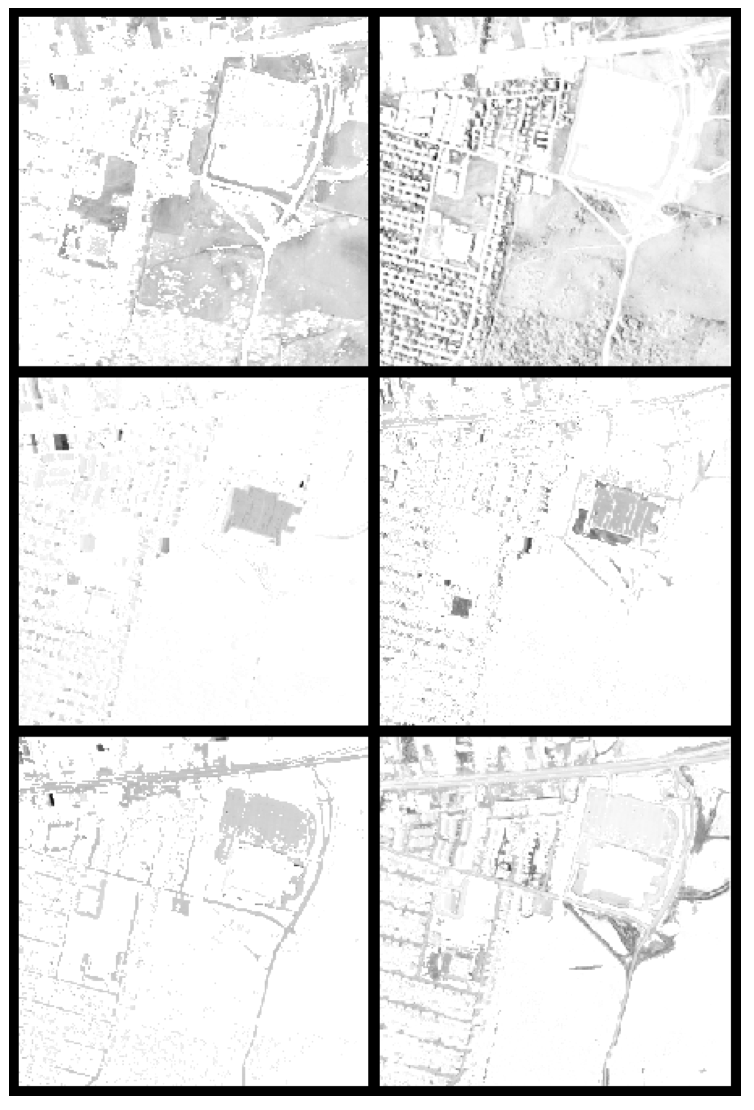
\includegraphics[width=3.5cm]{img/sca.png}};
            \node[xshift=110,font=\small] at (0,2.75) {J. Cohen, N. Gillis (2019)};
            \node[xshift=110,font=\small,text width=0.3\linewidth,align=center] at (0,-3.25) {Extract material abundance map from hyperspectral image};
        \end{scope}
    \end{tikzpicture}
\end{frame}

\begin{frame}{Context -- Operation research application}
    \begin{tikzpicture}

        % Define the coordinates of the nodes for reuse
        \coordinate (A) at (0,0);
        \coordinate (B) at (2,0);
        \coordinate (C) at (1,2);
        \coordinate (D) at (1,-2);
        \coordinate (E) at (3,1);
        \coordinate (F) at (3,-1);
        \coordinate (G) at (-1,1.5);
        \coordinate (H) at (-1,-1.5);
        \coordinate (I) at (4,0);
        \coordinate (J) at (-2,0);
      
        % Draw the first pane with nodes only
        \begin{scope}[scale=0.75]
          \node[ultra thick, circle, draw, minimum size=6mm] (A) at (0,0) {};
          \node[ultra thick, circle, draw, minimum size=6mm] (B) at (2,0) {};
          \node[ultra thick, circle, draw, minimum size=6mm, TolLightRed] (C) at (1,2) {\small\textcolor{TolLightRed}{\textbf{3}}};
          \node[ultra thick, circle, draw, minimum size=6mm, TolLightRed] (D) at (1,-2) {\small\textcolor{TolLightRed}{\textbf{3}}};
          \node[ultra thick, circle, draw, minimum size=6mm] (E) at (3,1) {};
          \node[ultra thick, circle, draw, minimum size=6mm] (F) at (3,-1) {};
          \node[ultra thick, circle, draw, minimum size=6mm] (G) at (-1,1.5) {};
          \node[ultra thick, circle, draw, minimum size=6mm] (H) at (-1,-1.5) {};
          \node[ultra thick, circle, draw, minimum size=6mm, TolLightRed] (I) at (4,0) {\small\textcolor{TolLightRed}{\textbf{3}}};
          \node[ultra thick, circle, draw, minimum size=6mm, TolLightBlue] (J) at (-2,0) {};
    
          \draw[ultra thick] (A) -- (B);
          \draw[ultra thick] (A) -- (C);
          \draw[ultra thick] (A) -- (D);
          \draw[ultra thick] (A) -- (G);
          \draw[ultra thick] (A) -- (H);
          \draw[ultra thick] (B) -- (C);
          \draw[ultra thick] (B) -- (D);
          \draw[ultra thick] (B) -- (E);
          \draw[ultra thick] (B) -- (F);
          \draw[ultra thick] (B) -- (I);
          \draw[ultra thick] (C) -- (E);
          \draw[ultra thick] (C) -- (G);
          \draw[ultra thick] (D) -- (F);
          \draw[ultra thick] (D) -- (H);
          \draw[ultra thick] (E) -- (I);
          \draw[ultra thick] (F) -- (I);
          \draw[ultra thick] (G) -- (H);
          \draw[ultra thick] (G) -- (J);
          \draw[ultra thick] (H) -- (J);
          \draw[ultra thick] (I) -- (E);
    
          \node[text width=0.5\linewidth,align=center] at (1,3.5) {Max. capacity per edge: 10 \\ Edge construction cost: 5};
          \node[text width=0.5\linewidth,align=center] at (1,-3.5) {Which edges to build to transport flows from \textcolor{TolLightBlue}{source} to \textcolor{TolLightRed}{sink} nodes ?};

          \node[text width=0.35\linewidth,align=center] at (9,1) {
            \begin{blockcolor}{mDarkTeal}{Network design}
                \centering
                $\textstyle
                \left\{
                    \begin{array}{rl}
                        \min & Q(\pv) + \reg\norm{\pv}{0} \\ 
                        \text{s.t.} & \mathbf{D}\pv \leq \mathbf{d}, \ \pv \leq \mathbf{c} \\ & \pv \in \kR+^{\card(E)}
                    \end{array}
                \right.$
            \end{blockcolor}
          };
          \node[text width=0.5\linewidth,align=left] at (10.5,-2) {\begin{itemize}[nosep]\item[$Q$ :] transportation cost \item[$\reg$ :] unit construction cost \item[$\mathbf{D}\pv \leq \mathbf{d}$ :] flow conservation \item[$\pv \leq \mathbf{c}$ :] capacity constraint\end{itemize}};
        \end{scope}
    \end{tikzpicture}
\end{frame}

\begin{frame}{Context -- Signal processing application}
    \begin{tikzpicture}[remember picture,overlay]
        \begin{scope}[xshift=0.5\textwidth]
            \node at (0,3.5) {\textbf{Compressed sensing}};
            %
            \node[text width=0.25\linewidth,align=center] (groundtruth) at (-4,2.5) {Sparse signal \\ $\pv \in \kR^{\pdim}$};
            \node[text width=0.25\linewidth,align=center] (observation) at (4,2.5) {Observation \\ $\obs = \dic\pv + \boldsymbol{\epsilon} \in \kR^{\ddim}$};
            %
            \draw[ultra thick,->] ($(groundtruth.north east)+(0,-0.25)$) .. controls (0,3.25) .. ($(observation.north west)+(0,-0.25)$) node[midway,fill=TolLightWhite,draw,ultra thick,text width=0.35\linewidth,align=center,yshift=-5] {Linear measurement};
            \draw[ultra thick,<-] ($(groundtruth.south east)+(0,0.25)$) .. controls (0,1.75) .. ($(observation.south west)+(0,0.25)$) node[midway,fill=TolLightWhite,draw,ultra thick,text width=0.35\linewidth,align=center,yshift=5] {Recover $\pv$ from $\dic$ and $\obs$};
            %
            \draw ($(groundtruth)+(0,-1.75)$) node {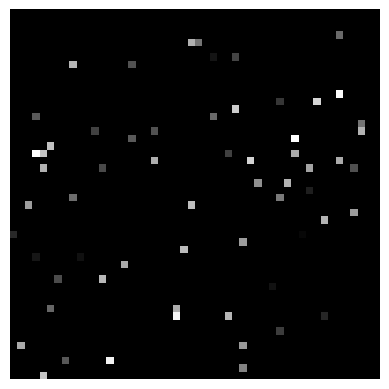
\includegraphics[width=2cm]{img/cs-x.png}};
            \draw ($(observation)+(0,-1.75)$) node {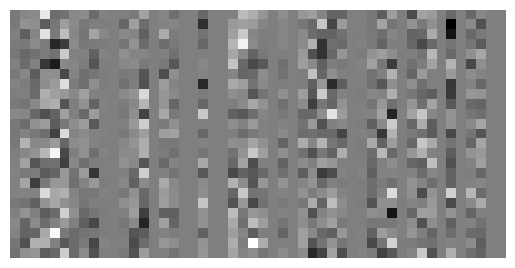
\includegraphics[width=2.5cm]{img/cs-y.png}};
            %
            \node [text width=0.45\textwidth] at (-3,-1) (problem) {
                \begin{blockcolor}{mDarkTeal}{Goal}
                    \centering
                    Find $\pv$ such that $\obs \simeq \dic\pv$
                \end{blockcolor}
            }; 
            %
            \node [text width=0.45\textwidth] at ($(problem)+(0,-2.25)$) (problem-sparse) {
                \begin{blockcolor}{mDarkTeal}{Goal (with sparse prior)}
                    \centering
                    Find $\pv$ \textcolor{TolLightOrange}{sparse} such that $\obs \simeq \dic\pv$
                \end{blockcolor}
            };
            %
            \draw[ultra thick,->] ($(problem)+(0,-0.75)$) -- ($(problem-sparse)+(0,0.5)$) node[midway,fill=TolLightWhite,draw,ultra thick] {$\ddim \ll \pdim$ : no unique solution};
            %
            \node [text width=0.45\textwidth] at (3,-1) (problem) {
                \begin{blockcolor}{mDarkTeal}{Optimization problem}
                    \centering
                    $\min_{\pv \in \kR^{\pdim}} \tfrac{1}{2}\norm{\obs - \dic\pv}{2}^2$
                \end{blockcolor}
            }; 
            %
            \node [text width=0.45\textwidth] at ($(problem)+(0,-2.25)$) (problem-sparse) {
                \begin{blockcolor}{mDarkTeal}{Sparse optimization problem}
                    \centering
                    $\min_{\pv \in \kR^{\pdim}} \tfrac{1}{2}\norm{\obs - \dic\pv}{2}^2 + \textcolor{TolLightOrange}{\reg\norm{\pv}{0}}$
                \end{blockcolor}
            };
            %
            \draw[ultra thick,->] ($(problem)+(0,-0.75)$) -- ($(problem-sparse)+(0,0.5)$) node[midway,fill=TolLightWhite,draw,ultra thick] {sparsity-inducing function};
        \end{scope}
    \end{tikzpicture}
\end{frame}

\begin{frame}{Context -- Balancing solution quality and problem hardness}
    \begin{tikzpicture}[remember picture,overlay]
        \begin{scope}[xshift=0.5\textwidth]
            \node (dataset) at (0,2.5) {
                \scriptsize
                \begin{tabular}{c|cccccc|c}
                    \multicolumn{8}{c}{\small{Riboflavin dataset - P. Bühlmann \textit{et al.} (2014)}} \\
                    \toprule
                    Colony & AADK & AAPA & ABFA & ABH & ... & ZUR & \textbf{B2 prod.} \\
                    \midrule
                    \#1 & 8.49 & 8.11 & 8.32 & 10.28 & ... & 7.42 & \textbf{-6.64} \\
                    \#2 & 7.29 & 6.39 & 11.32 & 9.42 & ... & 6.99 & \textbf{-5.43} \\
                    ... & ... & ... & ... & ... & ... & ... & ... \\
                    \#71 & 6.85 & 8.27 & 7.98 & 8.04 & ... & 6.65 & \textbf{-7.58} \\
                    \bottomrule
                \end{tabular}
            };
            %
            \draw[ultra thick,-] ($(dataset.south)+(-2.4,0)$) -- ($(dataset.south)+(-2.4,-0.05)$) -- ($(dataset.south)+(2.15,-0.05)$) node[midway,below,font=\small] {4,088 genes} -- ($(dataset.south)+(2.15,0)$);
        \end{scope}
        %
        \begin{scope}[xshift=30,yshift=-80]
            \pgfplotscreateplotcyclelist{cycle_quality_hardness}{
                TolLightBlue, very thick, mark=*, mark options={scale=0.5}\\
                TolLightGreen, very thick, mark=*, mark options={scale=0.5}\\
                TolLightBrown, very thick, mark=*, mark options={scale=0.5}\\    
                TolLightRed, very thick, mark=*, mark options={scale=0.5}\\
            }
            \begin{groupplot}[
                group style={
                    group size=2 by 1,
                    horizontal sep=0.2\textwidth,
                },
                width   = 0.48\textwidth,
                height  = 0.4\textwidth,
                xlabel  = \textbf{Number of genes},
                legend columns=5, 
                legend style={
                    at={(-0.35,1)},
                    anchor=south,
                    /tikz/every even column/.style = {column sep=5pt},
                    draw=none,
                },
                cycle list name=cycle_quality_hardness,
                mbaseplot,
                axis line style = ultra thick,
                major tick style = {ultra thick,color=mDarkTeal},
                minor tick style={draw=none},
                xmajorgrids=true,
                ymajorgrids=true,
                major grid style={dotted},
                axis x line=bottom,
                axis y line=left,
            ]

                \nextgroupplot[
                    ylabel = \textbf{Model error},
                    ymode=log,
                    ymin=0.09,
                    ymax=1.5,
                ]
                \foreach \method in {omp,lasso,enet,el0ps} {
                    \addplot table[x=nnz_grid,y=\method_test_error,col sep=comma]{data/riboflavin_quality.csv};
                }

                \nextgroupplot[
                    ymode=log,
                    ylabel = \textbf{Time (sec.)},
                    ytick={0.001,0.01,0.1,1,10,100},
                    ymax=70,
                    ymin=0.0004,
                ]
                \foreach \method in {omp,lasso,enet,el0ps} {
                    \addplot table[x=nnz_grid,y=\method_solve_time,col sep=comma]{data/riboflavin_quality.csv};
                }

                \addlegendentry{Omp (sklearn)};
                \addlegendentry{Lasso (sklearn)};
                \addlegendentry{E-Net (sklearn)};
                \addlegendentry{$\ell_0$-prob. (el0ps)};
            \end{groupplot}
        \end{scope}
    \end{tikzpicture}
\end{frame}

\begin{frame}{Context -- Balancing solution quality and problem hardness}
    \begin{tikzpicture}[remember picture,overlay]
        \begin{scope}[xshift=0.5\textwidth]
            \node[text width=0.25\linewidth,align=center] (groundtruth) at (-5,2.75) {Sparse signal \\ $\pv \in \kR^{\pdim}$};
            \node[text width=0.25\linewidth,align=center] (observation) at (-1,2.75) {Observation \\ $\obs = \dic\pv + \boldsymbol{\epsilon} \in \kR^{\ddim}$};
            %
            \draw[ultra thick,->] ($(groundtruth.north east)+(0,-0.25)$) .. controls (-3,3.5) .. ($(observation.north west)+(0,-0.25)$);
            \draw[ultra thick,<-] ($(groundtruth.south east)+(0,0.25)$) .. controls (-3,2) .. ($(observation.south west)+(0,0.25)$);
            %
            \node[text width=0.6\linewidth,align=center,font=\small] at (-3,1) {\textbf{Setup} \\ $\dic \in \kR^{100\times200}$ highly correlated, $\boldsymbol{\epsilon} \sim \mathcal{N}(0,\sigma\mathbf{I})$, \\ $\pv$ with 10 unit spikes of random location};
        \end{scope}
        %
        \begin{scope}[xshift=205,yshift=30]
            \pgfplotscreateplotcyclelist{cycle_quality_hardness}{
                TolLightBlue, very thick, mark=*, mark options={scale=0.5}\\
                TolLightGreen, very thick, mark=*, mark options={scale=0.5}\\
                TolLightBrown, very thick, mark=*, mark options={scale=0.5}\\    
                TolLightRed, very thick, mark=*, mark options={scale=0.5}\\
            }
            \begin{groupplot}[
                group style={
                    group size=1 by 1,
                    horizontal sep=0.2\textwidth,
                },
                width   = 0.48\textwidth,
                height  = 0.4\textwidth,
                xlabel  = \textbf{Number of non-zeros},
                legend columns=5, 
                legend style={
                    at={(-0.35,1)},
                    anchor=south,
                    /tikz/every even column/.style = {column sep=5pt},
                    draw=none,
                },
                cycle list name=cycle_quality_hardness,
                mbaseplot,
                axis line style = ultra thick,
                major tick style = {ultra thick,color=mDarkTeal},
                minor tick style={draw=none},
                xmajorgrids=true,
                ymajorgrids=true,
                major grid style={dotted},
                axis x line=bottom,
                axis y line=left,
            ]
                \nextgroupplot[
                    ylabel = \textbf{F1-score},
                    ymin=-0.1,
                    ymax=1.1,
                ]
                    \foreach \method in {omp,lasso,enet,proposed} {
                        \addplot table[x=nnz_grid,y=\method_f1_score,col sep=comma]{data/statistics_random_unit.csv};
                    }
            \end{groupplot}
        \end{scope}
        %
        \begin{scope}[xshift=25,yshift=-95]
            \pgfplotscreateplotcyclelist{cycle_quality_hardness}{
                TolLightBlue, very thick, mark=*, mark options={scale=0.5}\\
                TolLightGreen, very thick, mark=*, mark options={scale=0.5}\\
                TolLightBrown, very thick, mark=*, mark options={scale=0.5}\\    
                TolLightRed, very thick, mark=*, mark options={scale=0.5}\\
            }
            \begin{groupplot}[
                group style={
                    group size=2 by 1,
                    horizontal sep=0.25\textwidth,
                },
                width   = 0.48\textwidth,
                height  = 0.4\textwidth,
                xlabel  = \textbf{Num. of non-zeros},
                legend columns=5, 
                legend style={
                    at={(-0.35,1)},
                    anchor=south,
                    /tikz/every even column/.style = {column sep=5pt},
                    draw=none,
                },
                cycle list name=cycle_quality_hardness,
                mbaseplot,
                axis line style = ultra thick,
                major tick style = {ultra thick,color=mDarkTeal},
                minor tick style={draw=none},
                xmajorgrids=true,
                ymajorgrids=true,
                major grid style={dotted},
                axis x line=bottom,
                axis y line=left,
            ]

                \nextgroupplot[
                    ylabel = \textbf{Model error},
                    ymode=log,
                    ymin=0.09,
                    ymax=1.5,
                ]
                \foreach \method in {omp,lasso,enet,proposed} {
                    \addplot table[x=nnz_grid,y=\method_test_error,col sep=comma]{data/statistics_random_unit.csv};
                }

                \nextgroupplot[
                    ymode=log,
                    ylabel = \textbf{Time (sec.)},
                    ytick={0.001,0.01,0.1,1,10,100},
                    ymax=70,
                    ymin=0.0004,
                ]
                \foreach \method in {omp,lasso,enet,proposed} {
                    \addplot table[x=nnz_grid,y=\method_solve_time,col sep=comma]{data/statistics_random_unit.csv};
                }

                \addlegendentry{Omp (sklearn)};
                \addlegendentry{Lasso (sklearn)};
                \addlegendentry{E-Net (sklearn)};
                \addlegendentry{$\ell_0$-prob. (el0ps)};
            \end{groupplot}
        \end{scope}
    \end{tikzpicture}
\end{frame}

\begin{frame}{Context -- Balancing solution quality and problem hardness}
    \begin{tikzpicture}[remember picture,overlay]
        \begin{scope}[xshift=0.5\textwidth]
            \node[text width=0.25\linewidth,align=center] (groundtruth) at (-5,2.75) {Sparse signal \\ $\pv \in \kR^{\pdim}$};
            \node[text width=0.25\linewidth,align=center] (observation) at (-1,2.75) {Observation \\ $\obs = \dic\pv + \boldsymbol{\epsilon} \in \kR^{\ddim}$};
            %
            \draw[ultra thick,->] ($(groundtruth.north east)+(0,-0.25)$) .. controls (-3,3.5) .. ($(observation.north west)+(0,-0.25)$);
            \draw[ultra thick,<-] ($(groundtruth.south east)+(0,0.25)$) .. controls (-3,2) .. ($(observation.south west)+(0,0.25)$);
            %
            \node[text width=0.6\linewidth,align=center,font=\small] at (-3,1) {\textbf{Setup} \\ $\dic \in \kR^{100\times200}$ highly correlated, $\boldsymbol{\epsilon} \sim \mathcal{N}(0,\sigma\mathbf{I})$, \\ $\pv$ with 10 unit and evenly-spaced spikes};
        \end{scope}
        %
        \begin{scope}[xshift=205,yshift=30]
            \pgfplotscreateplotcyclelist{cycle_quality_hardness}{
                TolLightBlue, very thick, mark=*, mark options={scale=0.5}\\
                TolLightGreen, very thick, mark=*, mark options={scale=0.5}\\
                TolLightBrown, very thick, mark=*, mark options={scale=0.5}\\    
                TolLightRed, very thick, mark=*, mark options={scale=0.5}\\
            }
            \begin{groupplot}[
                group style={
                    group size=1 by 1,
                    horizontal sep=0.2\textwidth,
                },
                width   = 0.48\textwidth,
                height  = 0.4\textwidth,
                xlabel  = \textbf{Num. of non-zeros},
                legend columns=5, 
                legend style={
                    at={(-0.35,1)},
                    anchor=south,
                    /tikz/every even column/.style = {column sep=5pt},
                    draw=none,
                },
                cycle list name=cycle_quality_hardness,
                mbaseplot,
                axis line style = ultra thick,
                major tick style = {ultra thick,color=mDarkTeal},
                minor tick style={draw=none},
                xmajorgrids=true,
                ymajorgrids=true,
                major grid style={dotted},
                axis x line=bottom,
                axis y line=left,
            ]
                \nextgroupplot[
                    ylabel = \textbf{F1-score},
                    ymin=-0.1,
                    ymax=1.1,
                ]
                    \foreach \method in {omp,lasso,enet,proposed} {
                        \addplot table[x=nnz_grid,y=\method_f1_score,col sep=comma]{data/statistics_2outof3_unit.csv};
                    }
            \end{groupplot}
        \end{scope}
        %
        \begin{scope}[xshift=25,yshift=-95]
            \pgfplotscreateplotcyclelist{cycle_quality_hardness}{
                TolLightBlue, very thick, mark=*, mark options={scale=0.5}\\
                TolLightGreen, very thick, mark=*, mark options={scale=0.5}\\
                TolLightBrown, very thick, mark=*, mark options={scale=0.5}\\    
                TolLightRed, very thick, mark=*, mark options={scale=0.5}\\
            }
            \begin{groupplot}[
                group style={
                    group size=2 by 1,
                    horizontal sep=0.25\textwidth,
                },
                width   = 0.48\textwidth,
                height  = 0.4\textwidth,
                xlabel  = \textbf{Num. of non-zeros},
                legend columns=5, 
                legend style={
                    at={(-0.35,1)},
                    anchor=south,
                    /tikz/every even column/.style = {column sep=5pt},
                    draw=none,
                },
                cycle list name=cycle_quality_hardness,
                mbaseplot,
                axis line style = ultra thick,
                major tick style = {ultra thick,color=mDarkTeal},
                minor tick style={draw=none},
                xmajorgrids=true,
                ymajorgrids=true,
                major grid style={dotted},
                axis x line=bottom,
                axis y line=left,
            ]

                \nextgroupplot[
                    ylabel = \textbf{Model error},
                    ymode=log,
                    ymin=0.09,
                    ymax=1.5,
                ]
                \foreach \method in {omp,lasso,enet,proposed} {
                    \addplot table[x=nnz_grid,y=\method_test_error,col sep=comma]{data/statistics_2outof3_unit.csv};
                }

                \nextgroupplot[
                    ymode=log,
                    ylabel = \textbf{Time (sec.)},
                    ytick={0.001,0.01,0.1,1,10,100},
                    ymax=70,
                    ymin=0.0004,
                ]
                \foreach \method in {omp,lasso,enet,proposed} {
                    \addplot table[x=nnz_grid,y=\method_solve_time,col sep=comma]{data/statistics_2outof3_unit.csv};
                }

                \addlegendentry{Omp (sklearn)};
                \addlegendentry{Lasso (sklearn)};
                \addlegendentry{E-Net (sklearn)};
                \addlegendentry{$\ell_0$-prob. (el0ps)};
            \end{groupplot}
        \end{scope}
    \end{tikzpicture}
\end{frame}

\begin{frame}{Context -- A bit of history}
    \begin{tikzpicture}[remember picture,overlay]
        \begin{scope}[xshift=0.5\textwidth]
            \node[align=center,text width=0.35\textwidth] (problem) at (0,3) {
                \begin{blockcolor}{mDarkTeal}{Problem}
                    \centering
                    $\min_{\pv \in \kR^{\pdim}} \lfunc(\dic\pv) + \reg\norm{\pv}{0}$
                \end{blockcolor}
            };
            %
            \node (linecenter) at ($(current page.north)+(0,-0.5\textheight)$) {};
            \draw [ultra thick,->] ($(linecenter)+(-6,0)$) -- ($(linecenter)+(6,0)$) node (arrow) [midway] {};
            %
            \node (date1) at ($(linecenter)+(-5,0)$) {};
            \draw [ultra thick,-] ($(date1)+(0,-0.02\textheight)$) -- ($(date1)+(0,0.02\textheight)$);
            \node at ($(date1)+(0,+0.06\textheight)$)  {\textbf{1995}};
            \node[text width=0.2\textwidth,align=center,font=\small] at ($(date1)+(0,-0.05\textheight)$) {Heuristics};
            \node[text width=0.3\textwidth,align=center,font=\scriptsize] at ($(date1)+(0,-0.12\textheight)$) {MP, OMP, ... \\ S. Mallat (1993)};
            %
            \node (origin1) at ($(date1)+(0,-0.4\textheight)$) {};
            \fill[draw,thick,fill=TolLightWhite] ($(origin1)+(-0.5,0)$) circle (0.1);
            \fill[draw,thick,fill=TolLightOrange] ($(origin1)+(-0.5,0.3)$) circle (0.1);
            \fill[draw,thick,fill=TolLightWhite] ($(origin1)+(-0.5,0.6)$) circle (0.1);
            \fill[draw,thick,fill=TolLightWhite] ($(origin1)+(-0.5,0.9)$) circle (0.1);
            \fill[draw,thick,fill=TolLightWhite] ($(origin1)+(-0.5,1.2)$) circle (0.1);
            \fill[draw,thick,fill=TolLightWhite] ($(origin1)+(-0.5,1.5)$) circle (0.1);
            \node at ($(origin1)+(-0.5,-0.4)$) {$\pv^1$};
            %
            \fill[draw,thick,fill=TolLightWhite] ($(origin1)+(0,0)$) circle (0.1);
            \fill[draw,thick,fill=TolLightOrange] ($(origin1)+(0,0.3)$) circle (0.1);
            \fill[draw,thick,fill=TolLightWhite] ($(origin1)+(0,0.6)$) circle (0.1);
            \fill[draw,thick,fill=TolLightOrange] ($(origin1)+(0,0.9)$) circle (0.1);
            \fill[draw,thick,fill=TolLightWhite] ($(origin1)+(0,1.2)$) circle (0.1);
            \fill[draw,thick,fill=TolLightWhite] ($(origin1)+(0,1.5)$) circle (0.1);
            \node at ($(origin1)+(0,-0.4)$) {$\pv^2$};
            %
            \fill[draw,thick,fill=TolLightWhite] ($(origin1)+(0.5,0)$) circle (0.1);
            \fill[draw,thick,fill=TolLightOrange] ($(origin1)+(0.5,0.3)$) circle (0.1);
            \fill[draw,thick,fill=TolLightWhite] ($(origin1)+(0.5,0.6)$) circle (0.1);
            \fill[draw,thick,fill=TolLightOrange] ($(origin1)+(0.5,0.9)$) circle (0.1);
            \fill[draw,thick,fill=TolLightOrange] ($(origin1)+(0.5,1.2)$) circle (0.1);
            \fill[draw,thick,fill=TolLightWhite] ($(origin1)+(0.5,1.5)$) circle (0.1);
            \node at ($(origin1)+(0.5,-0.4)$) {$\pv^3$};
            %
            %
            %
            \node (date2) at ($(linecenter)+(-2.5,0)$) {};
            \draw [ultra thick,-] ($(date2)+(0,-0.02\textheight)$) -- ($(date2)+(0,0.02\textheight)$);
            \node at ($(date2)+(0,+0.06\textheight)$)  {\textbf{2000}};
            \node[text width=0.25\textwidth,align=center,font=\small] at ($(date2)+(0,-0.053\textheight)$) {Recovery cond.};
            \node[text width=0.3\textwidth,align=center,font=\scriptsize] at ($(date2)+(0,-0.12\textheight)$) {RIP, NSP, ... \\ E. Candes (2004)};
            %
            \node (origin2) at ($(date2)+(0,-0.4\textheight)$) {};
            \node[text width=0.2\linewidth,align=center] at ($(origin2)+(0,0.05\textheight)$) {OMP solves $\ell_0$-problem under RIP};
            %
            %
            %
            \node (date3) at ($(linecenter)+(0,0)$) {};
            \draw [ultra thick,-] ($(date3)+(0,-0.02\textheight)$) -- ($(date3)+(0,0.02\textheight)$);
            \node at ($(date3)+(0,+0.06\textheight)$)  {\textbf{2005}};
            \node[font=\small] at ($(date3)+(0,-0.053\textheight)$) {Convex approx.};
            \node[text width=0.3\textwidth,align=center,font=\scriptsize] at ($(date3)+(0,-0.12\textheight)$) {Lasso, Elastic-Net, ... \\ R. Tibshirani (2005)};
            %
            \node (origin3) at ($(date3)+(0,-0.4\textheight)$) {};
            \draw[ultra thick,->] ($(origin3)+(-1,0)$) -- ($(origin3)+(1, 0)$);
            \draw[ultra thick,->] ($(origin3)+(0,0)$) -- ($(origin3)+(0,1.5)$);
            \draw[-,very thick,TolLightOrange] ($(origin3)+(-0.05,0.8)$) -- ($(origin3)+(-1,0.8)$);
            \draw[-,very thick,TolLightOrange] ($(origin3)+(0.05,0.8)$) -- ($(origin3)+(1,0.8)$);
            \draw[very thick,dashed,TolLightOrange] (origin3) .. controls ($(origin3)+(-0.5,0.1)$) ..  ($(origin3)+(-1,0.8)$);
            \draw[very thick,dashed,TolLightOrange] (origin3) .. controls ($(origin3)+(0.5,0.1)$) ..  ($(origin3)+(1,0.8)$);
            \draw[TolLightOrange,very thick] ($(origin3)+(0,0.8)$) circle (0.075);
            \fill[TolLightOrange] (origin3) circle (0.075);
            %
            %
            %
            \node (date4) at ($(linecenter)+(2.5,0)$) {};
            \draw [ultra thick,-] ($(date4)+(0,-0.02\textheight)$) -- ($(date4)+(0,0.02\textheight)$);
            \node at ($(date4)+(0,+0.06\textheight)$)  {\textbf{2010}};
            \node[font=\small] at ($(date4)+(0,-0.053\textheight)$) {Concave approx.};
            \node[text width=0.3\textwidth,align=center,font=\scriptsize] at ($(date4)+(0,-0.12\textheight)$) {SCAD, MCP, ... \\ C. Zhang (2010)};
            %
            \node (origin4) at ($(date4)+(0,-0.4\textheight)$) {};
            \draw[ultra thick,->] ($(origin4)+(-1,0)$) -- ($(origin4)+(1, 0)$);
            \draw[ultra thick,->] ($(origin4)+(0,0)$) -- ($(origin4)+(0,1.5)$);
            \draw[-,very thick,TolLightOrange] ($(origin4)+(-0.05,0.8)$) -- ($(origin4)+(-1,0.8)$);
            \draw[-,very thick,TolLightOrange] ($(origin4)+(0.05,0.8)$) -- ($(origin4)+(1,0.8)$);
            \draw[very thick,TolLightOrange,dashed] (origin4) .. controls ($(origin4)+(-0.5,0.8)$) ..  ($(origin4)+(-1,0.8)$);
            \draw[very thick,TolLightOrange,dashed] (origin4) .. controls ($(origin4)+(0.5,0.8)$) ..  ($(origin4)+(1,0.8)$);
            \draw[TolLightOrange,very thick] ($(origin4)+(0,0.8)$) circle (0.075);
            \fill[TolLightOrange] (origin4) circle (0.075);
            %
            %
            %
            \node (date5) at ($(linecenter)+(5,0)$) {};
            \draw[ultra thick,-] ($(date5)+(0,-0.02\textheight)$) -- ($(date5)+(0,0.02\textheight)$);
            \node at ($(date5)+(0,+0.06\textheight)$)  {\textbf{2015}};
            \node[text width=0.22\textwidth,align=center,font=\small,TolLightOrange] at ($(date5)+(0,-0.05\textheight)$) {Exact methods};
            \node[text width=0.3\textwidth,align=center,font=\scriptsize] at ($(date5)+(0,-0.12\textheight)$) {MIP, BnB, ... \\ D. Bertsimas (2016)};
            %
            \node (origin5) at ($(date5)+(0,-0.4\textheight)$) {};
            \draw[ultra thick,->] ($(origin5)+(-1,0)$) -- ($(origin5)+(1, 0)$);
            \draw[ultra thick,->] ($(origin5)+(0,0)$) -- ($(origin5)+(0,1.5)$);
            \draw[-,very thick,TolLightOrange] ($(origin5)+(-0.05,0.8)$) -- ($(origin5)+(-1,0.8)$);
            \draw[-,very thick,TolLightOrange] ($(origin5)+(0.05,0.8)$) -- ($(origin5)+(1,0.8)$);
            \draw[TolLightOrange,very thick] ($(origin5)+(0,0.8)$) circle (0.075);
            \fill[TolLightOrange] (origin5) circle (0.075);
        \end{scope}
    \end{tikzpicture}
\end{frame}

\begin{frame}{Context -- MIP formulation}
    \begin{tikzpicture}[remember picture,overlay]
        \begin{scope}[xshift=0.5\textwidth]
            \node[align=center,text width=0.5\textwidth] (problem) at (-2.5,3.25) {
                \begin{blockcolor}{mDarkTeal}{Problem}
                    \centering
                    $\min_{\pv \in \kR^{\pdim}} \lfunc(\dic\pv) + \reg\norm{\pv}{0} + \pfunc(\pv)$
                \end{blockcolor}
            };
            %
            \node[text width=0.5\linewidth,align=center,font=\small] at ($(problem)+(5.75,-0.15)$) {\textbf{Use generic MIP solvers} \\ Need standardized expressions \\ linear/quadratic/conic/...};
            %
            \node[align=center,text width=0.5\textwidth] (mip) at ($(problem)+(0,-2.9)$) {
                \begin{blockcolor}{mDarkTeal}{MIP formulation}
                    \centering
                    $\left\{\begin{array}{rcl}\min && \lfunc(\dic\pv) + \reg\textcolor{TolLightOrange}{\transp{\1}\bv} + \pfunc(\pv) \\
                    \text{s.t.} && \textcolor{TolLightOrange}{\pvi{\idxentry} = 0 \implies \bvi{\idxentry} = 0, \ \forall \idxentry} \\
                    && \pv \in \kR^{\pdim}, \ \bv \in \{0,1\}^{\pdim}\end{array}\right.$
                \end{blockcolor}
            };
            %
            \node[text width=0.4\linewidth,align=center,font=\small] at ($(mip)+(5.75,-0.15)$) {\textbf{Lifted formulation} \\ $\norm{\pv}{0}$ $=$ $\transp{\1}\bv$ \\ for all $\pv \in \kR^{\pdim}$ and $\bv \in \{0,1\}^{\pdim}$ \\ if $\pvi{\idxentry} = 0$ $\implies$ $\bvi{\idxentry} = 0, \ \forall \idxentry$};
            %
            \draw[ultra thick,->] (problem) -- ($(mip.north)+(0,-0.25)$) node[midway,font=\small,fill=TolLightWhite,draw,ultra thick] {linearize $\ell_0$-norm};
            %
            \node[align=center,text width=0.5\textwidth] (practical-mip) at ($(mip)+(0,-3.25)$) {
                \begin{blockcolor}{mDarkTeal}{Practical MIP formulation}
                    \centering
                    $\left\{\begin{array}{rcl}\min && \lfunc(\dic\pv) + \reg\transp{\1}\bv + \textcolor{TolLightOrange}{\pfunc_{\text{mip}}}(\pv,\bv) \\
                    \text{s.t.} && \pv \in \kR^{\pdim}, \ \bv \in \{0,1\}^{\pdim}\end{array}\right.$
                \end{blockcolor}
            };
            %
            \draw[ultra thick,->] (mip) -- ($(practical-mip.north)+(0,-0.25)$) node[midway,font=\small,fill=TolLightWhite,draw,ultra thick] {avoid logical cstr.};
            %
            \node[text width=0.5\linewidth,align=center,font=\small] at ($(practical-mip)+(5.75,-0.15)$) {
                \textbf{Construct $\pfunc_{\text{mip}}$ depending on $\pfunc$} \\ \begin{tabular}{c|c} $\pfunc(\pv)$ & $\pfunc_{\text{mip}}(\pv,\bv)$ \\ \toprule $\icvx(\norm{\pv}{\infty} \leq \bigM)$ & $\icvx(-\bigM\bv \leq \pv \leq \bigM\pv)$ \\ $\regtwo\norm{\pv}{2}^2$ & $\sum_{\idxentry=1}^{\pdim}\regtwo\tfrac{\pvi{\idxentry}^2}{\bvi{\idxentry}}$\end{tabular}
            };
        \end{scope}
    \end{tikzpicture}
\end{frame}

\begin{frame}{Context -- Research community}
    \begin{tikzpicture}[remember picture,overlay]
        \node[fill=TolLightOrange] at ($(current page.north)+(4.8,-1.3)$) {\textcolor{TolLightWhite}{Non-exhaustive list}};
        %
        \node[align=center,text width=0.3\linewidth] (usa) at ($(current page.center)+(-2.3,2)$) {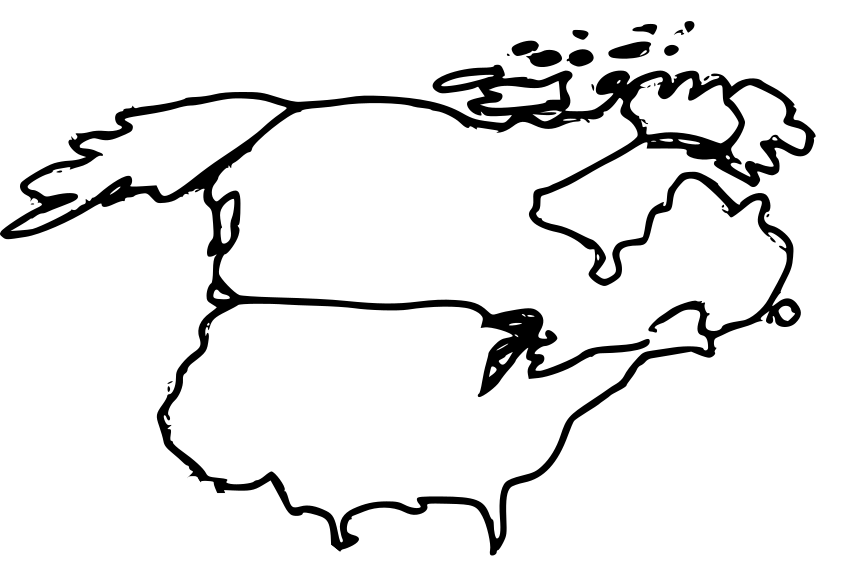
\includegraphics[width=1.5\textwidth]{img/usa.png}};
        %
        \draw[<-,ultra thick] ($(usa)+(1.9,-0.7)$) .. controls ($(usa)+(4.7,-0.4)$) .. ($(usa)+(5,0.1)$) node [above,align=center,font=\scriptsize] {\textbf{MIT}~\\ D. Bertsimas, R. Mazmuder, ...~\\\textit{MIO tools for $\ell_0$-problems}};
        %
        \draw[<-,ultra thick] ($(usa)+(0.25,0.45)$) .. controls ($(usa)+(-1.9,0.1)$) .. ($(usa)+(-2.3,-0.1)$) node [below,align=center,font=\scriptsize] {\textbf{Google Deep Mind}~\\ H. Hazimeh, A. Dedieu, ...~\\\textit{MIO-based heuristics and} \\ \textit{softwares}};
        %
        \draw[<-,ultra thick] ($(usa)+(-0.5,-1.2)$) .. controls ($(usa)+(-1.5,-1.4)$) .. ($(usa)+(-2,-1.9)$) node [below,align=center,font=\scriptsize] {\textbf{Berkley}~\\ A. Atamtürk, A. Gomès, ...~\\\textit{Convex-based acceleration}};
        %
        %
        %
        \node[align=center,text width=0.3\linewidth] (europe) at ($(current page.center)+(3.75,-2.5)$) {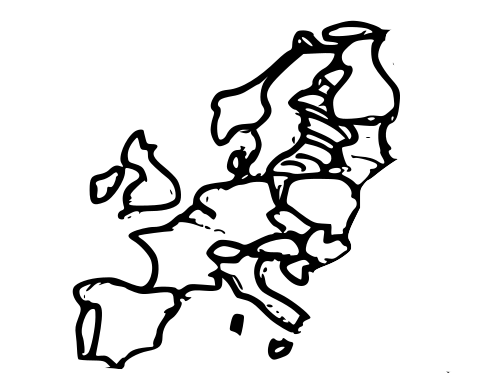
\includegraphics[width=1.5\textwidth]{img/europe.png}};
        %
        \draw[<-,ultra thick] ($(europe)+(0.7,1)$) .. controls ($(europe)+(0.5,1.5)$) .. ($(europe)+(1.1,3.5)$) node [above,align=center,font=\scriptsize] {\textbf{Lund University}~\\ M. Carlsson, C. Olsson...~\\\textit{Quadratic envelope}};
        %
        \draw[<-,ultra thick] ($(europe)+(0.4,0.1)$) .. controls ($(europe)+(-0.5,1.5)$) .. ($(europe)+(-1.2,2.5)$) node [above,align=center,font=\scriptsize] {\textbf{Frankfurt / Wurzburg Universities}~\\ C. Kanzow, A. Tillmann, ...~\\\textit{Optimality conditions}};
        %
        \draw[<-,ultra thick] ($(europe)+(-0.4,0.5)$) .. controls ($(europe)+(-1,1.3)$) .. ($(europe)+(-2,1.5)$) node [above left,align=center,font=\scriptsize] {\textbf{London Business School}~\\ J. Pauphilet, R. Cory-Wright, ...~\\\textit{Healthcare applications}};
        %
        \draw[<-,ultra thick] ($(europe)+(0.2,-0.6)$) .. controls ($(europe)+(-1.5,0.8)$) .. ($(europe)+(-2.5,0.9)$) node [left,align=center,font=\scriptsize] {\textbf{Ponts ParisTech}~\\ M. De Lara, P. Chancelier, A. Parmentier, ...~\\\textit{Non-convex analysis for $\ell_0$-norm, ML appli.}};
        %
        \draw[<-,ultra thick] ($(europe)+(-0.4,-0.4)$) .. controls ($(europe)+(-1,-0.4)$) .. ($(europe)+(-5,-0.2)$) node [left,align=center,font=\scriptsize] {\textbf{Centrale Nantes / ENSTA Bretagne}~\\ S. Bourguignon, J. Ninin, ...~\\\textit{Branch-and-Bound for $\ell_0$-problems}};
        %
        \draw[<-,ultra thick] ($(europe)+(-0.2,-0.7)$) .. controls ($(europe)+(-4,-0.7)$) .. ($(europe)+(-5.7,-0.9)$) node [below left,align=center,font=\scriptsize] {\textbf{Inria / CentraleSupélec}~\\ C. Herzet, C. Elvira, A. Arslan, ...~\\\textit{Generalization, acceleration}};
        %
        \draw[<-,ultra thick] ($(europe)+(0,-0.9)$) .. controls ($(europe)+(-0.5,-1.5)$) .. ($(europe)+(-1.7,-1.5)$) node [left,align=center,font=\scriptsize] {\textbf{IRIT / I3S}~\\ E. Soubies, L. Blanc-Féraud, ...~\\\textit{Strong relax. of $\ell_0$-norm}};
    \end{tikzpicture}
\end{frame}

\begin{frame}{BnB -- Region separation}
  \begin{tikzpicture}[remember picture,overlay]
    \begin{scope}[xshift=0.5\linewidth,scale=0.4]
        \node at (0,6) (node0) {};
        \fill[gray!60] ($(node0)+(-2,1.8)$) -- ($(node0)+(1.8,1.8)$) -- ($(node0)+(1.8,-2)$) -- ($(node0)+(-2,-2)$) -- ($(node0)+(-2,1.8)$);
        \draw[very thick, mDarkTeal, ->] ($(node0)+(-2.3,0)$) -- ($(node0)+(2.5,0)$) node[right] {\small$\pvi{1}$};
        \draw[very thick, mDarkTeal, ->] ($(node0)+(0,-2.3)$) -- ($(node0)+(0,2.5)$) node[above] {\small$\pvi{2}$};
        \node at ($(node0)+(-2.2,2.2)$) {$\kR^2$};
        %
        \node at ($(node0)+(7.5,-6)$) (node1) {};
        \fill[gray!60] ($(node1)+(-2,1.8)$) -- ($(node1)+(-0.3,1.8)$) -- ($(node1)+(-0.3,-2)$) -- ($(node1)+(-2,-2)$) -- ($(node1)+(-2,1.8)$);
        \fill[gray!60] ($(node1)+(1.8,1.8)$) -- ($(node1)+(0.3,1.8)$) -- ($(node1)+(0.3,-2)$) -- ($(node1)+(1.8,-2)$) -- ($(node1)+(1.8,1.8)$);
        \draw[very thick, mDarkTeal, ->] ($(node1)+(-2.3,0)$) -- ($(node1)+(2.5,0)$) node[right] {\small$\pvi{1}$};
        \draw[very thick, mDarkTeal, ->] ($(node1)+(0,-2.3)$) -- ($(node1)+(0,2.5)$) node[above] {\small$\pvi{2}$};
        %
        \node at ($(node0)+(-7.5,-6)$) (node2) {};
        \fill[gray!60] ($(node2)+(-0.3,1.8)$) -- ($(node2)+(0.3,1.8)$) -- ($(node2)+(0.3,-2)$) -- ($(node2)+(-0.3,-2)$) -- ($(node2)+(-0.3,1.8)$);
        \draw[very thick, mDarkTeal, ->] ($(node2)+(-2.3,0)$) -- ($(node2)+(2.5,0)$) node[right] {\small$\pvi{1}$};
        \draw[very thick, mDarkTeal, ->] ($(node2)+(0,-2.3)$) -- ($(node2)+(0,2.5)$) node[above] {\small$\pvi{2}$};
        %
        \draw[very thick,dashed,->] ($(node0)+(0,-3)$) .. controls ($(node0)+(0,-5)$) .. ($(node1)+(-4,1)$);
        \draw[very thick,dashed,->] ($(node0)+(0,-3)$) .. controls ($(node0)+(0,-5)$) .. ($(node2)+(4,1)$);
        %
        \node at ($(node2)+(-4,-6)$) (node3) {};
        \fill[gray!60] ($(node3)+(0.3,0.3)$) -- ($(node3)+(-0.3,0.3)$) -- ($(node3)+(-0.3,-0.3)$) -- ($(node3)+(0.3,-0.3)$) -- ($(node3)+(0.3,0.3)$);
        \draw[very thick, mDarkTeal, ->] ($(node3)+(-2.3,0)$) -- ($(node3)+(2.5,0)$) node[right] {\small$\pvi{1}$};
        \draw[very thick, mDarkTeal, ->] ($(node3)+(0,-2.3)$) -- ($(node3)+(0,2.5)$) node[above] {\small$\pvi{2}$};
        %
        \node at ($(node2)+(4,-6)$) (node4) {};
        \fill[gray!60] ($(node4)+(0.3,-2)$) -- ($(node4)+(0.3,-0.3)$) -- ($(node4)+(-0.3,-0.3)$) -- ($(node4)+(-0.3,-2)$) -- ($(node4)+(0.3,-2)$);
        \fill[gray!60] ($(node4)+(0.3,1.8)$) -- ($(node4)+(0.3,0.3)$) -- ($(node4)+(-0.3,0.3)$) -- ($(node4)+(-0.3,1.8)$) -- ($(node4)+(0.3,1.8)$);
        \draw[very thick, mDarkTeal, ->] ($(node4)+(-2.3,0)$) -- ($(node4)+(2.5,0)$) node[right] {\small$\pvi{1}$};
        \draw[very thick, mDarkTeal, ->] ($(node4)+(0,-2.3)$) -- ($(node4)+(0,2.5)$) node[above] {\small$\pvi{2}$};
        %       
        \draw[very thick,dashed,->] ($(node2)+(0,-3)$) .. controls ($(node2)+(0,-4)$) .. ($(node3)+(2.2,2)$);
        \draw[very thick,dashed,->] ($(node2)+(0,-3)$) .. controls ($(node2)+(0,-4)$) .. ($(node4)+(-2.2,2)$);
        %
        \node at ($(node1)+(-4,-6)$) (node5) {};
        \fill[gray!60] ($(node5)+(2,0.3)$) -- ($(node5)+(0.3,0.3)$) -- ($(node5)+(0.3,-0.3)$) -- ($(node5)+(2,-0.3)$) -- ($(node5)+(2,0.3)$);
        \fill[gray!60] ($(node5)+(-2,0.3)$) -- ($(node5)+(-0.3,0.3)$) -- ($(node5)+(-0.3,-0.3)$) -- ($(node5)+(-2,-0.3)$) -- ($(node5)+(-2,0.3)$);
        \draw[very thick, mDarkTeal, ->] ($(node5)+(-2.3,0)$) -- ($(node5)+(2.5,0)$) node[right] {\small$\pvi{1}$};
        \draw[very thick, mDarkTeal, ->] ($(node5)+(0,-2.3)$) -- ($(node5)+(0,2.5)$) node[above] {\small$\pvi{2}$};
        %
        \node at ($(node1)+(4,-6)$) (node6) {};
        \fill[gray!60] ($(node6)+(0.3,-0.3)$) -- ($(node6)+(0.3,-2)$) -- ($(node6)+(2,-2)$) -- ($(node6)+(2,-0.3)$) -- ($(node6)+(0.3,-0.3)$);
        \fill[gray!60] ($(node6)+(-0.3,-0.3)$) -- ($(node6)+(-0.3,-2)$) -- ($(node6)+(-2,-2)$) -- ($(node6)+(-2,-0.3)$) -- ($(node6)+(-0.3,-0.3)$);
        \fill[gray!60] ($(node6)+(0.3,0.3)$) -- ($(node6)+(0.3,2)$) -- ($(node6)+(2,2)$) -- ($(node6)+(2,0.3)$) -- ($(node6)+(0.3,0.3)$);
        \fill[gray!60] ($(node6)+(-0.3,0.3)$) -- ($(node6)+(-0.3,2)$) -- ($(node6)+(-2,2)$) -- ($(node6)+(-2,0.3)$) -- ($(node6)+(-0.3,0.3)$);
        \draw[very thick, mDarkTeal, ->] ($(node6)+(-2.3,0)$) -- ($(node6)+(2.5,0)$) node[right] {\small$\pvi{1}$};
        \draw[very thick, mDarkTeal, ->] ($(node6)+(0,-2.3)$) -- ($(node6)+(0,2.5)$) node[above] {\small$\pvi{2}$};
        %       
        \draw[very thick,dashed,->] ($(node1)+(0,-3)$) .. controls ($(node1)+(0,-4)$) .. ($(node5)+(2.2,2)$);
        \draw[very thick,dashed,->] ($(node1)+(0,-3)$) .. controls ($(node1)+(0,-4)$) .. ($(node6)+(-2.2,2)$);
    \end{scope} 
  \end{tikzpicture}
\end{frame}

\begin{frame}{Axis 1 -- Relaxation construction}
    \begin{tikzpicture}[remember picture,overlay]
        \begin{scope}[xshift=0.5\textwidth]
            \node at (-3,3) (node) {};
            \draw[ultra thick,->] ($(node)+(0.5,0.6)$) -- ($(node)+(0.25,0.27)$);
            \draw[
                ultra thick,
                top color = white,
                bottom color = gray!60,
            ] (node) circle (10pt) node {$\nodeSymb$};
            %
            \node[text width=0.75\linewidth,align=left,font=\small] at ($(node)+(5,0)$) {Region $\nodeSymb \equiv (\setzero,\setone,\setnone)$ with $\begin{cases} \pvi{\idxentry} = 0 & \text{if } \idxentry \in \setzero \\ \pvi{\idxentry} \neq 0 & \text{if } \idxentry \in \setone \\ \pvi{\idxentry} \in \kR & \text{if } \idxentry \in \setnone\end{cases}$};
            %
            \node[text width=0.5\linewidth,align=center,font=\small] (restrict) at (-3.75,1.5) {\textbf{Restriction to region $\nodeSymb$} \\ $\node{\pobj} = \min_{\textcolor{TolLightOrange}{\pv \in \nodeSymb}} \lfunc(\dic\pv) + \rfunc(\pv)$};
            %
            \node[anchor=west,font=\small] at ($(restrict)+(2.75,-0.24)$) {with $\qquad \separable{\rfunc}{\idxentry}(\pvi{\idxentry}) = \reg\norm{\pvi{\idxentry}}{0} + \separable{\pfunc}{\idxentry}(\pvi{\idxentry})$};
            %
            \node[text width=0.5\linewidth,align=center,font=\small] (reform) at ($(restrict)+(0,-2.25)$) {\textbf{Restriction to region $\nodeSymb$} \\ $\node{\pobj} = \min_{\textcolor{TolLightOrange}{\pv \in \kR^{\pdim}}} \lfunc(\dic\pv) + \textcolor{TolLightOrange}{\node{\rfunc}}(\pv)$};
            %
            \draw[ultra thick,->] ($(restrict.south)+(0,0)$) -- ($(reform.north)+(0,0)$) node[midway,fill=TolLightWhite,draw,font=\small] {reformulation};
            %
            \node[anchor=west,font=\small] at ($(reform)+(2.75,-0.24)$) {with $\qquad \node{\separable{\rfunc}{\idxentry}}(\pvi{\idxentry}) = \begin{cases}\separable{\rfunc}{\idxentry}(\pvi{\idxentry}) + \icvx(\pvi{\idxentry} = 0) & \text{if } \idxentry \in \setzero \\ \separable{\rfunc}{\idxentry}(\pvi{\idxentry}) + \icvx(\pvi{\idxentry} \neq 0) & \text{if } \idxentry \in \setone \\ \separable{\rfunc}{\idxentry}(\pvi{\idxentry}) & \text{if } \idxentry \in \setnone \end{cases}$};
            %
            \node[text width=0.5\linewidth,align=center,font=\small] (relax) at ($(reform)+(0,-2.25)$) {\textbf{Relaxation for region $\nodeSymb$} \\ $\node{\pobj}_{\text{lb}} = \min_{\pv \in \kR^{\pdim}} \lfunc(\dic\pv) + \textcolor{TolLightOrange}{\node{\rfunc}_{\text{lb}}}(\pv)$};
            %
            \draw[ultra thick,->] ($(reform.south)+(0,0)$) -- ($(relax.north)+(0,0)$) node[midway,fill=TolLightWhite,draw,font=\small] {$\node{\rfunc}_{\text{lb}} \leq \rfunc$, $\node{\rfunc}_{\text{lb}}$ convex};
            %
            \node[anchor=west,font=\small] at ($(relax)+(2.75,-0.24)$) {with $\qquad \node{\separable{\rfunc}{\idxentry,\text{lb}}}(\pvi{\idxentry}) = \begin{cases}\icvx(\pvi{\idxentry} = 0) & \text{if } \idxentry \in \setzero \\ \separable{\pfunc}{\idxentry}(\pvi{\idxentry}) + \reg & \text{if } \idxentry \in \setone \\ \textcolor{TolLightOrange}{\separable{\rfunc}{\idxentry,\text{cvx}}}(\pvi{\idxentry}) & \text{if } \idxentry \in \setnone \end{cases}$};
        \end{scope}
    \end{tikzpicture}
\end{frame}

\begin{frame}{Axis 1 -- Graphical interpretation}
    \begin{tikzpicture}[remember picture,overlay]
        \begin{scope}[xshift=0.5\linewidth]
            \node (rfunc) at (-3.5,3) {$\rfunc(\pvi{}) = \reg\norm{\pvi{}}{0} + \pfunc(\pvi{})$};
            \node (rfunccvx) at (3,3) {$\rfunc_{\text{cvx}}(\pvi{}) = \begin{cases}\rslope\abs{\pvi{}} &\text{if } \abs{\pvi{}} \leq \rlimit \\ \reg + \pfunc(\pvi{}) & \text{otherwise}\end{cases}$};
            \draw[ultra thick,->] ($(rfunc.east)+(0.25,0)$) -- ($(rfunccvx.west)+(-0.25,0)$) node[midway,above,font=\small] {convexify};
        \end{scope}
      \begin{scope}[xshift=0.125\textwidth,yshift=-0.075\textheight]
        \node[above,font=\small] at (0,2) {$\pfunc(\pvi{}) = \icvx(\abs{\pvi{}} \leq \bigM)$};
        \node[above,LavenderBlush4,font=\small] at (-0.75,1.25) {$\rfunc$};
        \node[above,TolLightOrange,font=\small] at (-1.4,1.25) {$\rfunc_{\text{cvx}}$};
        %
        \draw[ultra thick,->] (-1.75,0) -- (1.75,0);
        \draw[ultra thick,->] (0,-0.2) -- (0,1.75);
        \node[above left,font=] at (0,0.5) {$\reg$};
        %
        \draw[LavenderBlush4,ultra thick] (-1,2) -- (-1,0.5) -- (-0.05,0.5);
        \draw[LavenderBlush4,ultra thick] (1,2) -- (1,0.5) -- (0.05,0.5);
        %
        \draw[TolLightOrange,ultra thick] (-1.05,2) -- (-1.05,0.5) -- (0,0) -- (1.05,0.5) -- (1.05,2);
        %
        \draw[very thick,dashed] (0,0) -- (2,1);
        \draw[very thick,dashed] (0.45,0.15) .. controls (0.45,0.1) .. (0.5,0) node[midway,right,font=\small,yshift=2pt] {$\rslope$};
        \draw[very thick,dashed] (1,0.5) -- (1,0) node[below] {$\rlimit$};
        %
        \fill[mDarkTeal] (1,0.5) circle (0.075);
        \fill[LavenderBlush4] (0,0) circle (0.075);
        \draw[LavenderBlush4,ultra thick] (0,0.5) circle (0.075);
      \end{scope}
      \begin{scope}[xshift=0.5\textwidth,yshift=-0.075\textheight]
        \node[above,font=\small] at (0,2) {$\pfunc(\pvi{}) = \pvi{}^2$};
        \node[above,LavenderBlush4,font=\small] at (-1,1.25) {$\rfunc$};
        \node[above,TolLightOrange,font=\small] at (-1,0.4) {$\rfunc_{\text{cvx}}$};
        %
        \draw[ultra thick,->] (-1.75,0) -- (1.75,0);
        \draw[ultra thick,->] (0,-0.2) -- (0,1.75);
        \node[above left,font=] at (0,0.5) {$\reg$};
        %
        \draw[domain=-1.75:-0.05,smooth,variable=\x,LavenderBlush4,ultra thick] plot ({\x}, {0.5 + 0.5*\x*\x});
        \draw[domain=0.05:1.75,smooth,variable=\x,LavenderBlush4,ultra thick] plot ({\x}, {0.5 + 0.5*\x*\x});
        %
        \draw[ultra thick,TolLightOrange] (0,0) -- (1,0.95);
        \draw[domain=1:1.75,smooth,variable=\x,TolLightOrange,ultra thick] plot ({\x}, {0.45 + 0.5*\x*\x});
        \draw[domain=-1.75:-1,smooth,variable=\x,TolLightOrange,ultra thick] plot ({\x}, {0.45 + 0.5*\x*\x});
        \draw[ultra thick,TolLightOrange] (-1,0.95) -- (0,0);
        %
        \draw[very thick,dashed] (0,0) -- (2,1.9);
        \draw[very thick,dashed] (0.3,0.32) .. controls (0.45,0.2) .. (0.5,0) node[midway,right,font=\small] {$\rslope$};
        \draw[very thick,dashed] (1,1) -- (1,0) node[below] {$\rlimit$};
        %
        \fill[mDarkTeal] (1,0.95) circle (0.075);
        \fill[LavenderBlush4] (0,0) circle (0.075);
        \draw[LavenderBlush4,ultra thick] (0,0.5) circle (0.075);
      \end{scope}
      \begin{scope}[xshift=0.875\textwidth,yshift=-0.075\textheight]
        \node[above,font=\small] at (0,2) {$\pfunc(\pvi{}) = \icvx(\abs{\pvi{}} \leq \bigM) + \abs{\pvi{}}$};
        \node[above,LavenderBlush4,font=\small] at (-0.75,1.25) {$\rfunc$};
        \node[above,TolLightOrange,font=\small] at (-1.4,1.25) {$\rfunc_{\text{cvx}}$};
        %
        \draw[ultra thick,->] (-1.75,0) -- (1.75,0);
        \draw[ultra thick,->] (0,-0.2) -- (0,1.75);
        \node[above left,font=] at (0,0.5) {$\reg$};
        %
        \draw[LavenderBlush4,ultra thick] (-1,2) -- (-1,0.75) -- (-0.05,0.5);
        \draw[LavenderBlush4,ultra thick] (1,2) -- (1,0.75) -- (0.05,0.5);
        %
        \draw[TolLightOrange,ultra thick] (-1.05,2) -- (-1.05,0.75) -- (0,0) -- (1.05,0.75) -- (1.05,2);
        %
        \draw[very thick,dashed] (0,0) -- (2,1.5);
        \draw[very thick,dashed] (0.3,0.2) .. controls (0.45,0.1) .. (0.5,0) node[midway,right,font=\small,yshift=2pt] {$\rslope$};
        \draw[very thick,dashed] (1,0.75) -- (1,0) node[below] {$\rlimit$};
        %
        \fill[mDarkTeal] (1,0.75) circle (0.075);
        \fill[LavenderBlush4] (0,0) circle (0.075);
        \draw[LavenderBlush4,ultra thick] (0,0.5) circle (0.075);
      \end{scope}
      \begin{scope}[xshift=0.25\textwidth,yshift=-0.45\textheight]
        \node[above,font=\small] at (0,2) {$\pfunc(\pvi{}) = \abs{\pvi{}}$};
        \node[above,LavenderBlush4,font=\small] at (-1,1) {$\rfunc$};
        \node[above,TolLightOrange,font=\small] at (-1,0.1) {$\rfunc_{\text{cvx}}$};
        %
        \draw[ultra thick,->] (-1.75,0) -- (1.75,0);
        \draw[ultra thick,->] (0,-0.2) -- (0,1.75);
        \node[above left,font=] at (0,0.5) {$\reg$};
        %
        \draw[ultra thick,LavenderBlush4] (-2,1.5) -- (-0.05,0.5);
        \draw[ultra thick,LavenderBlush4] (2,1.5) -- (0.05,0.5);
        %
        \draw[ultra thick,TolLightOrange] (-2,1) -- (0,0) -- (2,1);
        %
        \draw[very thick,dashed] (0.4,0.2) .. controls (0.45,0.1) .. (0.5,0) node[midway,right,font=\small,yshift=2] {$\rslope$};
        \node at (1,-0.25) {$\rlimit \rightarrow +\infty$};
        %
        \fill[LavenderBlush4] (0,0) circle (0.075);
        \draw[LavenderBlush4,ultra thick] (0,0.5) circle (0.075);
      \end{scope}
      \begin{scope}[xshift=0.75\textwidth,yshift=-0.45\textheight]
        \node[above,font=\small] at (0,2) {$\pfunc(\pvi{}) = \icvx(\pvi{}=0)$};
        \node[above,LavenderBlush4,font=\small] at (-1,1) {$\rfunc$};
        \node[above,TolLightOrange,font=\small] at (-1,0.1) {$\rfunc_{\text{cvx}}$};
        %
        \draw[ultra thick,->] (-1.75,0) -- (1.75,0);
        \draw[ultra thick,->] (0,-0.2) -- (0,1.75);
        \node[above left,font=] at (0,0.5) {$\reg$};
        %
        \draw[ultra thick,LavenderBlush4] (-0.075,1.5) -- (-0.05,0.5);
        \draw[ultra thick,LavenderBlush4] (0.075,1.5) -- (0.05,0.5);
        %
        \draw[ultra thick,TolLightOrange] (-0.15,1.5) -- (-0.05,0) -- (0.05,0) -- (0.15,1.5);
        %
        \draw[very thick,dashed] (0.15,0.5) .. controls (0.35,0.35) .. (0.5,0) node[midway,right,font=\small,yshift=2] {$\rslope$};
        \node at (0.5,-0.25) {$\rlimit = 0$};
        %
        \fill[LavenderBlush4] (0,0) circle (0.075);
        \draw[LavenderBlush4,ultra thick] (0,0.5) circle (0.075);
      \end{scope}
    \end{tikzpicture}
\end{frame}

\begin{frame}{Axis 2 -- Reduced and smoothed formulation}
    \begin{tikzpicture}[remember picture,overlay]
        \begin{scope}[xshift=0.5\textwidth]
            \node[align=center,text width=0.5\textwidth] (problem) at (-3,2) {
                \begin{blockcolor}{mDarkTeal}{Convex problem}
                    \centering
                    $\min_{\pv \in \kR^{\pdim}} \lfunc(\dic\pv) + \reg\norm{\pv}{1} + \pfunc(\pv)$
                \end{blockcolor}
            };
            %
            \node[align=center,text width=0.5\textwidth] (smoothed-problem) at (-3,-1.5) {
                \begin{blockcolor}{mDarkTeal}{Reduced/smoothed formulation}
                    \centering
                    $\min_{\textcolor{TolLightOrange}{\tilde{\pv} \in \kR^{\tilde{\pdim}}}} \lfunc(\tilde{\dic}\tilde{\pv}) + \reg\textcolor{TolLightOrange}{\transp{\boldsymbol{\theta}}\tilde{\pv}} + \pfunc(\tilde{\pv})$
                \end{blockcolor}
            };
            %
            \draw[ultra thick,->] (problem.south) -- ($(smoothed-problem.north)+(0,-0.25)$) node[midway,fill=TolLightWhite,draw,font=\small,text width=0.3\linewidth,align=center] {Knowledge of \\ zeros/positive/negative entries in the solutions};
            %
            \node[text width=0.5\linewidth,align=center,font=\small,anchor=north] at ($(smoothed-problem.south)+(0,0.1)$) {Reduced dimension $\tilde{\pdim} \ll \pdim$ \\ Smooth objective if $\lfunc/\pfunc$ smooth};
            \draw[ultra thick,->] (3,1.4) -- (3,1.1);
            %
            \node[text width=0.5\linewidth,align=center,font=\small] at (3,1.5) {\textbf{$\1^{\text{st}}$-order methods} \\ Proximal gradient \\ Coordinate descent \\ ~ \\ Sub-linear/linear convergence rate \\ Cost $\bigO(\pdim\ddim)$ per iteration};
            %
            \node[text width=0.5\linewidth,align=center,font=\small] at (3,-2) {\textbf{$\boldsymbol{2}^{\text{nd}}$-order methods} \\ Newton's method \\ LBFGS \\ ~ \\ Super-linear convergence rate \\ Cost $\bigO(\tilde{\pdim}\ddim)$ per iteration};
            \draw[ultra thick,->] (3,-2.1) -- (3,-2.4);
        \end{scope}
    \end{tikzpicture}
\end{frame}
  
\begin{frame}{Axis 2 -- Graphical interpretation (dual)}
    \begin{tikzpicture}[remember picture,overlay]
      \begin{scope}[xshift=0.5\linewidth]
        \node[text width=0.4\linewidth,align=center,font=\small] at (-1,3.5) {
          \begin{alignat*}{6}
            \text{Screening:} &\ \ & \transp{\dici{\idxentry}}\opt{\dv} &\in \interior(\subdiff\separable{\relaxrfunc}{\idxentry}(0)) &&\implies \opt{\pvi{\idxentry}} = 0 \\
            \text{Smoothing:} &\ \ & \transp{\dici{\idxentry}}\opt{\dv} &\in \complset(\subdiff\separable{\relaxrfunc}{\idxentry}(0)) &&\implies \opt{\pvi{\idxentry}} \neq 0
          \end{alignat*}
        };
        %
        \coordinate (origin) at (0,-0.75);
        
        \node at (-3,1.5) {\textbf{Dual space $\kR^2$}};

        \node (rmaxorigin) at ($(origin)+(45:2.7cm)$) {};
        \node (rminorigin) at ($(origin)+(45:-2.7cm)$) {};
        \draw[fill] (rmaxorigin) circle (1pt) node[xshift=0.25cm,yshift=0.25cm] {$\opt{\dv}$};
  
        \node (hmaxorigin) at ($(origin)+(45:1.4cm)$) {};
        \draw[thick,dashed] ($(hmaxorigin)+(315:2.75cm)$) -- ($(hmaxorigin)+(135:2.75cm)$);
        \node (hminorigin) at ($(origin)+(225:1.4cm)$) {};
        \draw[thick,dashed] ($(hminorigin)+(315:2.75cm)$) -- ($(hminorigin)+(135:2.75cm)$);
  
        \filldraw[draw=none,fill=TolLightGreen!75,fill opacity=0.25] ($(hmaxorigin)+(315:2.75cm)$) -- ($(hmaxorigin)+(135:2.75cm)$) -- ($(hminorigin)+(135:2.75cm)$) -- ($(hminorigin)+(315:2.75cm)$) -- cycle;
        \filldraw[draw=none,fill=TolLightRed,fill opacity=0.25] ($(hmaxorigin)+(315:2.75cm)$) -- ($(hmaxorigin)+(45:2.75cm)$) -- ($(hmaxorigin)+(135:2.75cm)$) -- cycle;
        \filldraw[draw=none,fill=TolLightRed,fill opacity=0.25] ($(hminorigin)+(315:2.75cm)$) -- ($(hminorigin)+(225:2.75cm)$) -- ($(hminorigin)+(135:2.75cm)$) -- cycle;
  
        \foreach \i/\a in {1/20,2/45,3/102,4/150,5/165,6/188,7/253,8/282,9/305,10/340}{
            \draw[thick] (origin) -- ($(origin)+(\a:1.75)$) node[xshift=8*cos(\a),yshift=8*sin(\a)] {$\dici{\i}$};
            \draw[fill] ($(origin)+(\a:1.75)$) circle (1.5pt);
        }
  
        \draw[ultra thick,->,TolLightGreen!75] ($(origin)+(2.5,-1.5)$) .. controls ($(origin)+(4,-1.5)$) .. ($(origin)+(4,-2)$) node[below,font=\small,TolLightGreen!75] {$\kset{\dici{}}{\transp{\dici{}}\opt{\dv} \in \interior(\subdiff\separable{\relaxrfunc}{\idxentry}(0))}$};
        \node[TolLightGreen!75,font=\small] at ($(origin)+(4,-2.75)$) {$\opt{\pvi{\idxentry}} = 0$ for $\idxentry \in \{3,4,5,8,9,10\}$};
  
        \draw[ultra thick,->,TolLightRed] ($(origin)+(-3,-1.25)$) .. controls ($(origin)+(-4.65,-1.25)$) .. ($(origin)+(-4.65,-2)$) node[below,font=\small,TolLightRed] {$\kset{\dici{}}{\transp{\dici{}}\opt{\dv} \notin \subdiff\separable{\relaxrfunc}{\idxentry}(0)}$};
        \node[TolLightRed,font=\small] at ($(origin)+(-4.65,-2.75)$) {$\opt{\pvi{\idxentry}} \neq 0$ for $\idxentry \in \{1,2,7\}$};
  
        \draw[ultra thick,<-] ($(origin)+(-2,-0.45)$) .. controls ($(origin)+(-2.5,-0.75)$) .. ($(origin)+(-3,-0.75)$) node [left,font=\small] {$\opt{\pvi{6}} = 0$ or $\opt{\pvi{6}} \neq 0$ ?};
        
        \draw[ultra thick,->] ($(origin)+(-3,0)$) -- ($(origin)+(3,0)$);
        \draw[ultra thick,->] ($(origin)+(0,-3)$) -- ($(origin)+(0,3)$);
      \end{scope}
    \end{tikzpicture}
\end{frame}

\begin{frame}{Axis 2 -- Graphical interpretation (safe)}
    \begin{tikzpicture}[remember picture,overlay]
        \begin{scope}[xshift=0.5\linewidth]
            \node[text width=0.4\linewidth,align=center,font=\small] at (-1,3.5) {
                \begin{alignat*}{6}
                    \text{Safe screening:} &\ \ & \transp{\dici{\idxentry}}\saferegion &\subseteq \interior(\subdiff\separable{\relaxrfunc}{\idxentry}(0)) &&\implies \opt{\pvi{\idxentry}} = 0 \\
                    \text{Safe smoothing:} &\ \ & \transp{\dici{\idxentry}}\saferegion &\subseteq \complset(\subdiff\separable{\relaxrfunc}{\idxentry}(0)) &&\implies \opt{\pvi{\idxentry}} \neq 0
                \end{alignat*}
            };
            %
            \coordinate (origin) at (0,-0.75);
            \node (rmaxorigin) at ($(origin)+(45:2.7cm)$) {};
            \node (rminorigin) at ($(origin)+(45:-2.7cm)$) {};
            %
            \node at (-3,1.5) {\textbf{Dual space $\kR^2$}};
            %
            \node (hmaxorigin) at ($(origin)+(45:1.4cm)$) {};
            \node (hminorigin) at ($(origin)+(225:1.4cm)$) {};
            %
            \node (hmaxnegorigin) at ($(origin)+(45:1.15cm)$) {};
            \draw[thick,dashed] ($(hmaxnegorigin)+(315:2.5cm)$) -- ($(hmaxnegorigin)+(135:2.5cm)$);
            \node (hmaxposorigin) at ($(origin)+(45:1.65cm)$) {};
            \draw[thick,dashed] ($(hmaxposorigin)+(315:2.5cm)$) -- ($(hmaxposorigin)+(135:2.5cm)$);
            \node (hminnegorigin) at ($(origin)+(225:1.15cm)$) {};
            \draw[thick,dashed] ($(hminnegorigin)+(315:2.5cm)$) -- ($(hminnegorigin)+(135:2.5cm)$);
            \node (hminposorigin) at ($(origin)+(225:1.65cm)$) {};
            \draw[thick,dashed] ($(hminposorigin)+(315:2.5cm)$) -- ($(hminposorigin)+(135:2.5cm)$);
            %
            \filldraw[draw=none,fill=TolLightGreen!75,fill opacity=0.25] ($(hmaxnegorigin)+(315:2.5cm)$) -- ($(hmaxnegorigin)+(135:2.5cm)$) -- ($(hminnegorigin)+(135:2.5cm)$) -- ($(hminnegorigin)+(315:2.5cm)$) -- cycle;
            \filldraw[draw=none,fill=TolLightRed,fill opacity=0.25] ($(hmaxposorigin)+(315:2.5cm)$) -- ($(hmaxposorigin)+(45:2.5cm)$) -- ($(hmaxposorigin)+(135:2.5cm)$) -- cycle;
            \filldraw[draw=none,fill=TolLightRed,fill opacity=0.25] ($(hminposorigin)+(315:2.5cm)$) -- ($(hminposorigin)+(225:2.5cm)$) -- ($(hminposorigin)+(135:2.5cm)$) -- cycle;
            %
            \draw[ultra thick,->] ($(origin)+(-3,0)$) -- ($(origin)+(3,0)$);
            \draw[ultra thick,->] ($(origin)+(0,-3)$) -- ($(origin)+(0,3)$);
            %
            \foreach \i/\a in {1/20,2/45,3/102,4/150,5/165,6/195,7/253,8/282,9/305,10/340}{
                \draw[thick] (origin) -- ($(origin)+(\a:1.75)$) node[xshift=8*cos(\a),yshift=8*sin(\a)] {$\dici{\i}$};
                \draw[fill] ($(origin)+(\a:1.75)$) circle (1.5pt);
            }
            %
            \draw[fill=gray!30, very thick] ($(rmaxorigin)+(0.2,0.2)$) circle (0.45);
            \node at ($(rmaxorigin)+(0.3,0.9)$) {Safe region $\saferegion$};
            %
            \draw[ultra thick,->,TolLightGreen!75] ($(origin)+(2.5,-1.5)$) .. controls ($(origin)+(4,-1.5)$) .. ($(origin)+(4,-2)$) node[below,font=\small,TolLightGreen!75] {$\kset{\dici{}}{\transp{\dici{}}\saferegion \subseteq \interior(\subdiff\separable{\relaxrfunc}{\idxentry}(0))}$};
            \node[TolLightGreen!75,font=\small] at ($(origin)+(4,-2.75)$) {$\opt{\pvi{\idxentry}} = 0$ for $\idxentry \in \{3,4,5,8,9,10\}$};
            %
            \draw[ultra thick,->,TolLightRed] ($(origin)+(-3,-1.25)$) .. controls ($(origin)+(-4.65,-1.25)$) .. ($(origin)+(-4.65,-2)$) node[below,font=\small,TolLightRed] {$\kset{\dici{}}{\transp{\dici{}}\saferegion \subseteq \subdiff\separable{\relaxrfunc}{\idxentry}(0)}$};
            \node[TolLightRed,font=\small] at ($(origin)+(-4.65,-2.75)$) {$\opt{\pvi{\idxentry}} \neq 0$ for $\idxentry \in \{2\}$};
            %
            \node[text width=0.3\linewidth,align=center,font=\small] (uncl) at (4.75,0.75) {Unclassif. indices \\ $\idxentry \in \{1,6,7\}$};
            %
            \node[font=\small] (perf) at ($(uncl)+(0,-2)$) {Perfect identif.};
            \draw[ultra thick,->,TolLightOrange] (uncl) -- (perf) node[midway,font=\small,fill=TolLightWhite,draw,ultra thick] {$0 < \diam(\saferegion) < \delta$};
        \end{scope}
    \end{tikzpicture}
\end{frame}

\begin{frame}{Axis 2 -- Numerics}
    \begin{tikzpicture}[remember picture,overlay]
        \begin{scope}[xshift=0.5\linewidth]
            \node[text width=0.35\linewidth, align=center] (problem) at (0,3.25) {
              \begin{blockcolor}{mDarkTeal}{Convex problem}
                  \centering
                  $\min_{\pv \in \kR^{\pdim}} \lfunc(\dic\pv) + \relaxrfunc(\pv)$
              \end{blockcolor}
            };
            %
            \node[font=\small] at ($(problem)+(0,-1)$) {$\dic \in \kR^{100\times300}$ / $\lfunc$ : Quadratic / $\relaxrfunc$ : $\ell_1\ell_2$-norm};
        \end{scope}
        \begin{scope}[xshift=0.1\linewidth,yshift=0\textheight]
            \node[font=\small,text width=0.5\linewidth,align=left] at (7.75,0.75) {\textbf{Accelerated proximal gradient} \\ \ref{plot:ProximalGradient} Vanilla method \\ \ref{plot:ProximalGradientScr} With screening \\ \ref{plot:ProximalGradientScrRlx} With screening and smoothing};
            %
            \pgfplotscreateplotcyclelist{cycle_perfprofiles_synthetic_logistic}{
                TolLightGreen, very thick, smooth\\    
                TolLightBrown, very thick, smooth\\
                TolLightRed, very thick, smooth\\
            }
            \begin{axis}[
                width   = 0.5\textwidth,
                height  = 0.35\textwidth,,
                legend style={
                    at={(1.1,0.5)},
                    anchor=west,
                    legend columns=1,
                    draw=none
                },
                cycle list name=cycle_perfprofiles_synthetic_logistic,
                mbaseplot,
                axis line style = ultra thick,
                major tick style = {ultra thick,color=mDarkTeal},
                xmajorgrids=true,
                ymajorgrids=true,
                major grid style={dotted},
                axis x line=bottom,
                axis y line=left,
                ymode=log,
                minor tick style={draw=none},
                xlabel=\textbf{\small{Iterations}},
                ylabel=\textbf{\small{Sub-optimality}},
                xmax = 75,
                ymax = 0.5,
                ymin=1e-18,
            ]

                \foreach \solver in {ProximalGradient,ProximalGradientScr,ProximalGradientScrRlx}{
                    \addplot table[
                        x=grid_iter,
                        y=\solver_iter_sopt,
                        col sep=comma
                    ] {data/pg_quadratic_enet_5_100_300_0.25_0.1.csv};
                    \label{plot:\solver}
                }
            \end{axis}
        \end{scope}
        \begin{scope}[xshift=0.1\linewidth,yshift=-0.35\textheight]
            \pgfplotscreateplotcyclelist{cycle_perfprofiles_synthetic_logistic}{
                TolLightGreen, very thick, smooth\\    
                TolLightBrown, very thick, smooth\\
                TolLightRed, very thick, smooth\\
            }
            \begin{axis}[
                width   = 0.5\textwidth,
                height  = 0.35\textwidth,,
                legend style={
                    at={(1.1,0.5)},
                    anchor=west,
                    legend columns=1,
                    draw=none
                },
                cycle list name=cycle_perfprofiles_synthetic_logistic,
                mbaseplot,
                axis line style = ultra thick,
                major tick style = {ultra thick,color=mDarkTeal},
                xmajorgrids=true,
                ymajorgrids=true,
                major grid style={dotted},
                axis x line=bottom,
                axis y line=left,
                ymode=log,
                minor tick style={draw=none},
                xlabel=\textbf{\small{Iterations}},
                ylabel=\textbf{\small{Iter. cost (flops)}},
                xmax = 75,
                ymax = 2e6,
            ]

                \foreach \solver in {ProximalGradient,ProximalGradientScr,ProximalGradientScrRlx}{
                    \addplot table[
                        x=grid_iter,
                        y=\solver_iter_cost,
                        col sep=comma
                    ] {data/pg_quadratic_enet_5_100_300_0.25_0.1.csv};
                }
            \end{axis}
        \end{scope}
        \begin{scope}[xshift=0.65\linewidth,yshift=-0.35\textheight]
            \pgfplotscreateplotcyclelist{cycle_perfprofiles_synthetic_logistic}{
                TolLightGreen, very thick, smooth\\    
                TolLightBrown, very thick, smooth\\
                TolLightRed, very thick, smooth\\
            }
            \begin{axis}[
                width   = 0.5\textwidth,
                height  = 0.35\textwidth,,
                legend style={
                    at={(1.1,0.5)},
                    anchor=west,
                    legend columns=1,
                    draw=none
                },
                cycle list name=cycle_perfprofiles_synthetic_logistic,
                mbaseplot,
                axis line style = ultra thick,
                major tick style = {ultra thick,color=mDarkTeal},
                xmajorgrids=true,
                ymajorgrids=true,
                major grid style={dotted},
                axis x line=bottom,
                axis y line=left,
                ymode=log,
                xmode=log,
                minor tick style={draw=none},
                xlabel=\textbf{\small{Time (sec.)}},
                ylabel=\textbf{\small{Sub-optimality}},
                ymax = 0.5,
                ymin=1e-18,
                xmax = 2,
            ]

                \foreach \solver in {ProximalGradient,ProximalGradientScr,ProximalGradientScrRlx}{
                    \addplot table[
                        x=grid_time,
                        y=\solver_time_sopt,
                        col sep=comma
                    ] {data/pg_quadratic_enet_5_100_300_0.25_0.1.csv};
                }
            \end{axis}
        \end{scope}
    \end{tikzpicture}
\end{frame}

\begin{frame}{Axis 3 -- Dual relaxation}
    \begin{tikzpicture}[remember picture,overlay]
        \begin{scope}[xshift=0.5\textwidth]
            \node at (-3,3) (node) {};
            \draw[ultra thick,->] ($(node)+(0.5,0.6)$) -- ($(node)+(0.25,0.27)$);
            \draw[
                ultra thick,
                top color = white,
                bottom color = gray!60,
            ] (node) circle (10pt) node {$\nodeSymb$};
            %
            \node[text width=0.75\linewidth,align=left,font=\small] at ($(node)+(5,0)$) {Region $\nodeSymb \equiv (\setzero,\setone,\setnone)$ with $\begin{cases} \pvi{\idxentry} = 0 & \text{if } \idxentry \in \setzero \\ \pvi{\idxentry} \neq 0 & \text{if } \idxentry \in \setone \\ \pvi{\idxentry} \in \kR & \text{if } \idxentry \in \setnone\end{cases}$};
            %
            \node[text width=0.5\linewidth,align=center,font=\small] (restrict) at (-3.5,1.75) {\textbf{Restriction to region $\nodeSymb$} \\ $\node{\pobj} = \min_{\textcolor{TolLightOrange}{\pv \in \nodeSymb}} \lfunc(\dic\pv) + \rfunc(\pv)$};
            %
            \node[anchor=west,font=\small] at ($(restrict)+(2.75,-0.24)$) {with $\ \separable{\rfunc}{\idxentry}(\pvi{\idxentry}) = \reg\norm{\pvi{\idxentry}}{0} + \separable{\pfunc}{\idxentry}(\pvi{\idxentry})$};
            %
            \node[text width=0.5\linewidth,align=center,font=\small] (relax) at ($(restrict)+(0,-2.25)$) {\textbf{Relaxation for region $\nodeSymb$} \\ $\node{\pobj}_{\text{lb}} = \min_{\pv \in \kR^{\pdim}} \lfunc(\dic\pv) + \textcolor{TolLightOrange}{\node{\rfunc}_{\text{lb}}}(\pv)$};
            %
            \draw[ultra thick,->] ($(restrict.south)+(0,0)$) -- ($(relax.north)+(0,0)$) node[midway,fill=TolLightWhite,draw,font=\small] {$\node{\rfunc}_{\text{lb}} \leq \rfunc$, $\node{\rfunc}_{\text{lb}}$ convex};
            %
            \node[anchor=west,font=\small] at ($(relax)+(2.75,-0.24)$) {with $\ \node{\separable{\rfunc}{\idxentry,\text{lb}}}(\pvi{\idxentry}) = \begin{cases}\icvx(\pvi{\idxentry} = 0) & \text{if } \idxentry \in \setzero \\ \separable{\pfunc}{\idxentry}(\pvi{\idxentry}) + \reg & \text{if } \idxentry \in \setone \\ \textcolor{TolLightOrange}{\separable{\rfunc}{\idxentry,\text{cvx}}}(\pvi{\idxentry}) & \text{if } \idxentry \in \setnone \end{cases}$};
            %
            \node[text width=0.5\linewidth,align=center,font=\small] (dual) at ($(relax)+(0,-2.25)$) {\textbf{Dual relaxation for region $\nodeSymb$} \\ $\node{\pobj}_{\text{dual}} = \max_{\dv \in \kR^{\ddim}} -\textcolor{TolLightOrange}{\conj{\lfunc}}(-\dv) - \textcolor{TolLightOrange}{\conj{(\node{\rfunc}_{\text{lb}})}}(\transp{\dic}\dv)$};
            %
            \draw[ultra thick,->] ($(relax.south)+(0,0)$) -- ($(dual.north)+(0,0)$) node[midway,fill=TolLightWhite,draw,font=\small] {dualize};
            %
            \node[anchor=west,font=\small] at ($(dual)+(2.75,-0.24)$) {with $\ \conj{(\node{\separable{\rfunc}{\idxentry,\text{lb}}})}(\transp{\dici{\idxentry}}\dv) = \begin{cases}0 & \text{if } \idxentry \in \setzero \\ \conj{\separable{\pfunc}{\idxentry}}(\transp{\dici{\idxentry}}\dv) - \reg & \text{if } \idxentry \in \setone \\ \textcolor{TolLightOrange}{\pospart{\conj{\separable{\pfunc}{\idxentry}}(\transp{\dici{\idxentry}}\dv) - \reg}} & \text{if } \idxentry \in \setnone \end{cases}$};
        \end{scope}
    \end{tikzpicture}
\end{frame}

\begin{frame}{Axis 3 -- Combining both paradigms}
    \begin{tikzpicture}[remember picture,overlay]
        \begin{scope}[xshift=0.3\textwidth]
            \node at (0,2.5) (node0) {};
            \draw[
                ultra thick,
                top color = white,
                bottom color = gray!60,
            ] (node0) circle (10pt) node {$\nodeSymb_0$};
            %
            \node[font=\small,anchor=west,text width=0.4\linewidth,align=left] at ($(node0)+(1,0)$) {$\rightarrow$ solve standard relaxation \\ $\rightarrow$ extract dual lower bound};
            %
            \node at ($(node0)+(-1.25,-1.5)$) (node1) {};
            \draw[
                dashed,
                ultra thick,
                top color = white,
                bottom color = gray!60,
            ] (node1) circle (10pt) node {$\nodeSymb_1$};
            \draw[dashed,ultra thick,->] ($(node0.south west)+(-0.2,0)$) -- ($(node1.north)+(0.2,0.2)$) node[midway,fill=TolLightWhite,draw,font=\scriptsize,inner sep=2] {$\pvi{1} = 0$};
            %
            \node at ($(node1)+(1.25,-1.5)$) (node4) {};
            \draw[
                ultra thick,
                top color = white,
                bottom color = gray!60,
            ] (node4) circle (10pt) node {$\nodeSymb_4$};
            \draw[dashed,ultra thick,->] ($(node1.south east)+(0.2,0)$) -- ($(node4.north)+(-0.2,0.2)$) node[midway,fill=TolLightWhite,draw,font=\scriptsize,inner sep=2] {$\pvi{2} \neq 0$};
            %
            \node at ($(node0)+(1.25,-1.5)$) (node2) {};
            \draw[
                dashed,
                ultra thick,
                top color = white,
                bottom color = TolLightRed,
            ] (node2) circle (10pt) node {$\nodeSymb_2$};
            \draw[dashed,ultra thick,->] ($(node0.south east)+(0.2,0)$) -- ($(node2.north)+(-0.2,0.2)$) node[midway,fill=TolLightWhite,draw,font=\scriptsize,inner sep=2] {$\pvi{1} \neq 0$};
            \node[TolLightRed,font=\scriptsize,text width=0.2\linewidth,align=center] at ($(node2)+(0,-0.75)$) {Pruned with \\ sim. pruning};
            %
            \node at ($(node1)+(-1.25,-1.5)$) (node3) {};
            \draw[
                dashed,
                ultra thick,
                top color = white,
                bottom color = TolLightRed,
            ] (node3) circle (10pt) node {$\nodeSymb_3$};
            \draw[dashed,ultra thick,->] ($(node1.south west)+(-0.2,0)$) -- ($(node3.north)+(0.2,0.2)$) node[midway,fill=TolLightWhite,draw,font=\scriptsize,inner sep=2] {$\pvi{2} = 0$};
            \node[TolLightRed,font=\scriptsize,text width=0.2\linewidth,align=center] at ($(node3)+(0,-0.75)$) {Pruned with \\ sim. pruning};
            %
            \node at ($(node4)+(-1.25,-1.5)$) (node5) {};
            \draw[
                ultra thick,
                top color = white,
                bottom color = gray!60,
            ] (node5) circle (10pt) node {$\nodeSymb_5$};
            \draw[ultra thick,->] ($(node4.south west)+(-0.2,0)$) -- ($(node5.north)+(0.2,0.2)$) node[midway,fill=TolLightWhite,draw,font=\scriptsize,inner sep=2] {$\pvi{3} = 0$};
            %
            \node at ($(node4)+(1.25,-1.5)$) (node6) {};
            \draw[
                ultra thick,
                top color = white,
                bottom color = TolLightRed,
            ] (node6) circle (10pt) node {$\nodeSymb_6$};
            \draw[ultra thick,->] ($(node4.south east)+(0.2,0)$) -- ($(node6.north)+(-0.2,0.2)$) node[midway,fill=TolLightWhite,draw,font=\scriptsize,inner sep=2] {$\pvi{3} \neq 0$};
            \node[TolLightRed,font=\scriptsize,text width=0.2\linewidth,align=center] at ($(node6)+(0,-0.75)$) {Pruned with \\ std. pruning};
        \end{scope}
        \begin{scope}[xshift=0.75\textwidth]
            \node[align=center,text width=0.45\textwidth] (region) at (0.5,0.5) {Solve relaxations in nodes $\nodeSymb_0$, $\nodeSymb_4$, $\nodeSymb_5$ and $\nodeSymb_6$};
            %
            \node[align=center,text width=0.45\textwidth] (region) at (0.5,-1.5) {Bypass nodes $\nodeSymb_1$, $\nodeSymb_2$ and $\nodeSymb_3$ using simultaneous pruning};
        \end{scope}
    \end{tikzpicture}
\end{frame}

\begin{frame}{Axis 4 -- Relaxation strength}
    \begin{tikzpicture}[remember picture,overlay]
        \begin{scope}[xshift=0.5\textwidth]
            \node[align=center,text width=0.6\textwidth] (problem) at (0,3.25) {
                \begin{blockcolor}{mDarkTeal}{Problem}
                    \centering
                    $\min_{\pv \in \kR^{\pdim}} \lfunc(\dic\pv) + \reg\norm{\pv}{0} + \textcolor{TolLightOrange}{\icvx(\bigL \leq \pv \leq \bigU)}$
                \end{blockcolor}
            };
            %
            \node at (0,1.75) (node) {};
            \draw[ultra thick,->] ($(node)+(0.5,0.6)$) -- ($(node)+(0.25,0.27)$);
            \draw[
                ultra thick,
                top color = white,
                bottom color = gray!60,
            ] (node) circle (10pt) node {$\nodeSymb$};
            \node[font=\small,text width=0.5\linewidth,align=center] at ($(node)+(0,-1)$) {\textbf{Pruning test} \\ Construct and solve a relaxation \\ $\textcolor{LavenderBlush4}{\rfunc(\pv) = \reg\norm{\pv}{0} + \icvx(\bigL\leq\pv\leq\bigU)} \rightarrow \textcolor{TolLightOrange}{\rfunc_{\text{cvx}}}$};
            %
            \node[font=\small,LavenderBlush4] at (3.5,0) {};
            %
            \node[text width=\linewidth,align=left] at (0,-3.5) {\textbf{Practical side --} Large interval $[\bigL,\bigU]$ to obtain relevant solutions. \\ \textbf{Numerical side --} Small interval $[\bigL,\bigU]$ to obtain strong relaxations.};
        \end{scope}
        %
        \begin{scope}[xshift=0.15\textwidth,yshift=-60]
            \draw[ultra thick, ->] (-1.5,0) -- (1.5,0) node[right] {$\pvi{}$};
            \draw[ultra thick, ->] (0,-0.25) -- (0,1.5) node[above] {};

            \draw[ultra thick, LavenderBlush4] (-1.25,1.5) -- (-1.25,0.5) -- (-0.1,0.5);
            \draw[ultra thick, LavenderBlush4] (1.25,1.5) -- (1.25,0.5) -- (0.1,0.5);

            \draw[ultra thick, TolLightOrange,dashed] (-1.3,1.5) -- (-1.3,0.5) -- (0,0) -- (1.3,0.5) -- (1.3,1.5);
    
            \draw[dashed,very thick] (-1.25,0.5) -- (-1.25,0) node [below] {\small$\bigLi{}$};
            \draw[dashed,very thick] (1.25,0.5) -- (1.25,0) node [below] {\small$\bigUi{}$};

            \filldraw[LavenderBlush4] (0,0) circle (3pt);
            \draw[ultra thick,LavenderBlush4] (0,0.5) circle (3pt);
            \node[above left] at (0,0.5) {$\reg$};
            \node at (-1,1.5) {$\textcolor{LavenderBlush4}{\rfunc}$};
            \node at (-1.75,1.5) {$\textcolor{TolLightOrange}{\rfunc_{\text{cvx}}}$};
        \end{scope}
        %
        \begin{scope}[xshift=0.5\textwidth,yshift=-60]
            \draw[ultra thick, ->] (-1.5,0) -- (1.5,0) node[right] {$\pvi{}$};
            \draw[ultra thick, ->] (0,-0.25) -- (0,1.5) node[above] {};

            \draw[ultra thick, LavenderBlush4] (-1,1.5) -- (-1,0.5) -- (-0.1,0.5);
            \draw[ultra thick, LavenderBlush4] (1,1.5) -- (1,0.5) -- (0.1,0.5);

            \draw[ultra thick, TolLightOrange,dashed] (-1.05,1.5) -- (-1.05,0.5) -- (0,0) -- (1.05,0.5) -- (1.05,1.5);
    
            \draw[dashed,very thick] (-1,0.5) -- (-1,0) node [below] {\small$\bigLi{}$};
            \draw[dashed,very thick] (1,0.5) -- (1,0) node [below] {\small$\bigUi{}$};

            \filldraw[LavenderBlush4] (0,0) circle (3pt);
            \draw[ultra thick,LavenderBlush4] (0,0.5) circle (3pt);
            \node[above left] at (0,0.5) {$\reg$};
            \node at (-0.75,1.5) {$\textcolor{LavenderBlush4}{\rfunc}$};
            \node at (-1.5,1.5) {$\textcolor{TolLightOrange}{\rfunc_{\text{cvx}}}$};
        \end{scope}
        %
        \begin{scope}[xshift=0.85\textwidth,yshift=-60]
            \draw[ultra thick, ->] (-1.5,0) -- (1.5,0) node[right] {$\pvi{}$};
            \draw[ultra thick, ->] (0,-0.25) -- (0,1.5) node[above] {};

            \draw[ultra thick, LavenderBlush4] (-0.75,1.5) -- (-0.75,0.5) -- (-0.1,0.5);
            \draw[ultra thick, LavenderBlush4] (0.75,1.5) -- (0.75,0.5) -- (0.1,0.5);

            \draw[ultra thick, TolLightOrange,dashed] (-0.8,1.5) -- (-0.8,0.5) -- (0,0) -- (0.8,0.5) -- (0.8,1.5);
    
            \draw[dashed,very thick] (-0.75,0.5) -- (-0.75,0) node [below] {\small$\bigLi{}$};
            \draw[dashed,very thick] (0.75,0.5) -- (0.75,0) node [below] {\small$\bigUi{}$};

            \filldraw[LavenderBlush4] (0,0) circle (3pt);
            \draw[ultra thick,LavenderBlush4] (0,0.5) circle (3pt);
            \node[above left] at (0,0.5) {$\reg$};
            \node at (-0.5,1.5) {$\textcolor{LavenderBlush4}{\rfunc}$};
            \node at (-1.25,1.5) {$\textcolor{TolLightOrange}{\rfunc_{\text{cvx}}}$};
        \end{scope}
    \end{tikzpicture}
\end{frame}

\begin{frame}{Axis 4 -- Peeling tests}
    \begin{tikzpicture}[remember picture,overlay]
        \begin{scope}[xshift=0.5\textwidth]
            \node (sp) at (-2.5,3.5) {\textbf{Simultaneous pruning test}};
            \node (parent) at ($(sp)+(-1,-0.75)$) {};
            \draw[
            ultra thick,
            top color = white,
            bottom color = gray!60,
            ] (parent) circle (10pt) node {$\nodeSymb$};
            %
            \node (child) at ($(parent)+(2.25,-1.5)$) {};
            \draw[
            dashed,
            ultra thick,
            top color = white,
            bottom color = gray!60,
            ] (child) circle (10pt) node {$\nodeSymb_{\idxentry,1}$};
            %
            \draw[ultra thick,->,dashed] ($(parent.south)+(0.3,0)$) -- ($(child.north)+(-0.35,0)$) node[midway,draw,ultra thick,dashed,font=\scriptsize,fill=TolLightWhite] {$\pvi{\idxentry} \neq 0$};
            %
            %
            %
            \draw[very thick,->] ($(parent.east)+(0.35,0)$) -- ($(parent.east)+(0.6,0)$) node[right,font=\small] {$\node{\dfunc}(\dv)$};
            %
            \draw[very thick,->,font=\small] ($(parent.east)+(1.75,0)$) .. controls ($(child.north)+(0,1)$) .. ($(child.north)+(0,0.35)$) node[midway,right] {$+ \ \Delta^{i,1}(\dv)$};
            %
            \node[font=\small,anchor=north,yshift=-10] at (child.south) {$\dfunc^{\nodeSymb_{i,1}}(\dv)$ = $\dfunc(\dv) + \Delta^{i,1}(\dv)$};
            %
            \node (child-new) at ($(parent)+(-2.25,-1.5)$) {};
            %
            \draw[ultra thick,->,dashed,TolLightOrange] ($(parent.south)+(-0.3,0)$) -- ($(child-new.north)+(0.35,0)$) node[midway,draw,ultra thick,dashed,font=\scriptsize,fill=TolLightWhite] {$\pvi{\idxentry} = 0$};
            %
            \draw[
            ultra thick,
            top color = white,
            bottom color = gray!60,
            ] (parent) circle (10pt) node {$\nodeSymb$};
            %
            \node (pt) at (-2.5,-0.75) {\textbf{Peeling test}};
            \node (parent) at ($(pt)+(-1,-0.75)$) {};
            \draw[
            ultra thick,
            top color = white,
            bottom color = gray!60,
            ] (parent) circle (10pt) node {$\nodeSymb$};
            %
            \node (child) at ($(parent)+(2.25,-1.5)$) {};
            \draw[
            dashed,
            ultra thick,
            top color = white,
            bottom color = gray!60,
            ] (child) circle (10pt) node {$\nodeSymb_{\idxentry,\epsilon}$};
            \draw[ultra thick,->,dashed] ($(parent.south)+(0.3,0)$) -- ($(child.north)+(-0.35,0)$) node[midway,fill=TolLightWhite,draw,ultra thick,dashed,font=\scriptsize] {$\pvi{\idxentry} > \textcolor{TolLightOrange}{\epsilon}$};
            %
            \draw[very thick,->] ($(parent.east)+(0.35,0)$) -- ($(parent.east)+(0.6,0)$) node[right,font=\small] {$\node{\dfunc}(\dv)$};
            %
            \draw[very thick,->,font=\small] ($(parent.east)+(1.75,0)$) .. controls ($(child.north)+(0,1)$) .. ($(child.north)+(0,0.35)$) node[midway,right] {$+ \ \Delta^{i,\textcolor{TolLightOrange}{\epsilon}}(\dv)$};
            %
            \node[font=\small,anchor=north,yshift=-10] at (child.south) {$\dfunc^{\nodeSymb_{i,\textcolor{TolLightOrange}{\epsilon}}}(\dv)$ = $\dfunc(\dv) + \Delta^{i,\textcolor{TolLightOrange}{\epsilon}}(\dv)$};
            %
            \node (child-new) at ($(parent)+(-2.25,-1.5)$) {};
            %
            \draw[ultra thick,->,dashed,TolLightOrange] ($(parent.south)+(-0.3,0)$) -- ($(child-new.north)+(0.35,0)$) node[midway,draw,ultra thick,dashed,font=\scriptsize,fill=TolLightWhite] {$\pvi{\idxentry} \leq \epsilon$};
            %
            \draw[
            ultra thick,
            top color = white,
            bottom color = gray!60,
            ] (parent) circle (10pt) node {$\nodeSymb$};
            %
            \node[text width=0.5\linewidth,align=center] at (3.5,2) {\textbf{Result 1} \\ {\small$\rightarrow$ peeling test gives weaker \\ conclusions but is easier to pass}\\ $\dfunc^{\nodeSymb_{i,\epsilon}}(\dv) \geq \dfunc^{\nodeSymb_{i,1}}(\dv)$};
            %
            \node[text width=0.5\linewidth,align=center] at (3.5,-2) {\textbf{Result 2} \\ {\small$\rightarrow$ we can find the smallest $\epsilon > 0$ such that the peeling test is passed \\ $\opt{\pobj}_{\text{ub}} < \dfunc^{\nodeSymb_{i,\epsilon}}(\dv)$}};
        \end{scope}
    \end{tikzpicture}
\end{frame}

\begin{frame}{Numerics -- El0ps}
    \begin{tikzpicture}[remember picture,overlay]
        \begin{scope}[xshift=0.5\textwidth]
            \node[align=center,text width=0.45\textwidth] (problem) at (0,3.25) {
                \begin{blockcolor}{mDarkTeal}{Problem}
                    \centering
                    $\min_{\pv \in \kR^{\pdim}} \lfunc(\dic\pv) + \reg\norm{\pv}{0} + \pfunc(\pv)$
                \end{blockcolor}
            };
            %
            \node (el0ps) at (0,1.75) {};
            \node at ($(el0ps)+(-0.45,0)$) {
\includegraphics[width=20pt]{img/github-logo.png}};
            \node at ($(el0ps)+(0.45,0)$) {\textbf{El0ps}};
            %
            \node (instances) at ($(el0ps)+(-2.75,-1)$) {\textbf{Problem management}};
            \draw[ultra thick,->] ($(el0ps)+(-1,0)$) .. controls ($(instances)+(0.5,1)$) .. (instances);
            \node[text width=0.4\linewidth,align=center] (builtin) at ($(instances)+(0,-0.7)$) {Builtin instances of $\lfunc$/$\pfunc$};
            %
            \node[text width=0.5\linewidth,align=center] (userdef) at ($(builtin)+(0,-0.7)$) {\textcolor{TolLightOrange}{User-defined} instances of $\lfunc$/$\pfunc$};
            %
            \node[text width=0.3\linewidth,align=left,font=\small] (userdef-text) at ($(userdef)+(0.25,-1.25)$) {$\rightarrow$ function value \\ $\rightarrow$ convex conjugate \\ $\rightarrow$ subdifferential \\ $\rightarrow$ proximal operator};
            %
            \node (solver) at ($(el0ps)+(2.75,-1)$) {\textbf{Branch-and-Bound solver}};
            \draw[ultra thick,->] ($(el0ps)+(1,0)$) .. controls ($(solver)+(-0.5,1)$) .. (solver);
            %
            \node[text width=0.4\linewidth,align=center] (bnb) at ($(solver)+(0,-0.7)$) {Generic backbone \textcolor{TolLightOrange}{(Axis 1)}};
            \node[text width=0.5\linewidth,align=center,font=\small] (bnb-text) at ($(bnb)+(0,-0.5)$) {$\rightarrow$ generic convex relaxation};
            %
            \node[text width=0.43\linewidth,align=center] (branching) at ($(bnb-text)+(0,-0.7)$) {Relaxation solution \textcolor{TolLightOrange}{(Axis 2)}};
            \node[text width=0.4\linewidth,align=left,font=\small] (branching-text) at ($(branching)+(0.5,-0.7)$) {$\rightarrow$ convex optim. solver \\ $\rightarrow$ accel. with screen/smooth};
            %
            \node[text width=0.43\linewidth,align=center] (bounding) at ($(branching-text)+(-0.5,-0.8)$) {Reduced complexity \textcolor{TolLightOrange}{(Axis 3)}};
            \node[text width=0.4\linewidth,align=left,font=\small] (bounding-text) at ($(bounding)+(0.5,-0.7)$) {$\rightarrow$ dual bounds \\ $\rightarrow$ simultaneous pruning};
        \end{scope}
    \end{tikzpicture}
\end{frame}

\begin{frame}{Perspectives -- Stronger relaxations}
    ~\\
    \begin{columns}[T]
        \begin{column}{0.5\textwidth}
            \(
            \begin{array}{lllll}
                \textcolor{LavenderBlush4}{\node{\pobj}} &= \min_{\pv \in \nodeSymb} \ \lfunc(\dic\pv) + \textcolor{LavenderBlush4}{\rfunc}(\pv)
                ~\\
                \rotatebox[origin=c]{90}{$\leq$}
                ~\\
                \textcolor{TolLightRed}{\node{\pobj}_{\text{non-cvx}}} &= \min_{\pv \in \nodeSymb} \ \lfunc(\dic\pv) + \textcolor{TolLightRed}{\rfunc_{\text{non-cvx}}}(\pv)
                ~\\
                \rotatebox[origin=c]{90}{$\leq$}
                ~\\
                \textcolor{TolLightOrange}{\node{\pobj}_{\text{cvx}}} &=  \min_{\pv \in \nodeSymb} \ \lfunc(\dic\pv) + \textcolor{TolLightOrange}{\rfunc_{\text{cvx}}}(\pv)
            \end{array}
        \)
        ~\\
        ~\\
        {\small$\rightarrow$ Need valid and tractable relaxation}
        ~\\
        ~\\
        \(
            \begin{array}{lllll}
                \rfunc(\pv) &= \reg \norm{\pv}{0}+ \tfrac{\gamma}{2}\norm{\pv}{2}^2
                ~\\
                \rotatebox[origin=c]{90}{$\leq$}
                ~\\
                \rfunc_{\text{non-cvx}}(\pv) &=  \text{Mcp}_{\boldsymbol{\alpha},\boldsymbol{\beta}}(\pv) + \tfrac{\gamma}{2}\norm{\pv}{2}^2
                ~\\
                \rotatebox[origin=c]{90}{$\leq$}
                ~\\
                \rfunc_{\text{cvx}}(\pv) &=  \text{Berhu}_{\reg,\gamma}(\pv)
            \end{array}
        \)
        ~\\
        ~\\
        {\small$\rightarrow$ Tune $(\boldsymbol{\alpha},\boldsymbol{\beta})$ depending on $\lfunc$ and $\dic$ to ensure the overall objective convexity}
      \end{column}
      \hfill
      \begin{column}{0.45\textwidth}
        \begin{tikzpicture}
            \begin{scope}[yshift=60]
                \draw[ultra thick,->] (-2,0) -- (2,0);
                \draw[ultra thick,->] (0,-0.25) -- (0,2.5);
                \node at (2.25,0) {$\pv$};
                \node at (0,2.75) {Regularization functions};

                \node at (1.25,1.8) {$\textcolor{LavenderBlush4}{\rfunc}$};
                \node at (1.75,1.25) {$\textcolor{TolLightRed}{\rfunc_{\text{non-cvx}}}$};
                \node at (0.85,0.5) {$\textcolor{TolLightOrange}{\rfunc_{\text{cvx}}}$};

                \def\tauval{1.224744871391589}
                \def\muval{1.224744871391589}
                \def\betaval{2}
                \def\alphaval{1.7320508075688772}
        
                \draw[domain=-1.5:-0.05,smooth,variable=\x,LavenderBlush4,very thick] plot ({\x}, {0.75 + 0.5*\x*\x});
                \draw[domain=0.05:1.5,smooth,variable=\x,LavenderBlush4,very thick] plot ({\x}, {0.75 + 0.5*\x*\x});
        
                \draw[domain=-1.5:-\muval,smooth,variable=\x,TolLightOrange,very thick] plot ({\x}, {0.7 + 0.5*\x*\x});
                \draw[very thick,TolLightOrange] (-\muval,1.45) -- (0,0) -- (\muval,1.45);
                \draw[domain=\muval:1.5,smooth,variable=\x,TolLightOrange,very thick] plot ({\x}, {0.7 + 0.5*\x*\x});
        
                \draw[domain=-1.5:1.5,smooth,variable=\x,TolLightRed,very thick] plot (
                {\x},
                    {
                        (
                        (abs(\x) < sqrt(2 * 0.75 * (\alphaval^2 + \betaval)) / (\alphaval^2 + \betaval)) * 
                            (
                            sqrt(2 * 0.75 * (\alphaval^2 + \betaval)) * abs(\x) - 0.5 * abs(\x)^2 * (\alphaval^2 + \betaval)
                            ) 
                        +
                        (abs(\x) >= sqrt(2 * 0.75 * (\alphaval^2 + \betaval)) / (\alphaval^2 + \betaval)) * 0.75
                        ) + 0.5 * abs(\x)^2 - 0.025
                    }
                );
        
                \fill[LavenderBlush4] (0,0) circle (0.075);
                \draw[LavenderBlush4,very thick] (0,0.75) circle (0.075);
            \end{scope}
            \begin{scope}[yshift=-60]
                \draw[ultra thick,->] (-2,0) -- (2,0);
                \draw[ultra thick,->] (0,-0.25) -- (0,2.5);
                \node at (2.25,0) {$\pv$};
                \node at (0,2.75) {Objective functions};

                % \node at (1.25,1.6) {$\textcolor{LavenderBlush4}{P}$};
                % \node at (2,1.25) {$\textcolor{TolLightRed}{P_{\text{non-cvx}}}$};
                % \node at (0.85,0.35) {$\textcolor{TolLightOrange}{P_{\text{cvx}}}$};
        
                \def\aval{1.0}
                \def\yval{0.5}
                \def\lval{0.5}
                \def\bval{0.25}
                \def\ushift{0.52}
                \def\yshift{0.625}
        
                % Objective
                \draw[LavenderBlush4,domain=-1.25:-0.075,smooth,variable=\x,very thick] plot (
                {\x},
                {
                    0.25 + 0.5 * (\aval * \x - \yval)^2 + \lval + 0.5 * \bval * abs(\x)^2
                }
                );
                \draw[LavenderBlush4,domain=0.075:1.5,smooth,variable=\x,very thick] plot (
                {\x},
                {
                    0.25 + 0.5 * (\aval * \x - \yval)^2 + \lval + 0.5 * \bval * abs(\x)^2
                }
                );
                \draw[LavenderBlush4,very thick] (0,0.875) circle (0.075);
        
                % Convex relaxation
                \draw[TolLightOrange,domain=-1.25:1.5,smooth,variable=\x,very thick] plot (
                {\x},
                {
                    0.25 + 0.5 * (\aval * \x - \yval)^2 + (
                    (abs(\x) < sqrt(2 * \lval / \bval)) * abs(\x / sqrt(2 * \lval / \bval)) + 
                    (abs(\x) >= sqrt(2 * \lval / \bval)) * 0.5 * (1 + abs(\x / sqrt(2 * \lval / \bval))^2)
                    )
                }
                );

                % Stronger relaxation
                \draw[TolLightRed,domain=-1.25:1.5,smooth,variable=\x,very thick] plot (
                {\x},
                {
                    0.25 + 0.5 * (\aval * \x - \yval)^2 + (
                    (abs(\x) < sqrt(2 * \lval * (\aval^2 + \bval)) / (\aval^2 + \bval)) * (sqrt(2 * \lval * (\aval^2 + \bval)) * abs(\x) - 0.5 * abs(\x)^2 * (\aval^2 + \bval)) +
                    (abs(\x) >= sqrt(2 * \lval * (\aval^2 + \bval)) / (\aval^2 + \bval)) * \lval
                    ) + 0.5 * \bval * abs(\x)^2
                }
                );
        
                \fill[very thick,LavenderBlush4] (0,0.4) circle (0.06);
            \end{scope}
        \end{tikzpicture}
      \end{column}
    \end{columns}
\end{frame}
  
\begin{frame}{Perspectives -- Proximal identification}
    \begin{tikzpicture}[remember picture,overlay]
        \begin{scope}[xshift=0.5\linewidth]
            \node[text width=0.45\linewidth, align=center] (problem) at (0,3.25) {
                \begin{blockcolor}{mDarkTeal}{Convex problem}
                    \centering
                    $\opt{\pv} \in \argmin_{\pv \in \kR^{\pdim}} \lfunc(\dic\pv) + \relaxrfunc(\pv)$
                \end{blockcolor}
            };
            %
            \node[text width=0.5\linewidth,align=center] (scrsmt-struct) at (-3.5,2) {\textbf{Screening/smoothing}};
            %
            \node[text width=0.5\linewidth,align=center,font=\small] (scrsmt-optcond) at ($(scrsmt-struct)+(0,-0.75)$) {Optimality conditions \\ $\transp{\dic}\opt{\dv}$ $\in$ $\subdiff\relaxrfunc(\opt{\pv})$};
            %
            \node[text width=0.5\linewidth,align=center,font=\small] (scrsmt-dual) at ($(scrsmt-optcond)+(0,-2)$) {Identif. from dual solution \\ $\transp{\dici{\idxentry}}\opt{\dv}$ $\rightarrow$ $\opt{\pvi{\idxentry}} = 0 $ or $\opt{\pvi{\idxentry}} \neq 0$};
            %
            \draw[ultra thick,->] (scrsmt-optcond) -- (scrsmt-dual) node[midway,fill=TolLightWhite,draw,ultra thick,text width=0.25\linewidth,align=center,font=\scriptsize] {$\relaxrfunc(\opt{\pv}) = \sum_{\idxentry=1}^{\pdim} \separable{\relaxrfunc}{\idxentry}(\opt{\pvi{\idxentry}})$};
            %
            \node[text width=0.5\linewidth,align=center,font=\small] (scrsmt-safe) at ($(scrsmt-dual)+(0,-2)$) {Identif. from safe region \\ $\transp{\dici{\idxentry}}\saferegion$ $\rightarrow$ $\opt{\pvi{\idxentry}} = 0$ or $\opt{\pvi{\idxentry}} \neq 0$};
            %
            \draw[ultra thick,->] (scrsmt-dual) -- (scrsmt-safe) node[midway,fill=TolLightWhite,draw,ultra thick,text width=0.25\linewidth,align=center,font=\scriptsize] {$\saferegion \subseteq \kR^{\ddim}$ with $\opt{\dv} \in \saferegion$};
            %
            \node[text width=0.5\linewidth,align=center,font=\small,TolLightOrange] at ($(scrsmt-safe)+(0,-0.75)$) {Safe but can miss indices};
            %
            \node[text width=0.5\linewidth,align=center] (prox-struct) at (3.5,2) {\textbf{Proximal identification}};
            %
            \node[text width=0.5\linewidth,align=center,font=\small] (prox-optcond) at ($(prox-struct)+(0,-0.75)$) {Optimality conditions \\ $\opt{\pv}$ $=$ $\prox_{\relaxrfunc}(\opt{\pv})$};
            %
            \node[text width=0.5\linewidth,align=center,font=\small] (prox-dual) at ($(prox-optcond)+(0,-2)$) {Identif. from prox. operator \\ $\prox_{\separable{\relaxrfunc}{\idxentry}}(\opt{\pvi{\idxentry}})$ $\rightarrow$ $\opt{\pvi{\idxentry}} = 0 $ or $\opt{\pvi{\idxentry}} \neq 0$};
            %
            \draw[ultra thick,->] (prox-optcond) -- (prox-dual) node[midway,fill=TolLightWhite,draw,ultra thick,text width=0.25\linewidth,align=center,font=\scriptsize] {$\relaxrfunc(\opt{\pv}) = \sum_{\idxentry=1}^{\pdim} \separable{\relaxrfunc}{\idxentry}(\opt{\pvi{\idxentry}})$};
            %
            \node[text width=0.5\linewidth,align=center,font=\small] (prox-safe) at ($(prox-dual)+(0,-2)$) {Identif. from arbitrary point \\ $\prox_{\separable{\relaxrfunc}{\idxentry}}(\pvi{\idxentry})$ $\rightarrow$ $\opt{\pvi{\idxentry}} = 0$ or $\opt{\pvi{\idxentry}} \neq 0$};
            %
            \draw[ultra thick,->] (prox-dual) -- (prox-safe) node[midway,fill=TolLightWhite,draw,ultra thick,text width=0.25\linewidth,align=center,font=\scriptsize] {$\pv$ $\in$ $\kR^{\pdim}$ near $\opt{\pv}$};
            %
            \node[text width=0.5\linewidth,align=center,font=\small,TolLightOrange] at ($(prox-safe)+(0,-0.75)$) {Unsafe but classify all indices};
            %
            \draw[dashed,ultra thick,->] ($(scrsmt-safe)+(2.5,-0.25)$) .. controls (0,-3.5) .. ($(prox-safe)+(-2.5,-0.25)$) node[midway,below,font=\small] {make safe};
            %
            \draw[dashed,ultra thick,<-] ($(scrsmt-safe)+(2.5,0)$) .. controls (0,-2.25) .. ($(prox-safe)+(-2.5,0)$) node[midway,above,font=\small] {unsafe exploit.};
            %
            \draw[dashed,ultra thick,<->] ($(scrsmt-dual)+(2.4,0)$) -- ($(prox-dual)+(-2.4,0)$) node[midway,above,font=\scriptsize] {$\wv = \prox_{\relaxrfunc}(\pv)$} node[midway,below,font=\scriptsize] {$\pv - \wv \in \subdiff\relaxrfunc(\wv)$};
        \end{scope}
    \end{tikzpicture}
\end{frame}

\begin{frame}{Perspectives -- Newton acceleration}
    \begin{tikzpicture}[remember picture,overlay]
        \begin{scope}[xshift=0.225\textwidth]
            \node[text width=0.48\linewidth,align=center,anchor=north] at (0,3.5) {
                \begin{algorithm}[H]
                    \scriptsize
                    \DontPrintSemicolon
                    \SetKwInOut{Input}{Input}
                    \Input{$\iter{\pv}{0} \in \kR^{\pdim}$}
                    \;
                    Initialize $(\setzero,\setone,\setnone) = (\emptyset,\emptyset,\intervint{1}{\pdim})$\;
                    \For{$k = 1,2,\ldots,k_{\max}$}{
                        \textcolor{TolLightOrange}{\tcp{Update iterate}}
                        $\iter{\pv}{k}_{\setzero}\gets \0$\;
                        $\iter{\pv}{k}_{\setone}\gets 2^{\text{nd}}\text{OrderIteration}(\iter{\pv}{k-1}_{\setone})$\;
                        $\iter{\pv}{k}_{\setnone}\gets 1^{\text{st}}\text{OrderIteration}(\iter{\pv}{k-1}_{\setnone})$\;
                        \textcolor{TolLightOrange}{\tcp{Update structure knowledge}}
                        $\saferegion \gets \text{SafeRegion}(\iter{\pv}{k})$\;
                        $\setzero \gets \setzero \cup \text{ScreeningTest}(\saferegion)$\;
                        $\setone \gets \setone \cup \text{SmoothingTest}(\saferegion)$\;
                        $\setnone \gets \intervint{1}{\pdim} \setminus (\setzero \cup \setone)$\;
                    }
                    \caption{Our approach}
                \end{algorithm}
            };
            %
            \node[text width=0.6\linewidth,align=center,font=\small] at (0.75,-3) {\begin{itemize}[nosep]\item[$\bullet$] $\setzero \subseteq \opt{\setzero}$ and $\setone \subseteq \opt{\setone}$ at any iter. \item[$\bullet$] $\setnone \neq \emptyset$ until $k \geq k_0$ \item[$\rightarrow$] \textcolor{TolLightOrange}{Safe} but \textcolor{TolLightOrange}{uncomplete} identification\end{itemize}};
        \end{scope}
            %
            %
            %
        \begin{scope}[xshift=0.775\textwidth]
            \node[text width=0.25\linewidth,align=center,font=\small,draw,ultra thick] at (0.25,2.75) {$\opt{\setzero} = \kset{\idxentry}{\opt{\pvi{\idxentry}} = 0}$ \\ $\opt{\setone} = \kset{\idxentry}{\opt{\pvi{\idxentry}} \neq 0}$};
            %
            \node[text width=0.48\linewidth,align=center,anchor=north] at (0,2.05) {
                \begin{algorithm}[H]
                    \scriptsize
                    \DontPrintSemicolon
                    \SetKwInOut{Input}{Input}
                    \Input{$\iter{\pv}{0} \in \kR^{\pdim}$}
                    \;
                    \For{$k = 1,2,\ldots,k_{\max}$}{
                        \textcolor{TolLightOrange}{\tcp{Update iterate}}
                        $\iter{\tilde{\pv}}{k} \gets \text{ProxIteration}(\iter{\pv}{k-1})$\;
                        \textcolor{TolLightOrange}{\tcp{Get local structure}}
                        $(\setzero,\setone) \gets \text{ProxIdentification}(\iter{\tilde{\pv}}{k})$\;
                        \textcolor{TolLightOrange}{\tcp{Follow local structure}}
                        $\iter{\pv}{k}\gets \text{StructureUpdate}_{(\setzero,\setone)}(\iter{\tilde{\pv}}{k})$\;
                    }
                    \caption{G. Bareilles \textit{et al.}}
                \end{algorithm}
            };
            %
            \node[text width=0.6\linewidth,align=center,font=\small] at (0.75,-3) {\begin{itemize}[nosep]\item[$\bullet$] $\setnone = \emptyset$ at any iter. \item[$\bullet$] $\setzero \neq \opt{\setzero}$ and $\setone \neq \opt{\setone}$ until $k \geq k_0$ \item[$\rightarrow$] \textcolor{TolLightOrange}{Unsafe} but \textcolor{TolLightOrange}{complete} identification\end{itemize}};
        \end{scope}
    \end{tikzpicture}
\end{frame}

\backupend


\end{document}
